\documentclass[12pt]{article}
\usepackage{amssymb,amsmath,times}
\usepackage{color}
\usepackage{graphicx}
\usepackage{fancyhdr}
\usepackage{multirow}
\usepackage{cite}
\usepackage{color}
\usepackage{natbib}
\usepackage{acronym}

% define formatting
%\pagestyle{empty}
\parindent=0pt
\topmargin=0.in \headheight=0in \headsep=-0.1in \textheight=9.2in
\textwidth=6.5in \oddsidemargin=0in

\def\Neff{{N_{\rm eff}}}


% define spacings
\def\p{\smallskip}
\def\sp{\vspace{0.15in}}
\def\spa{\vspace{0.3in}}
\def\spaa{\vspace{0.5in}}
\def\spaaa{\vspace{0.7in}}

% define shorthands for latex commands
\def\bei{\begin{itemize}}
\def\eei{\end{itemize}}

% define commonly used symbols
\def\et{{\it et al.\ }}
\def\degr{$^{\circ}$}
\def\arcsec{$^{\prime\prime}$}
\def\pp{\pi}

% define various names
\def\usk{ }
\def\max{MAX}
\def\maxima{MAXIMA}
\def\boom{BOOMERanG}
\def\arch{Archeops}
\def\maxboom{\maxima/\boom}
\def\planck{{\it Planck}}
\def\combat{COMBAT}
\def\cmb{CMB}
\def\cmba{CMBA}
\def\tic{Ticra}
\def\codef{CODE5}
\def\forecast{FORECAST}
\def\maxipol{MAXIPOL}
\def\hwp{HWP}
\def\ahwp{AHWP}
\def\wmap{WMAP}
\def\igb{IGB}
\def\apex{APEX}
\def\ebex{EBEX}
\def\squid{SQUID}
\def\ld{LD}
\def\ldii{LD-II}
\def\blast{BLAST}
\def\pb{\sc polarbear}
\def\pbsa{{\sc polarbear}/SA}
\def\spttg{SPT3G}
\def\ebextw{EBEX2013}
\def\ebexsk{EBEX-IDS}
\def\litebird{LiteBIRD}
\def\bicep{BKA}
\def\biceptwo{BICEP2}
\def\dfmux{DFMux}
\def\xsixf{$\times$64}
\def\xones{$\times$16}
\newcommand{\core}{\textit{\negthinspace CORE\/}}

% for systematics section
\newcommand{\suffix}{pdf} % for pdflatex
\newcommand{\pico}{PICO}
\newcommand{\prang}{\ensuremath{\alpha}}% Polarisation Rotation Angle
\newcommand{\arcmin}{\ensuremath{'}}
\newcommand{\degree}{\ensuremath{^o}}
\newcommand{\fsky}{f_{\rm sky}}
\newcommand{\EFH}[1]{\textcolor{red}{$\dagger${[#1]}$\dagger$}}


%define physics and cosmological notations
\def\het{$^{3}$He}
\def\hef{$^{4}$He}
\def\lnt{lN$_{2}$}
\def\wn{cm$^{-1}$}
\def\omeg{$\Omega$}
\def\omegb{$\Omega_{b}$}
\def\hubble{$H_{0}$}
\def\lamb{$\Lambda$}
\def\cl{$C_{\ell}$}
\def\micron{$\mu$m}
\def\microk{$\mu{\mbox{K}}$}
\def\microkrtsec{$\mu{\mbox{K}}\sqrt{\mbox{sec}}$}
\def\microkprthz{$\mu{\mbox{K}}/\sqrt{\mbox{Hz}}$}
\def\wattrthz{${\mbox{Watt}}\sqrt{\mbox{Hz}}$}
\def\voltprthz{${\mbox{Volt}}/\sqrt{\mbox{Hz}}$}
\def\sintheta{\mbox{$\sin\theta$}}
\def\bceti{$\beta$-ceti}
\def\etad{$\eta$-draconis}
\def\ruo2{RuO$_{2}$}
\def\tdot{$\dot{\theta}$}
\def\taub{$\tau_{b}$}
\def\degsq{deg$^2$}

% define polarization symbols parameters
\def\It{$I_{t}$}  
\def\sq{$Q$}
\def\su{$U$}
\def\dsu{$\Delta U$}
\def\dsq{$\Delta Q$}
\def\TT{$C_l^{\rm TT}$}
\def\TE{$C_l^{\rm TE}$}
\def\EE{$C_l^{\rm EE}$}
\def\BB{$C_l^{\rm BB}$}

% define math and vectors

\def\mathrelfun#1#2{\lower3.6pt\vbox{\baselineskip0pt\lineskip.9pt
  \ialign{$\mathsurround=0pt#1\hfil##\hfil$\crcr#2\crcr\sim\crcr}}}
\def\simlt{\mathrel{\mathpalette\mathrelfun <}}
\def\simgt{\mathrel{\mathpalette\mathrelfun >}}

\def\hatx{{\bf \hat n}}
\def\hatnprime{{\bf \hat n'}}
\def\hatnone{{\bf \hat n}_1}
\def\hatntwo{{\bf \hat n}_2}
\def\hatni{{\bf \hat n}_i}
\def\hatnj{{\bf \hat n}_j}
\def\vecx{{\bf x}}
\def\veck{{\bf k}}
\def\hatx{{\bf \hat x}}
\def\hatk{{\bf \hat k}}
\def\hatz{{\bf \hat z}}
\def\VEV#1{{\left\langle #1 \right\rangle}}
\def\cP{{\cal P}}
\def\noise{{\rm noise}}
\def\pix{{\rm pix}}
\def\map{{\rm map}}
\long\def\comment#1{}

% \newcommand{\beq}{\begin{equation}}
% \newcommand{\eeq}{\end{equation}}
% \newcommand{\bea}{\begin{eqnarray}}
% \newcommand{\eea}{\end{eqnarray}}
\newcommand\PRL{{\it Phys.~Rev.~Lett.}}
\newcommand\prl{{\it Phys.~Rev.~Lett.}}
\newcommand\ApJ{{\it Ap.~J.}}
\newcommand\apj{{\it Ap.~J.}}
\newcommand\ApJL{{\it Ap.~J.~Lett.}}
\newcommand\apjl{{\it Ap.~J.~Lett.}}
\newcommand\ApJS{{\it Ap.~J.~Suppl.}}
\newcommand\apjs{{\it Ap.~J.~Suppl.}}
\newcommand\PR{{\it Phys.~Rev.}}
\newcommand\PL{{\it Phys.~Lett.}}
\newcommand\MNRAS{{\it MNRAS}}
\newcommand\mnras{{\it MNRAS}}
\newcommand\MNRASL{{\it MNRAS\ Lett.}}
\newcommand\AnA{{\it Astron.~Astrophys.}}
\newcommand\BAAS{{\it Bull.~Am.~Astron.~Soc.}}
\newcommand\NP{{\it Nucl.~Phys.}}
\newcommand\RMP{{\it Rev.~Mod.~Phys.}}
\newcommand\ARAA{{\it ARAA}}
\newcommand\prd{{\it Phys.~Rev.~D.}}
\newcommand\plb{{\it Phys.~Lett.~B.}}
\newcommand\ao{{\it Appl.~Optics}}
\newcommand\aap{{\it Astron.~Astrophys.}}
\newcommand\aaps{{\it Astron.~Astrophys.~Suppl.}}
\newcommand\pasp{{\it Proc.~Ast.~Soc.~Pac.}}
\newcommand\josa{{\it J.~Opt.~Soc.~Am.}}
\newcommand\phr{{\it Phys. Reports}}
\newcommand\aj{{\it Astronomical Journal}}
\newcommand\jcap{{\it JCAP}}
\newcommand\apss{{\it ApSS}}

\newcommand{\comred}[1]{\textcolor{red}{#1}}
\newcommand{\comblue}[1]{\textcolor{blue}{#1}}

% Let's you define a command for both text and math mode. 
\newcommand{\wisk}[1]{{\ifmmode{#1}\else{$#1$}\fi}}



\setlength{\floatsep}{0.5\floatsep}
\setlength{\textfloatsep}{0.5\textfloatsep}
\setlength{\intextsep}{0.5\intextsep}
\setlength{\floatsep}{0.5\floatsep}
\setlength{\dblfloatsep}{0.5\dblfloatsep}
\setlength{\dbltextfloatsep}{0.5\dbltextfloatsep}

\begin{document}

\bibliographystyle{unsrt}

\setlength{\baselineskip}{0.96\baselineskip} %% measured, 5.0 lines/inch.  Can go to 0.96\baselineskip
\setlength{\parskip}{1.\parskip}

\parindent = 15pt

\tableofcontents

\setcounter{page}{0}
\setcounter{figure}{0}

\newpage
%\twocolumn

\section{Executive Summary (1 pg)} 
\documentclass[PICOReport.tex]{subfiles}

\begin{document}

%% Beginning of Martin

The \ac{CMB} comes to us from the furthest reaches of the observable Universe, and its photons experience all of cosmic history.  Created when the Universe was a hotter, simpler place, CMB photons probe fundamental physics, provide exquisite measurements of the constituents of the cosmos, and test relativity.  On their journey they feel the impact of the gravitational potentials formed from the assembling cosmic web of superclusters, clusters, and galaxies.  They interact with the ionized gas in the inter- and circum-galactic medium, gas that eventually fuels star and galaxy formation.  Superposed upon the CMB is the emission from multiple extragalactic sources and from our Galaxy.  All of this leaves an imprint which sensitive measurements can disentangle so that CMB studies impact every aspect of cosmology and many areas of astrophysics.

\begin{wrapfigure}{R}{0.31\textwidth}  % r is right aligned, l is left. Capital letters allow figure to float on page.
\vspace{-5pt} % if move up and reduce to 12 lines only (add [12] before {R}) saves 1 line.
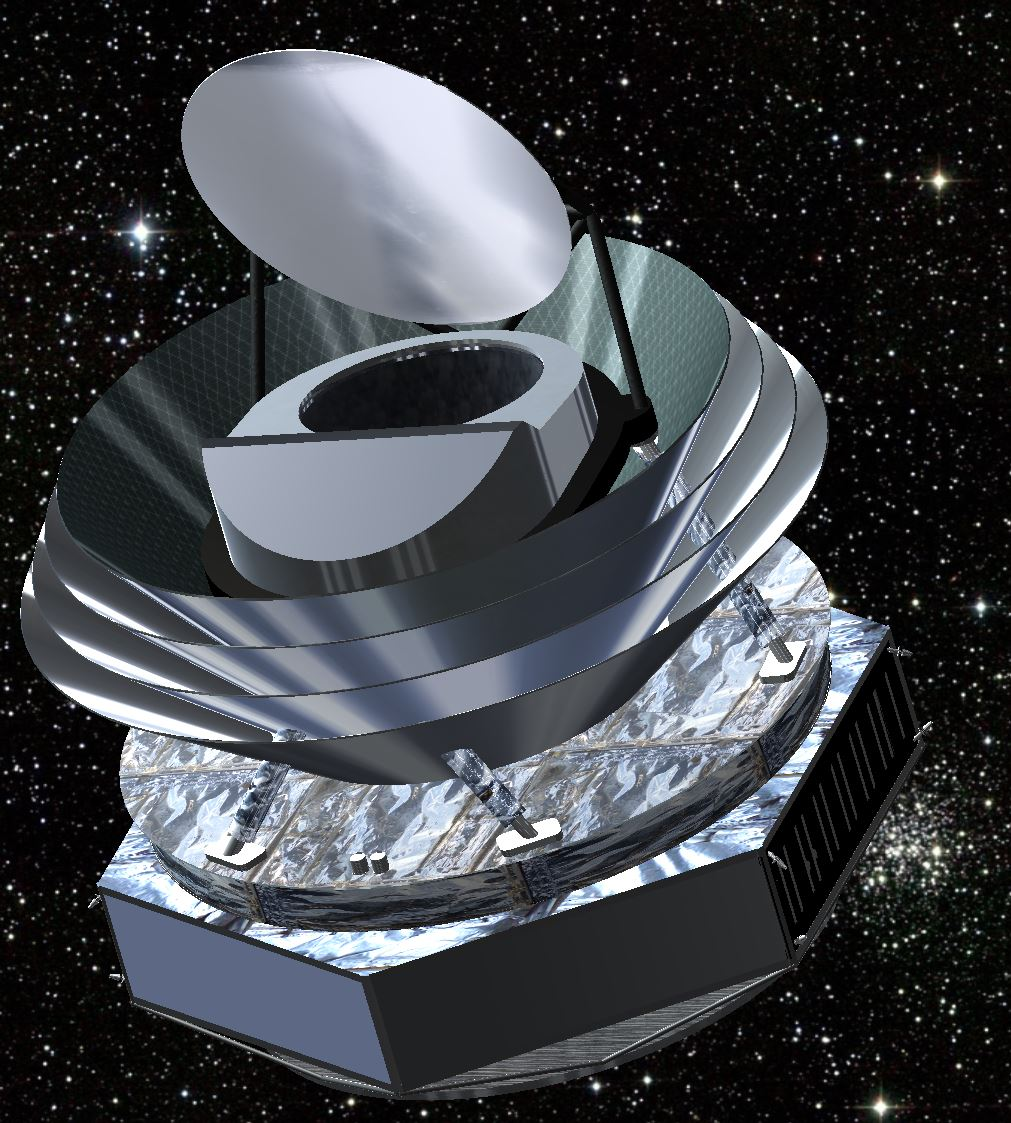
\includegraphics[width=0.31\textwidth]{images/PICO_Image.jpg}
\vspace{-0.25in}
\caption{\captiontext The PICO spacecraft 
\label{fig:pico_rendered} }
\end{wrapfigure}

Building upon a long legacy of successful measurements, the next decade holds tremendous potential for new, exciting \ac{CMB} discoveries.  Such discoveries, delivered by the Probe of Inflation and Cosmic Origins (PICO, Fig.~\ref{fig:pico_rendered}), promise to be revolutionary, affecting physics, astrophysics, and cosmology. PICO is an imaging polarimeter that will scan the sky for 5 years in 21 frequency bands spread between 21 and 799~GHz; see Tables~\ref{tab:specs} and \ref{tab:spec_bands}. It will produce ten independent full-sky surveys of intensity and polarization with a final combined-map noise level equivalent to 3300 \planck\ missions for the baseline required specifications, though in our current best-estimate it would perform as 6400 \planck\ missions.  
%It will produce the first ever full-sky polarization maps at frequencies above 350 GHz, and it will have diffraction limited resolution of 1' at 800~GHz. 

With these capabilities, unmatched by any other existing or proposed platform, PICO will have compelling and broad science deliverables. The mission will address the seven science objectives (SOs), which are listed in Table~\ref{tab:STM}. Delivering this set was the basis for selecting PICO's design and for setting instrument requirements. But PICO's science reach is broader than the baseline set. 

PICO could determine the energy scale of inflation and give a first, direct probe of quantum gravity (SO1, \S~\ref{sec:fundamentalsci}). The mission will attempt to detect the signal that arises from gravitational waves sourced by inflation and parameterized by the tensor-to-scalar ratio, $r$, at a level of $r =5\times10^{-4} \, (5\sigma)$. This level is 100 times lower than current upper limits, and more than 10 times lower than limits forecast by funded experiments.  If the signal is not detected, PICO will constrain broad classes of inflationary models and exclude at $10\sigma$ models for which the characteristic scale in the potential is the Planck scale (SO1 and SO2). The combination of data from PICO and LSST can constrain features in the inflationary potential, the field content during inflation and could rule out all models of slow-roll single-field inflation, marking a watershed in studies of inflation. \comor{reword?}

The mission will have a deep impact on particle physics by measuring the expected sum of the neutrino masses with $4\sigma$ confidence, rising to $7\sigma$ if the sum is near 0.1~eV (SO3). Reaching the $4\sigma$ level can only be done with an instrument that can measure the polarization of the CMB on the largest angular scales, a measurement best done from space, which gives access to the full sky, and with a broad band of frequencies to remove foreground contaminants.  
Cluster counts provided by PICO in combination with followup redshift measurements, and PICO's map of the projected gravitational potentials along the line of site in combination with the LSST gold sample of galaxies, will give two additional independent and equally competitive constraints on the sum of neutrino masses. 

The measurements will either detect or strongly constrain deviations from the standard model of particle physics by counting the number of light particle species $N_{\rm eff}$ in the early universe.  The constraint of $\Delta N_{\rm eff} < 0.06 \, (2\sigma)$ will move the allowed decoupling temperature of a hypothetical new vector particle to temperatures that are 400 times higher than currently determined by \planck\ (SO4). 
%The data will constrain dark matter candidates by pushing down \planck\ constraints on the dark matter annihilation cross section by a factor of 25, specifically at low energy scales, which are not accessible to direct detection experiments. The data will probe the existence of cosmic fields that could give rise to cosmic birefringence. \comor{what about dark energy?}
The data will enable a search for primordial magnetic fields with sufficient sensitivity to rule them out as the sole source for the largest observed galactic magnetic fields; will improve by $\sim$300 constraints on polarization rotation arising from early universe fields that lead to cosmic birefringence, and will thus constrain string theory-motivated axions; and will constrain generic models of dark matter candidates. 

PICO will elucidate the processes affecting the evolution of cosmic structures. It will measure the optical depth to reionization $\tau$ with an error $\sigma(\tau) = 0.002$ limited only by the small number of spatial modes available in the largest angular scale CMB polarization (SO5). The measurement will be used to constrain models of the formation of the first luminous sources, and is a key input to all astrophysical attempts to improve the determination of the sum of neutrino masses. The data will give a map of the projected gravitational potential due to all structures with a \ac{SNR} 14 times higher than \planck , and a catalog of 150,000 clusters extending to their earliest formation redshift. Each of these datasets will be used in combination with other data -- from LSST and from future optical and infrared surveys -- to independently constrain the evolution of the amplitude of linear fluctuations $\sigma_{8}(z)$, with sub-percent accuracy.  

Cross-correlating PICO's map of the thermal Sunyaev--Zeldovich effect with LSST's gold sample of galaxies, a correlation that is forecast to have an \ac{SNR} exceeding 1000, will give precise tracing of the evolution of thermal pressure with $z$. This will be used to place constraints on models of energetic feedback, which is the most uncertain ingredient in models of galaxy formation. 

%Galactic emissions which act as foregrounds and are stronger than the CMB polarized intensity will be separated using PICOs 21 bands spread over a broad frequency bandwidth. 

PICO's maps of the Milky Way will be used to resolve long-standing questions about our own Galaxy. Galactic interstellar dust grains are a link between atoms and molecules and planetary objects, yet their composition and their role in Galactic chemistry is still under debate. Galactic magnetic fields are known to play a key role in the dynamics of gas in the Galaxy, and in determining the efficiency of star formation, but their quantitative contribution relative to turbulence is yet to be determined. With the mission's Galactic dust polarization maps we will constrain dust properties, including composition, temperature, and emissivities (SO6), and we will make maps of the Galactic magnetic field. These detailed 1\arcmin\ resolution maps will be used to quantify the relative roles of turbulence and magnetic fields in the dynamics of the Galaxy and in the observed low star-formation efficiency (SO7). 

PICO will give full-sky maps of intensity and polarization at 21 frequency bands, each much than \planck 's nine frequency maps in intensity and seven in polarization; five PICO bands will have polarization information at frequencies between 385 and 800~GHz that \planck\ did not have. At 385~GHz PICO's noise is 100 times lower than \planck 's at 353~GHz. And PICO's highest resolution is five times finer than \planck 's. Only PICO will provide such full-sky legacy maps. With the six maps at frequencies not accessible to ground-based experiments we will: constrain the early phases of galaxy evolution by discovering 4500 strongly lensed dusty galaxies with $z$ up to 5; investigate the early phases of cluster evolution by discovering 50,000 proto-clusters out to $z\sim4.5$; perform a census of cold dust in 30,000 low $z$ galaxies; make cosmic infrared background maps of the anisotropies due to dusty star-forming galaxies; map magnetic fields in 70 nearby galaxies; and, with 3,000-fold increase relative to \planck\ in the number of independent measurements of magnetic field in our own Galaxy, study how magnetic fields are generated through a combination of turbulence and large-scale gas motion. 

With its broad frequency coverage PICO is better equipped than any other current or planned instrument to separate the detected signals to their original sources of emission.  This capability is most important for the faintest of signals, the telltale of inflation, which is already known to be dominated by Galactic foregrounds. Our simulations indicate that PICO's combination of low noise and multitude of bands is sufficient to separate the inflationary signal from the foregrounds at the required level. But current uncertainties on the parameters characterizing Galactic foregrounds are large and we recommend support for (1) modeling, simulation, and algorithm development for effective foreground separation, and (2) improved Galactic emission measurements with sub-orbital experiments. 
\comor{combine recommendations}?

% [TJP] ------------------------
% [TJP] The Science Traceability Matrix goes here. The table is in stm.tex, but the following LaTeX invocation makes it appear on a double-wide page
\afterpage{%
  % switch to LayoutPageB (includes switching page size)
  \switchToLayoutPageB{}
    \input stm.tex
   \clearpage
% start with LayoutPageA (includes switching page size)
\switchToLayoutPageA{}
% \input stm2.tex  stm2 moved to Legacy science section. (Karl)
% \clearpage
}
% [TJP] end --------------------

Similar to its successful predecessors, WMAP and \planck , PICO will conduct observations from L2, a location that ensures a stable thermal environment.  It will execute ten redundant,  full-sky surveys, each complete within 6 months. The sky scan pattern, which is optimized for control of polarimetric systematic uncertainties, ensures that the measured $I,\, Q$, and $U$ Stokes parameters can be reconstructed by each of the 12,996 polarization-sensitive detectors. The large multiplicity of independent maps and sky surveys, and the stable environment will together give control of systematic uncertainties unmatched by any other platform.

The mission has a single instrument that surveys the sky with the same repeated pattern.  The telescope is a 1.4~m entrance-aperture, two-reflector system, with ambient temperature primary, and 4.5~K actively cooled aperture-stop and secondary. The 0.1~K cooled focal plane is based on three-color pixels coupling the incident radiation to transition-edge-sensor bolometers that are read out using a time-domain multiplexed system. All of these technologies are either already in use by sub-orbital experiments, or are simple extensions to higher or lower frequency bands. We recommend continued support for technology development and maturation in the laboratory and by sub-orbital experiments. 

The science PICO will deliver addresses NASA science objectives, is compelling, timely, and will enrich broad areas of astrophysics. There is a long heritage of space and sub-orbital measurements in these frequency bands; the PICO implementation is a conservative extension of past successes. The mission relies on today's technologies; no new fundamental developments are required. PICO is the only single-platform instrument with the combination of sensitivity, angular resolution, frequency bands, and control of systematic effects that can deliver the compelling, timely, and broad science. We recommend a start for the mission in the next decade. We also recommend support for continued technology development and sub-orbital experiments, and for studying the effects of foregrounds of systematic effects through analytic work and simulations. 


%This scientifically ground-breaking mission is based on technologies that are being used actively today by ground- and balloon-based experiments, but over a more restricted range of frequency band. These technologies will continue to mature by a host of recently funded sub-orbital activities well before the mission's Phase-A. Section~\ref{sec:??}


%All the implementation aspects are mature, benefiting from thousands of person-years of experience studying the sky at these wavelengths. These span over more than 50 years of mapping the CMB and include three enormously successful space missions. This combined experience unambiguously shows that the unlimited frequency coverage and thermally benign environment aboard a space-based platform give unparalleled capability to separate the combination of galactic and cosmological signals and to control systematic uncertainties. These qualities, which are critical ingredients for any next-decade experiment, make PICO the optimal platform for a next generation CMB experiment.

%% End of Martin


%\comor{broad science, unique mission, nothing better in the foreseable future, complementing and enriching other science in the next decade, comparatively cheap, within cost, using existing technologies, relying on extensive community experience both on the ground and in space}

% PICO's data will enrich and complement other astrophysical surveys in the next decade.

%We note that if there {\it is} a detection of the \ac{IGW} signal with $r=0.001$, PICO will make it with high significance in multiple independent patches of the sky. 


%A detection would strongly benefit from confirmation at {\it both} angular scales -- a goal that is beyond the capabilities of ground-based instruments -- {\it and}, for the $\ell = 80$ peak, in several independent patches of the sky -- a goal that is currently not planned for any next decade instrument. 

\end{document}

%see Fig.~\ref{fig:im_1}

%\begin{figure}[!htb]
%\centering
%
\includegraphics[width=4cm]{images/example}
%\caption{example}
%\label{fig:im_1}
%\end{figure}


\section{PICO in Brief (2 pages)}
\documentclass[../PICOReport.tex]{subfiles}

\begin{document}
blah

\begin{figure}[!htb]
\centering

\includegraphics[width=4cm]{../images/example}
 
\label{fig:im_example}
\caption{example}
\end{figure}


\end{document}

\section{Science (22 pgs)}

\subsection{Fundamental Physics}
\documentclass[PICOReport.tex]{subfiles}

\begin{document}

{\bf Gravitational waves and Inflation } \\ %[0.3cm] 
\noindent$\bullet$ {\bf Targets} \hspace{0.1in} Measurements of the \ac{CMB} together with Einstein's theory of general relativity imply that the observed density perturbations must have been created long before the \ac{CMB} was released, and rather remarkably even before the Universe became filled with a hot and dense plasma of fundamental particles. Understanding the mechanism generating these perturbations, which evolved to fill the Universe with structures, is one of the most important open questions in cosmology. In addition to density perturbations, this mechanism may have also produced gravitational waves that would have left a $B$-mode polarization signature in the CMB~\cite{Seljak:1996gy,Kamionkowski:1996zd}. 
%Unlike density perturbations, gravitational waves not only generate primordial temperature and $E$-mode polarization, but also primordial $B$-mode polarization~\cite{Seljak:1996gy,Kamionkowski:1996zd}. 
Any detection of primordial $B$-mode polarization by PICO will constitute evidence for gravitational waves from the same primordial period that created the density perturbations and will open a new window onto this early epoch. Because the dynamics of gravitational waves is essentially unaffected by the plasma, they would be a pristine relic from the earliest moments of our Universe, and their properties would shed light on the mechanism that created the primordial perturbations. 

%\comor{is this a different topic?: PICO's precision measurements of temperature and $E$-mode polarization anisotropy will provide additional detailed information about the statistical properties of the primordial density perturbations generated during this epoch. }\comor{this is a comment on large $\ell$ modes?}

%Measurements of the \ac{CMB} together with Einstein's theory of general relativity imply that the observed density perturbations must have been created long before the \ac{CMB} was released, and rather remarkably even before the Universe became filled with a hot and dense plasma of fundamental particles. Understanding the mechanism generating these perturbations, which evolved to fill the Universe with structures, is one of the most important open questions in cosmology.

%While the dynamics of the plasma produces some amount of gravitational waves, the amplitude 
%is predicted to be too small to be detected in existing or planned experiments. 
%PICO's precision measurements of temperature and $E$-mode polarization anisotropy will provide additional detailed information about the statistical properties of the primordial density perturbations generated during this epoch. 

%The mechanism responsible for the generation of density fluctuations may also produce gravitational waves. PICO will be exquisitely sensitive to the faint imprint that gravitational waves present during recombination leave on the polarization of the CMB. Unlike density perturbations, they not only generate primordial temperature and $E$-mode polarization, but also primordial $B$-mode polarization~\cite{Seljak:1996gy,Kamionkowski:1996zd}. Any detection of primordial $B$-mode polarization by PICO would constitute evidence for gravitational waves from the same primordial period that created the density perturbations and open a new window onto this early epoch.

Inflation, a period of nearly exponential expansion of the early Universe~\cite{Guth:1980zm,Linde:1981mu,Albrecht:1982wi,Starobinsky:1980te}, is the leading paradigm explaining the origin of the primordial density perturbations~\cite{Mukhanov:1981xt,Guth:1982ec,Hawking:1982cz,Starobinsky:1982ee,Bardeen:1983qw}. It predicts a nearly scale invariant spectrum of primordial gravitational waves originating from quantum fluctuations~\cite{Starobinsky:1979ty}. 
%\sout{In this sense, a detection of primordial $B$-modes would be the first observation of a phenomenon associated with quantum gravity~\cite{Krauss:2013pha}.} \comor{moved} 
Measurements of the \ac{CMB} are the only foreseeable way to detect these gravitational waves.

%\sout{Because the spectrum is scale-invariant, one may hope to detect primordial gravitational waves over a wide range of frequencies, including, for example, at LIGO or LISA frequencies. However, as a consequence of the expansion of the Universe, the energy density in the gravitational waves rapidly dilutes with increasing frequency, and observations of the CMB provide the easiest, and (for the foreseeable future) only way to detect gravitational waves at this scale. }

\begin{figure}[!thb]
\centering
\hspace{-0.15in}
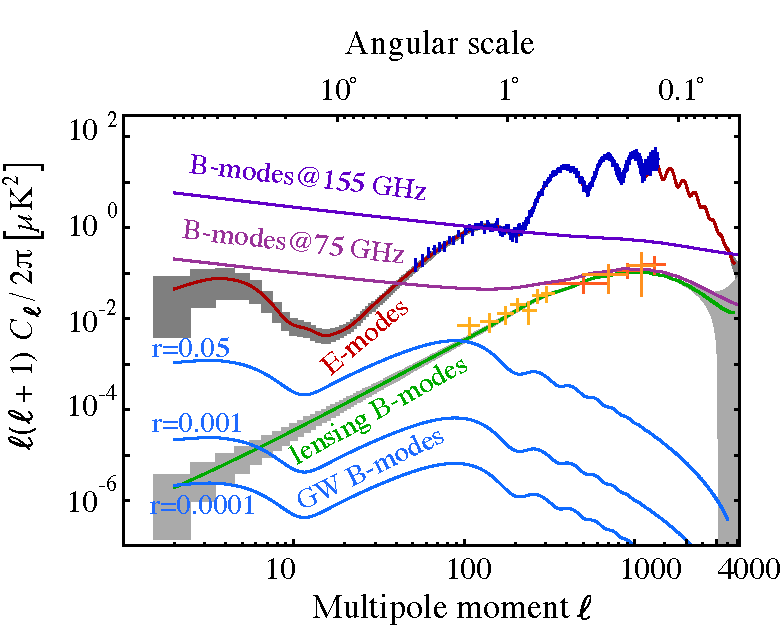
\includegraphics[width=3in]{images/cmb_powspec_PICOv4p1_v2.pdf}
\hspace{-0.15in}
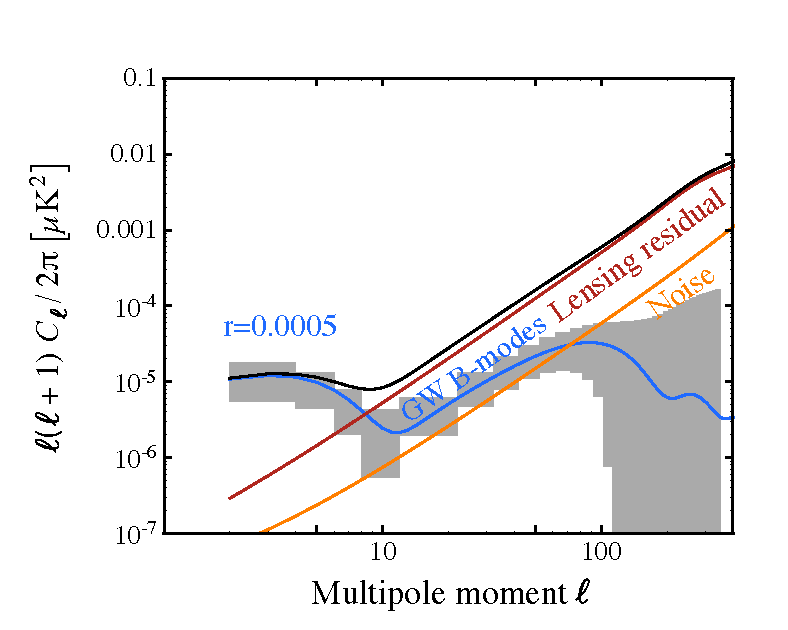
\includegraphics[width=2.9in,trim= 0cm 0.2cm 0cm 0cm]{images/cmbbb_powspec_PICOv4p1.pdf}
\caption{\captiontext With PICO's \comred{baseline} configuration we will measure the $EE$ (left, red) and lensing $BB$ (green) angular power spectra with high precision (grey). PICO's goal is to detect $r= 5\times 10^{-4}\, (5\sigma)$ (right, grey). This forecast includes PICO's \comred{80\%} delensing (red) and foreground separation. The \comred{baseline} noise level (right, orange) allows detection of even lower levels; we expect foreground separation to limit performance.  As an example we show the $BB$ spectra of Galactic emission on the cleanest $60\%$ of the sky at 75 and 155~GHz (left, purple). They largely dominate the cosmological signals. Also shown are measurements of lensing from current experiments (left, orange)~\citep{PB_BB, keisler2015, actpol_lensing_BB, Array:2015xqh}, \planck 's $EE$ measurements (left, dark blue)~\citep{Planck2018_I}, and the $BB$ spectrum produced by \ac{IGW} with different values of $r$ (cyan). }
\label{fig:clbb}
\end{figure}

The strength of the signal, quantified by the tensor-to-scalar ratio $r$, is a direct measure of the expansion rate of the Universe during inflation. Together with the Friedmann equation, it reveals one of the most important characteristics of inflation: its energy scale.\footnote{In some models of inflation the one-to-one correspondence between $r$ and the energy scale of inflation does not hold because there are additional sources of gravitational waves~\cite{Namba:2015gja}. However, in these models the signal is highly non-Gaussian and could be distinguished from quantum fluctuations.}  A detection of $r$  "would be a watershed discovery", a quote from the 2010 decadal panel report~\citep{blandford2010}. The combination of data from \planck\ and the BICEP/Keck Array give the strongest constraint to date, $r<0.06\,\, (95\%)$~\citep{2018arXiv181005216A}. Next decade S3 efforts strive to reach $\sigma(r)=2 \times10^{-3}$~\citep{SOscience, biceparray}.

PICO's goal is to detect primordial gravitational waves if inflation occurred at an energy scale of at least $5\times 10^{15}\,\rm{GeV}$, or equivalently $r= 5\times 10^{-4} \, (5\sigma)$ (SO1 in Table~\ref{tab:STM} and Figure~\ref{fig:clbb}). 
A detection will have profound implications for fundamental physics because it will provide evidence for a new energy scale tantalizingly close to the energy scale associated with grand unified theories, probe physics at energies far beyond the reach of terrestrial colliders, and be the first observation of a phenomenon associated with quantum gravity~\cite{Krauss:2013pha}.

There are only two classes of slow-roll inflation in agreement with current data that naturally explain the observed value of the spectral index of primordial fluctuations $n_{\rm s}$~\cite{Aghanim:2018eyx}. The first class is characterized by potentials of the form $V(\phi)\propto\phi^p$. This class includes many of the simplest models of inflation, some of which have already been strongly disfavored by existing observations. Select models in this class are shown as blue lines in Fig.~\ref{fig:nsr}. If the constraints on $n_{\rm s}$ tighten by about a factor of two with the central value unchanged, and the upper limit on $r$ improves by an order of magnitude, this class would be ruled out. 

The second class is characterized by potentials that approach a constant as a function of field value, either like a power law or exponentially. Two representative examples in this class are shown as the green and gray bands in Fig.~\ref{fig:nsr}. This class also includes $R^2$ inflation, which predicts a tensor-to-scalar ratio of $r\sim 0.004$. All models in this class with a characteristic scale in the potential that is larger than the Planck scale predict a tensor-to-scalar ratio of $r\gtrsim 0.001$. 
%\sout{Different values of characteristic scales are indicated by the darker lines in Fig.~\ref{fig:nsr}. } \comor{moved to Figure.}

Many microphysical models in this class possess a characteristic scale that is super-Planckian. PICO will either detect gravitational waves with high confidence or will exclude all models with a Planckian characteristic scale with high significance. But not all models have a super-Planckian characteristic scale. The Goncharov-Linde model is an example with a somewhat smaller characteristic scale. It predicts a tensor-to-scalar ratio of $r\sim 4\times 10^{-4}$~\cite{Goncharov:1983mw}, still within reach of PICO. In addition, there are models with significantly smaller values that are out of reach, but distinguishing between models with sub- and super-Planckian characteristic scales would provide much needed guidance to discriminate between classes of ideas for the earliest moments of our universe.


\begin{figure}[!thb]
\parbox{4.5in}{\centerline{
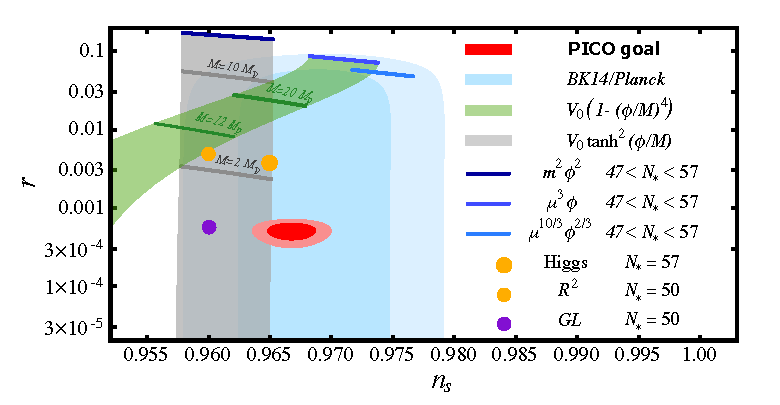
\includegraphics[width=4.5in]{images/nsrlabeledrp0005_PICOv4p1.pdf}}}
\parbox{1.8in}{
\caption{\captiontext  Current $1\sigma$ and 2$\sigma$ limits on $r$ and $n_{\rm s}$ (cyan) and forecasted constraints for a fiducial model with $r = 0.0005$ for PICO together with predictions for selected models of inflation. Characteristic super-Planckian scales in the potentials are marked with darker lines. }
\label{fig:nsr}}
\end{figure}

\noindent$\bullet$ {\bf Observational Considerations} \hspace{0.1in} The $BB$ angular power spectrum measured by PICO will have contributions by Galactic sources of emission and `lensing' $B$-modes, created by gravitational lensing of $E$-modes as the CMB photons traverse the gravitational potentials throughout the Universe (Fig.~\ref{fig:clbb}). In case of an $r$ detection, there will be two additional features due to the inflationary signal. One is the `recombination peak' at $\ell \sim 80$ and the other is the `reionization peak' at multipoles of $\ell\lesssim 10$. 

The Galactic signals act as foregrounds and uncertainty in the characterization of these foregrounds already now limits our ability to constrain $r$. PICO's goal for reaching $\sigma(r) = 1\times10^{-4}$ is driven by estimates of the efficacy of foreground separation, not noise.  An analytic performance forecast accounting for PICO's statistical noise level and a foreground model that has polarized emission from two components of dust, synchrotron radiation, and correlations between synchrotron and dust emission, gives $\sigma(r) = 2\times10^{-5}$, five times lower than our baseline goal. Our goal is set based on end-to-end, map-based simulations, which include physical effects known to exist but not captured in the analytic forecasts; see Section~\ref{sec:signal_separation}.   
%such as spatial variation of dust temperatures, dust-to-gas ratio, dust composition, which lead to spatial variation of the spectral dependence, are expected to weaken the constraints. In Section~\ref{sec:foregrounds} we discussed PICO's capability to separate foregrounds in more detail. 

When the tensor-to-scalar ratio $r \simeq 0.01$, the $BB$ lensing and inflation spectra are comparable in magnitude at the recombination peak $(\ell \sim 80)$. For lower levels of $r$, the lensing $B$-mode dominates, but the $B$-mode maps can be `delensed' if the polarization maps are measured with few-arcmin resolution and sufficient depth~\citep{2004PhRvD..69d3005S,2012JCAP...06..014S}. Forecasts for PICO show that at least 73\% of the lensing $B$-mode power can be removed for the baseline configuration, after accounting for Galactic foreground separation. As much as 84\% will be removed for the CBE and for milder foreground contamination. For measuring the recombination peak, delensing is essential to reach PICO's limits on $r$, and this was a driver in choosing the resolution of the instrument. 
% PICO will be relying on its own data to conduct delensing, thus avoiding increased noise from the need to cross-calibrate experiments, identify common observing areas on the sky, not having frequency-band coverage at the appropriate resolution to remove foregrounds, or from other systematic uncertainties.

For the levels of $r$ targeted by PICO, the $BB$ reionization signal $(\ell \sim 5)$ has somewhat higher level than the lensing spectrum, but the map-level foregrounds at this angular scale are at least two orders of magnitude brighter.  PICO's instrument temporal stability, absence of atmospheric noise, full-sky coverage, and unmatched capability to characterize and separate foregrounds make it the most suitable instrument to measure these lowest multipoles. No S3 experiments have measured or plan to measure $B$-modes at $\ell<40$ that reach to $\sigma(r) < 0.006$ at the lowest multipoles~\citep{class,piper}. 

If an inflationary $B$-mode signal is detected, it is important to characterize its entire $\ell$ dependence, in both the predicted reionization and  recombination peaks. Furthermore, the strongest constraints on $r$ are obtained when using all available $\ell$ modes. And the PICO full sky coverage will enable detection of the recombination peak in several independent patches of the sky, giving an important systematic cross-check. 

\noindent$\bullet$ {\bf Scalar Spectral Index and Non-Gaussianity} \hspace{0.1in} Models of the early Universe  differ in their predictions for the scalar spectral index $n_{\rm s}$ and its scale dependence $n_{\rm run}$. PICO will improve $n_{\rm s}$ and $n_{\rm run}$ constraints by a factor of three relative to \planck\ and will thus have more discriminating power between different models. 

The simplest models of inflation predict primordial fluctuations that are very nearly Gaussian. But only certain classes of multi-field inflation produce a level of non-Gaussianity large enough to exceed $f_{NL} =1$, where $f_{NL}$ is a parameter quantifying the level of non-Gaussianity (Fig.~\ref{fig:fnlconstraint}).  \comor{PICO will probe the statistical properties of the primordial perturbations over a wide range of scales and will improve constraints on departures from Gaussianity by a factor of two to three depending on the precise form of the departure from non-Gaussianity. By cross-correlating the lensing map with large-scale structure data from LSST it may even be possible to reach a theoretically important threshold (see, e.g.~\cite{2014arXiv1412.4671A} and references therein) and constrain local non-Gaussianity to better than $\sigma(f_{NL})=1$. }

\begin{figure}[h]
\hspace{-0.in}
\parbox{3.1in}{\centerline {
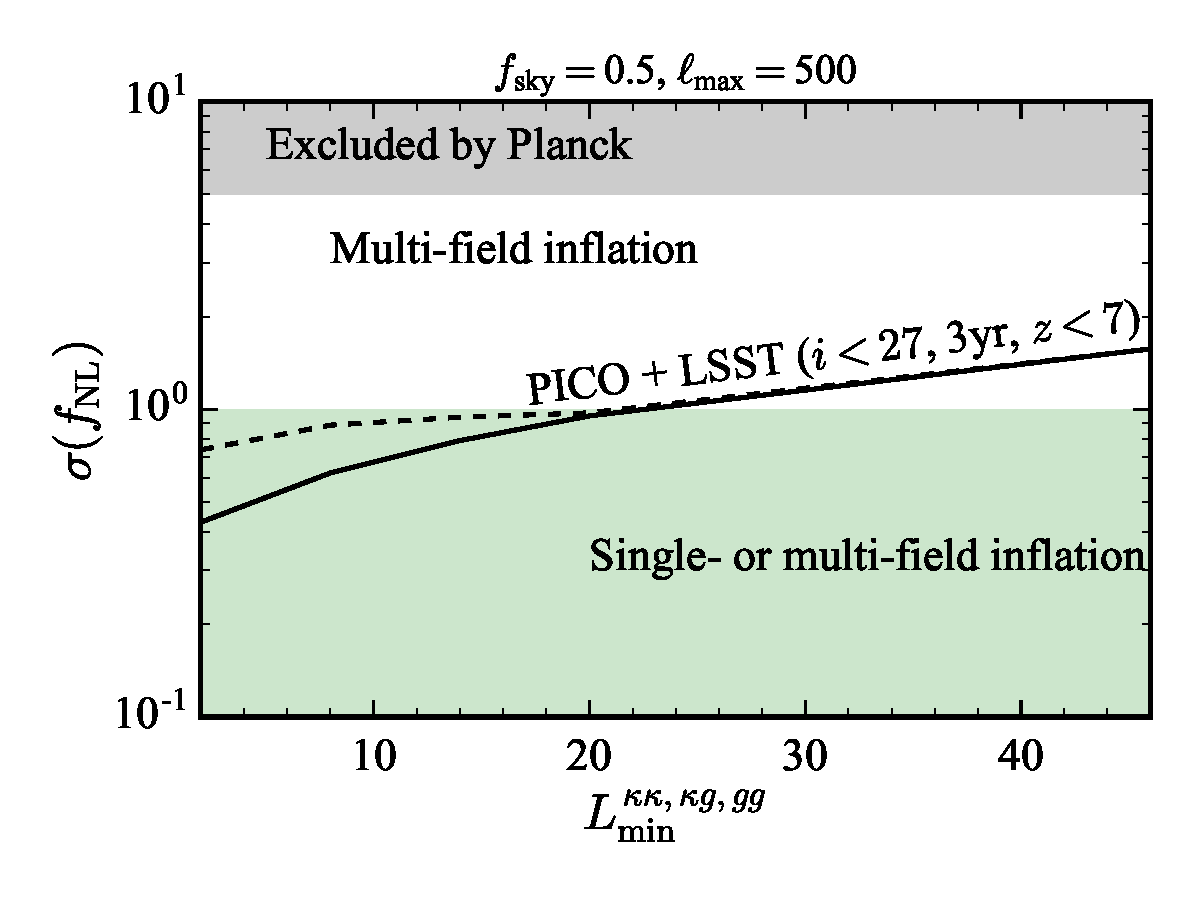
\includegraphics[width=2.95in]{images/PICO_fnl_lmin_PICOv4.1b_deproj0_SENS0.pdf} } }
\hspace{0.in}
\parbox{3.3in}{
\caption{\captiontext
Forecasted sensitivity to the parameter describing primordial non-Gaussianity of the local type for the PICO CMB lensing map together with three years of the LSST survey, as a function of the minimal multipole used in the analysis (f$_{\rm sky} = 50\%$). A value of $\sigma (f_\mathrm{NL}) \simeq 1$ is a well-motivated theoretical target.
\label{fig:fnlconstraint}
} }
\vspace{-0.1in}
\end{figure}

\comor{One can use correlations between large-scale structure tracers with different clustering bias factors and measure the relative difference between their clustering power spectra to effectively cancel cosmic variance~\citep{2009PhRvL.102b1302S,2018PhRvD..97l3540S}; this can constrain physics that affects the biasing of objects on large scales, such as primordial local non-Gaussianity~\citep{2008PhRvD..77l3514D}.  In Fig.~\ref{fig:fnlconstraint} we show the expected constraints for the CMB lensing field as reconstructed with PICO, in cross-correlation with  three years of the LSST survey. It can be seen that depending on the minimal multipole that can be used in the cross correlation, which is uncertain in both LSST and the PICO lensing map, the well-motivated theory target of $\sigma (f_\mathrm{NL}) \simeq 1$ \citep{2014arXiv1412.4671A} can be within reach. Values of $f_\mathrm{NL}$ at or above this level are a generic prediction of multi-field inflationary models.}

\vspace{0.1in}
%%%%%%%%%%%%%%%%%%%%%%%%%
\parindent = 0pt
{\bf Fundamental Particles: Light relics, Dark Matter, and Neutrinos} \\ %[0.3cm]
\parindent = 15pt
%\vspace{0.1in}
%%%%%%%%%%%%%%%%%%%%%%%%%
$\bullet$ {\bf Light Relics} \hspace{0.1in} In the inflationary paradigm, the Universe was reheated to temperatures of 
at least 10 MeV and perhaps as 
high as $10^{12}$ GeV.  At these high temperatures, even very weakly interacting or very massive particles, 
such as those arising in extensions of the Standard Model of particle physics, can be produced in large 
abundances~\cite{1979ARNPS..29..313S,Bolz:2000fu}.  As the Universe expands and cools, 
the particles fall out of equilibrium, leaving observable signatures in the CMB power spectra.
Through these effects the CMB is a sensitive probe of neutrino and of other particles' properties.  

% sensitive probe of the fundamental particle content in the Universe
% large abundance, but not large enough to leave present day signatures? or they decay?
% don't like the words 'extensions of ...' suggests very unlikely things. 

One particularly compelling target is the effective number of light relic particle species $\Neff$. The canonical value with three neutrino families is $\Neff = 3.046$. Additional light particles contribute a change $\Delta \Neff$ that is a function only of the decoupling temperature and the effective degrees of freedom of the particle, $g$. The magnitude of $\Delta\Neff$ is quite restricted, even for widely varying decoupling temperatures $T_{F}$. A range $ 0.027\,g \leq \ \Delta \Neff \leq 0.07\,g$ corresponds to a range in $T_{F}$ spanning decoupling during post-inflation reheating (0.027$g$) down to lower $T_{F}$ with decoupling occurring just prior to the QCD phase transition ($0.07g$).
%Additional light particles contribute a universal change to $\Neff$ that is a function only of the decoupling temperature and the effective degrees of freedom of the particle, $g$. Furthermore, the range of $\Delta\Neff$ is quite restricted, even for widely varying decoupling temperatures $T_{F}$ with the range $ 0.027\,g \leq \ \Delta \Neff \leq 0.07\,g$ corresponding to decoupling at higher temperatures during post-inflation reheating (0.027$g$) to lower temperatures shortly prior to the QCD phase transition ($0.07g$).

Information about $\Neff$ is gleaned from the $TT$ and $EE$ power spectra. For an experiment like PICO, which has sufficient resolution to reach cosmic-variance-limited measurement\footnote{A measurement is cosmic-variance-limited when the measurement uncertainty is dominated by the statistics of observing the finite number of Fourier modes available in our Universe.} of $EE$ up to $\ell =2300$, the two additional most important parameters for improving constraints are the fraction of sky observed $f_{\rm sky}$ and the noise (Fig.~\ref{fig:Neff_future}, left). The PICO baseline will use data from 70\% of the sky to constrain $\Delta \Neff < 0.06 \, (95\%)$. \footnote{The CMB $EE$ and the Galactic foregrounds $EE$ and $BB$ spectra are comparable in level (Fig.~\ref{fig:clbb}). With 21 frequency bands PICO should be able to separate signals at the mild levels necessary for 70\% of the sky.} This constraint, which is a factor of 4.7 improvement relative to \planck~($\Delta \Neff < 0.28$, 95\%) and will not be matched by any currently funded effort, opens up a new range of temperatures in which to detect the signature of light relic species. If no new species are detected, then the lowest temperature $T_{F}$ at which any particle with spin could have fallen out of equilibrium will move up by a factor of 400 (Fig.~\ref{fig:Neff_future}, right). 

\begin{figure}[t!]
\begin{center}
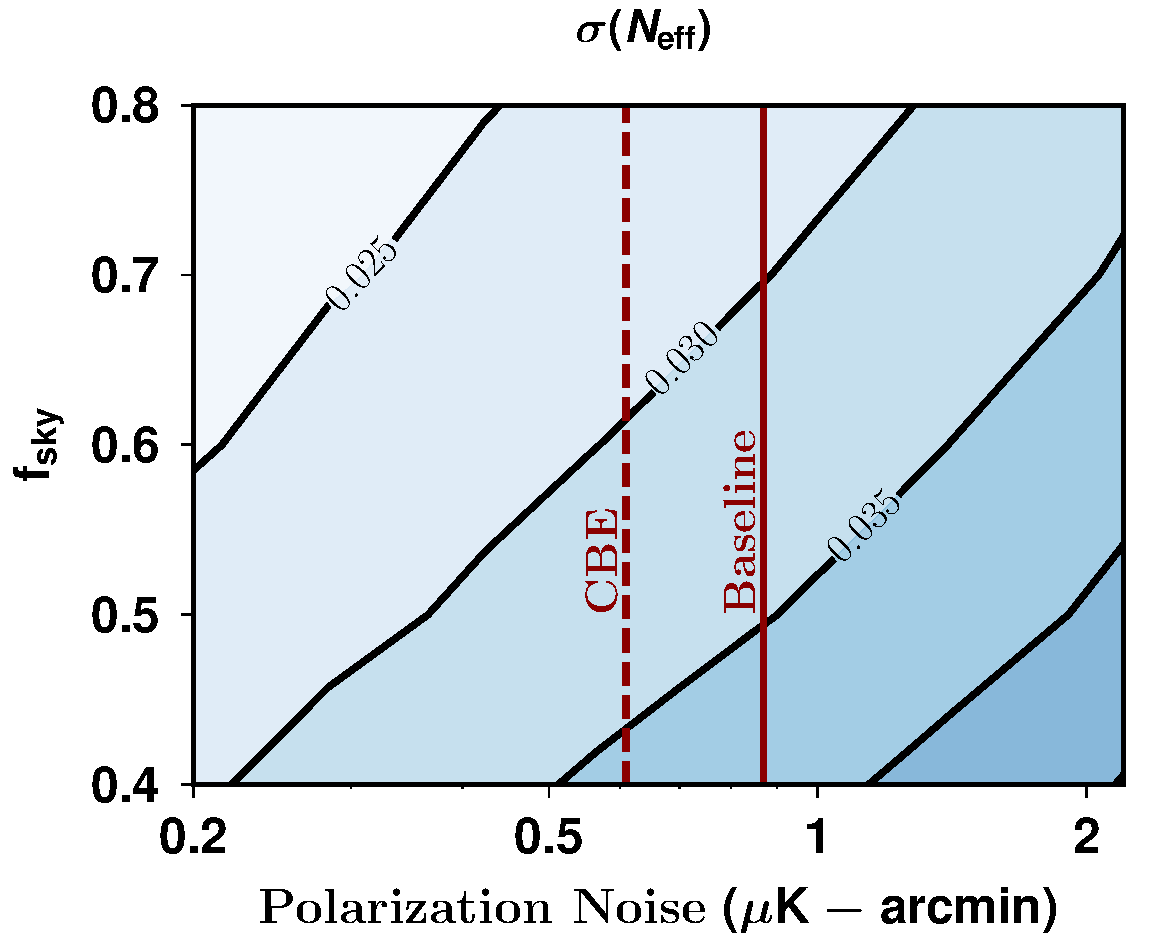
\includegraphics[width=0.45\textwidth]{images/Neff_final.pdf}
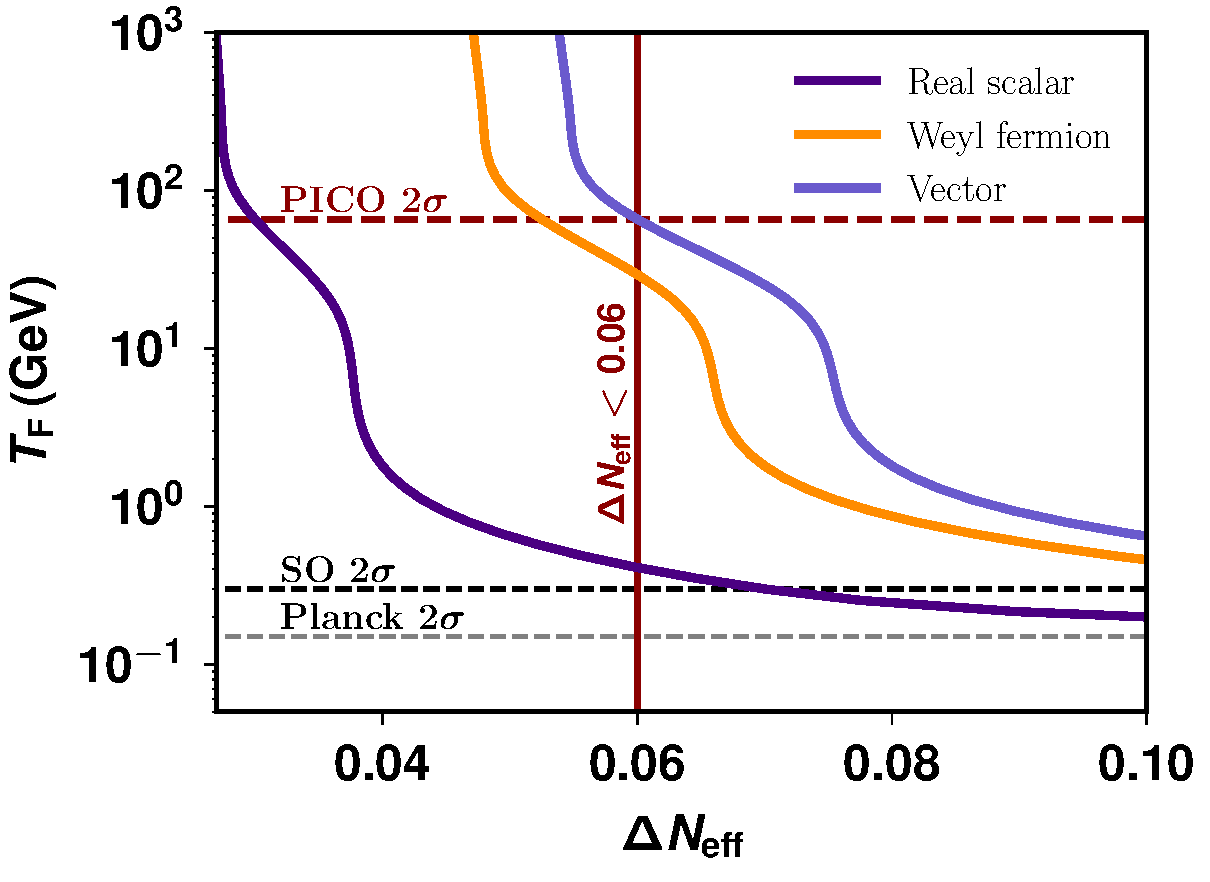
\includegraphics[width=0.47\textwidth]{images/Tf_pico.pdf}
\vspace{-0.15in}
\caption{ \captiontext PICO will achieve a constraint $\Delta \Neff < 0.06\, (95\%)$ (left, $2\sigma$ contours shown) in the baseline configuration (vertical solid) using its cosmic-variance-limited measurement of $EE$ for $\ell \leq 2300$, and 21 frequency bands to utilize data over 70\% of the sky (5\arcmin\ resolution assumed) . This constraint translates to moving up the lowest decoupling temperature $T_{F}$ for vector, Weyl Fermion, and scalar particles by a factor of 400, 200, and 6, respectively, relative to \planck\ (right, dash black, only $T_{F}$ for vector particle is shown). We also show the projected vector particle limit for the Simons Observatory~\citep{SOscience}. }
\label{fig:Neff_future}  
\end{center}
\vspace{-0.15in}
\end{figure}

While our theoretical target for $\Neff$ is defined by particles that decoupled long before neutrinos did, there are a number of well-motivated scenarios in which the thermal evolution of the Standard Model is altered after the time of neutrino decoupling.  These scenarios will change the relationship between $\Neff$ as measured in the CMB relative to the value of $\Neff$ that affects BBN and the production of helium, which is quantified through the helium fraction $Y_p$.  For example, the decay of a thermal relic into photons after nucleosynthesis would reduce $\Neff$ in the CMB but would could leave $Y_p$ unaltered from its Standard Model value.  PICO will make a simultaneous measurement of $\Neff$ and $Y_p$ with $\sigma(\Neff) = 0.08$ and $\sigma(Y_p) =0.005$, respectively, giving a 2\% uncertainty on the value of $Y_p$. These uncertainties are equivalent to those available with other astrophysical measurements, but the systematic uncertainties are entirely different. Systematic uncertainties currently limit our knowledge of $Y_{p}$. 

%%%%%

\noindent$\bullet$ {\bf Dark Matter} \hspace{0.1in} Cosmological measurements have already confirmed the existence of one relic that lies beyond the Standard Model: dark matter. \ac{CMB} experiments are effective in constraining dark matter candidates in the lower mass range, which is not available for terrestrial direct detection experiments~\citep{Madhavacheril:2013cna,Green:2018pmd}. 

Interactions between dark matter and protons in the early Universe create a drag force between the two cosmological fluids, damping acoustic oscillations and suppressing power in density perturbations on small scales. As a result, the CMB temperature, polarization, and lensing power spectra are suppressed at high multipoles relative to a Universe without such drag forces.  This effect has been used to search for evidence of dark matter-proton scattering over a range of masses, couplings, and interaction models~\citep{2002astro.ph..2496C, 2004PhRvD..70h3501S, Dvorkin:2013cea, 2018PhRvL.121h1301G,2018arXiv180108609B, 2018PhRvD..97j3530X, 2018arXiv180800001B, 2018PhRvD..98b3013S}, to test the possibility of an interacting dark-matter sub-component~\citep{2018arXiv180800001B}, and to provide consistency tests of dark matter in the context of the anomalous 21-cm signal reported by the EDGES collaboration~\citep{2018Natur.555...71B,2018Natur.555...67B,2018arXiv180800001B,2018arXiv180711482K}.

%\planck\ data and funded, next generation CMB instruments will place cosmic-variance-limited constraints on conventional WIMP dark matter candidate~\citep{Madhavacheril:2013cna,Green:2018pmd}. \comor{add simons citation}. PICO will constrain lower mass dark matter candidates in a mass range that is not available for terrestrial direct detection experiments. 

%For a conventional WIMP candidate, the CMB places very stringent constraints on its properties through the signature of its annihilation~\cite{Peebles:2000pn, Chen:2003gz, Padmanabhan:2005es}. Most of this information is in the $EE$ power spectrum at $50 < \ell < 300$, which is well-measured by \planck~and will approach the \comor{will approach? or will be?} cosmic-variance limit with existing ground-based surveys~\cite{Madhavacheril:2013cna,Green:2018pmd}.  An entirely complementary way to probe dark matter is to search for evidence of its interactions with other species in cosmological data. Since a lower mass translates to a higher number density of scattering centers, the CMB is particularly useful for probing the low-mass regime and is sensitive to large, nuclear-scale cross sections. 
 
PICO's constraining power comes primarily from making high \ac{SNR} maps of the lensing-induced deflections of polarized photons, which are discussed in Section~\ref{sec:extragalacticsci}.  For a spin-independent velocity-independent contact-interaction, chosen as our fiducial model, PICO will improve upon \planck 's dark matter cross-section constraints by a factor of 25 over a broad range of candidate masses that will not be probed by direct detection experiments (Fig.~\ref{fig:DM_baryons}, right). 
%The constraints are complementary to those forthcoming from direct detection experiments, which are more sensitive at the high mass range.  
%\comor{need to decide what to do with this section.}

%In the right panel of Fig. \ref{fig:DM_baryons}, we present current and projected upper limits on the dark matter-proton interaction cross section as a function of dark matter mass, for a spin-independent velocity-independent contact-interaction (chosen as our fiducial model). Shaded regions are excluded at 95$\%$ confidence by {\planck} \cite{2018PhRvL.121h1301G} and direct-detection measurements \cite{2018PhRvD..97l3013K}. When we compare current limits obtained from {\planck} with projections for PICO sensitivity (dashed line), we note that PICO can deliver a substantial improvement over the current CMB limits, across the entire dark-matter mass range considered.  Most of the constraining power in the case of PICO (and ground-based next-generation measurements with similar white-noise levels) comes from the measurement of the lensing power spectrum $C_\ell^{\phi \phi}$ \cite{2018arXiv180610165L}.
%
\begin{figure}[t]
\begin{center}
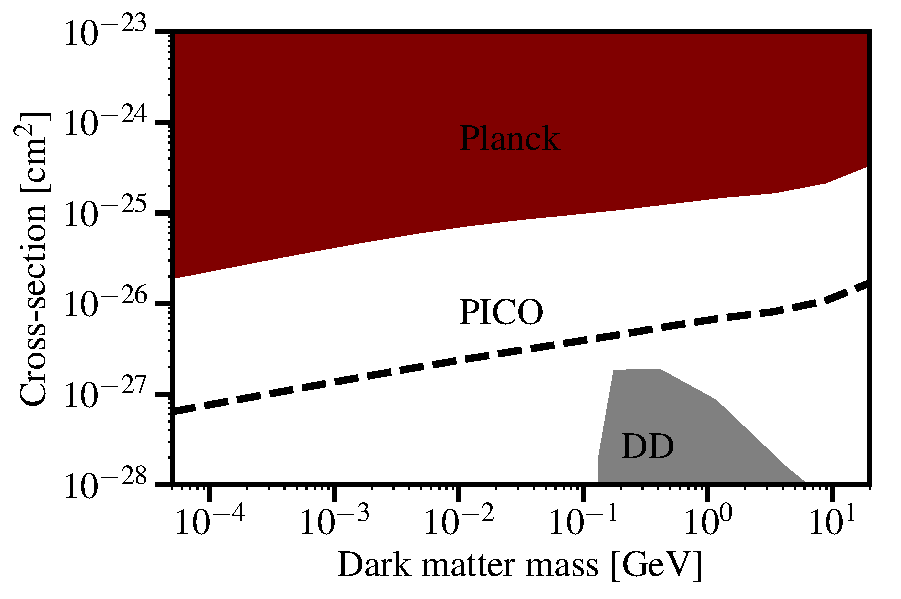
\includegraphics[width=0.50\textwidth]{images/pico_dd3.pdf}
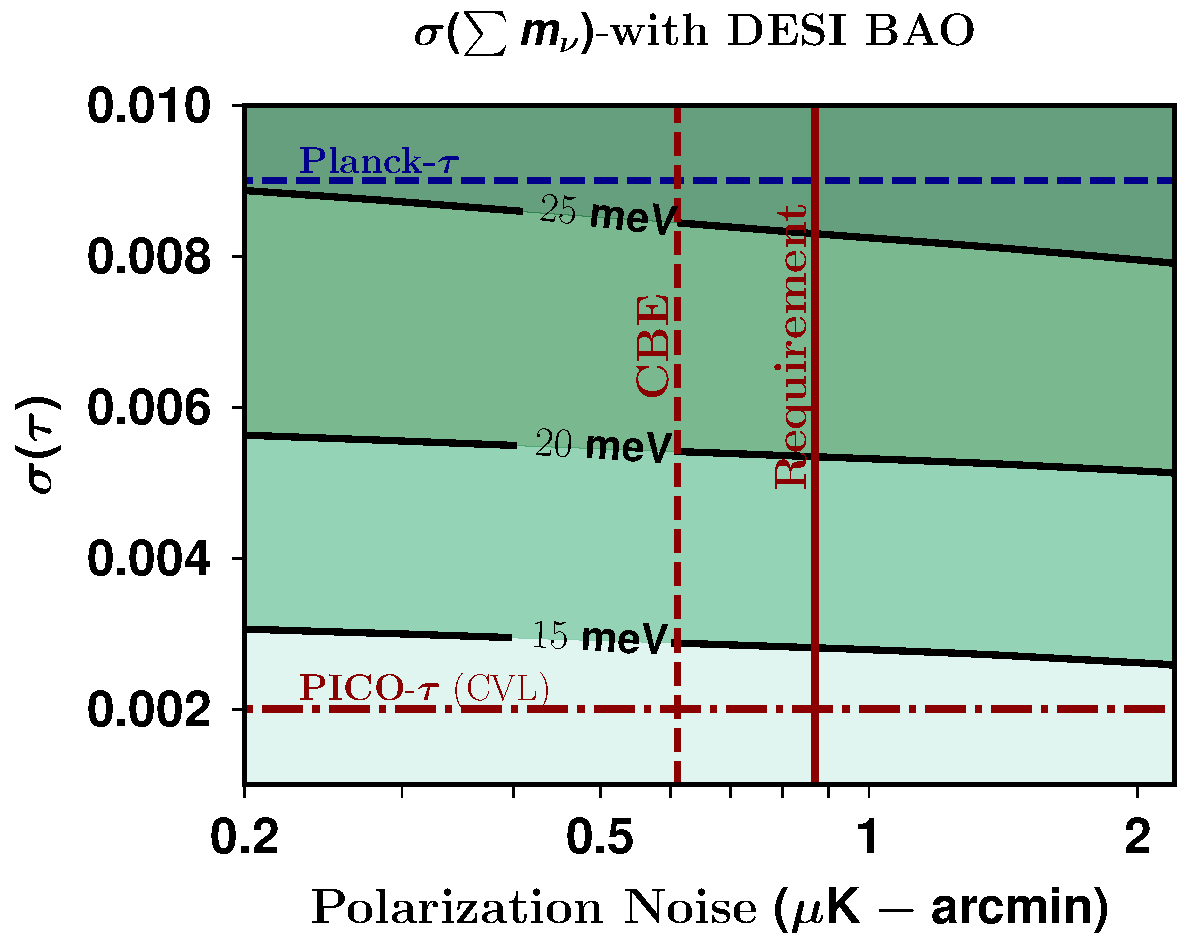
\includegraphics[width=0.48\textwidth]{images/Mnu_tauprior_final.pdf}
\caption{\captiontext {\bf Left:} PICO will give a factor of 25 more stringent constraint on spin-independent velocity-independent dark matter scattering cross-section (dash) relative to current \planck\ 95\% confidence limit (red)~\citep{2018PhRvL.121h1301G}. Terrestrial direct detection experiments are expected to give complementary and stronger constraints, but only for the higher dark matter masses (grey)~\cite{2018PhRvD..97l3013K}. 
{\bf Right:} Using cosmic-variance-limited (CVL) measurement of $\tau,\, \sigma(\tau)=0.002$, \ac{BAO} information from DESI, and 21 frequency bands to separate foregrounds over 70\% of the sky, PICO will reach $\sigma(\Sigma m_{\nu}) = 14$~meV (contours) giving at least $4\sigma$ detection of the minimal expected sum of neutrino masses $\Sigma m_{\nu} = 58$~meV. 
\label{fig:DM_baryons} }
\end{center}
\vspace{-0.15in}
\end{figure}
%

Axion is another dark matter candidate that is well motivated by string theory~\citep{Arvanitaki_etal}, and that is consistent with straightforward extensions of the standard model of particle physics~\citep{peccei,weinberg,wilczek}. For an axion mass in the intermediate range $10^{-30} < m_a< 10^{-26} $~eV, current measurements constrain its fraction to be equal to or less than 2\% of the total dark matter density. If 2\% of the total dark content is made of axions, PICO's measurement of the $TT$, $TE$ and $EE$ spectra with additional constraints from the lensing reconstruction will give a $6\sigma$ detection, a factor of 10 improvement relative to \planck , 
%and 1.5 relative to Planck and SO, respectively,  
profoundly shaping our understanding of the nature of dark matter and its small-scale clustering. "

\noindent$\bullet$ {\bf Neutrino Mass} \hspace{0.1in} \label{neutrino_fundamental} The origin and structure of the neutrino masses is one of the great outstanding  questions about the nature of the Standard Model particles.  
%Measurements of neutrinos in the lab have revealed much  about the mass differences and mixing angles.  
Cosmology offers a  measurement of the sum of the neutrino masses $\sum m_\nu$ through the gravitational influence of the non-relativistic  cosmic neutrinos.  The current measurement of $\Neff = 2.99 \pm 0.17$~\citep{Planck2018_VI} already confirms the existence of these neutrinos at $>10\sigma$ and their mass implies that they will contribute to the matter density at low redshifts.  The best current mass constraint arises from a combination of  \planck~and BOSS \ac{BAO} giving $\sum m_\nu < 0.12$ eV (95\%) \cite{Planck2018_VI}.
\comor{should we say 'and their minimal mass implies that they will contribute at least 3\%(?) of the total matter density at low..}

Cosmological measurements are primarily sensitive to the suppression of power on small scales after the neutrinos become non-relativistic, which can be measured via CMB lensing, or weak lensing in galaxy surveys.  However, these measurements are limited by our knowledge of the amplitude of the primordial fluctuation power spectrum $A_s$ because they only constrain the combination $A_s e^{-2 \tau}$. Although many surveys hope to detect $\sum m_\nu$, any detection of the minimum value expected from particle physics, $\sum m_\nu = 58$~meV, at more than $2 \sigma$ will require a better measurement of $\tau$.
% and thus do not provide a high-precision measurement of either $A_s$ or $\tau$ separately.  \comor{we mention 'galaxy survey', but don't complete the thread of thought. Do we mean to say that the galaxy survey will be limited by the same degeneracy?}

The best constraints on $\tau$ come from the $EE$ spectrum at $\ell < 10$, which require measurements over the largest angular scales, and good separation of Galactic foreground sources of emission. The current limit of $\sigma({\tau}) = 0.007$ is from \planck~\cite{planck2016_xlvi}. \comor{I notice we are quoting Planck2016; are there newer constraints} 
%Forecasts for a CMB measurement of $\sum m_\nu$ using the lensing $B$-modes~\cite{Kaplinghat:2003bh} are shown in Fig.~\ref{fig:DM_baryons}.  
With the current uncertainty in $\tau$ one is limited to  $\sigma(\sum m_\nu) \gtrsim 25$ meV, after including forthcoming \ac{BAO} information (Fig.~\ref{fig:DM_baryons}, right); no other survey or cosmological probe will improve this constraint, unless a more accurate measurement of $\tau$ is made. One of the S3 experiments is attempting to measure the lowest $\ell$'s~\citep{class}. A space mission with its access to the entire sky and broad frequency coverage is the most suitable platform for the measurement. PICO will reach the cosmic-variance limit uncertainty on $\tau$, $\sigma(\tau) \sim 0.002$, and will therefore reach $\sigma(\sum m_\nu) = 14$ meV when combined with measurements of \ac{BAO} from DESI or Euclid~\cite{Levi:2013gra} (PICO alone would reach $\sigma(\sum m_\nu) = 43$ meV).  This measurement will give a $4\sigma$ detection of the minimum sum. 

%Robustly detecting neutrino mass at  $> 3\sigma$ in any cosmological setting is only possible with an improved measurement of $\tau$, like the one achievable with PICO. This measurement will give $\sum m_\nu>0$ at greater than $4\sigma$ or would exclude the inverted hierarchy ($\sum m_\nu > 100$ meV) at 95\% confidence, depending on the central value of the measurement.  Lab-based measurement could determine the hierarchy before PICO, but only cosmology can measure $\sum m_\nu$.

%%%%%%%%%%%%%%%%%%%%%%%%%
\vspace{0.1in}
\parindent = 0pt
{\bf Fundamental Fields: Primordial Magnetic Fields and Cosmic Birefringence} \\ %[0.3cm]
\parindent = 15pt
%%%%%%%%%%%%%%%%%%%%%%%%%
$\bullet$ {\bf Primordial Magnetic Fields} \hspace{0.1in} One of the long-standing puzzles in astrophysics is the origin of observed 1-10~$\mu$G galactic magnetic fields~\citep{Widrow:2002ud}. Producing such fields through a dynamo mechanism requires a primordial seed field~\citep{Widrow:2011hs}. Moreover, $\mu$G-strength fields have been observed in proto-galaxies that are too young to have gone through the number of revolutions necessary for the dynamo to work~\citep{Athreya:1998}. A primordial magnetic field (PMF), present at the time of galaxy formation, could provide the seed or even eliminate the need for the dynamo altogether. Specifically, a 0.1~nG field in the intergalactic plasma would be adiabatically compressed in the collapse to form a $\sim$1~$\mu$G galactic field \citep{Grasso:2000wj}.
PMFs could have been generated in the aftermath of phase transitions in the early Universe~\citep{Vachaspati:1991nm}, during inflation~\cite{Turner:1987bw,Ratra:1991bn}, or at the end of inflation~\cite{DiazGil:2007dy}. A detection of PMFs with the CMB would be a major discovery as it would establish the magnetic field's primordial origin, signal new physics beyond standard models of particle physics and cosmology, and discriminate among different theories of the early Universe~\cite{Barnaby:2012tk,Long:2013tha,Durrer:2013pga}.

The current CMB bounds on PMF strength are $B_{\rm 1Mpc}<1.2$ nG at 95\% CL for the scale-invariant~PMF spectrum \cite{Zucca:2016iur}, based on measurements of the $TT$, $TE$, $EE$ and $BB$ spectra.\footnote{It is conventional to quote limits on the PMF strength smoothed over a $1$ Mpc region in comoving units, {\it i.e.} rescaled to $z=0$: $\mathbf{B}_{\rm today} = a^2\mathbf{B}(a)$.} 
%In particular, PMF sourced vector modes contribute to the $BB$ power spectrum at high $\ell$ \cite{Lewis:2004ef}. 
The much more accurate measurement of $BB$ by PICO would only marginally improve the PMF bound because CMB spectra scale as $B^4_{1\rm{Mpc}}$. However, Faraday rotation provides a signature that scales linearly with the strength of PMF~\cite{Kosowsky:1996yc}. It converts CMB $E$ modes into $B$ modes, generating mode-coupling $EB$ and $TB$ correlations. So far this signature was out of reach because prior experiments did not have sufficient sensitivity. Using Faraday rotation, PICO will probe PMFs as weak as 0.1~nG ($1\sigma$), a limit that already includes the effects of imperfect lensing subtraction, Galactic foregrounds~\cite{Oppermann:2011td,De:2013dra,Pogosian:2013dya}, and other systematic effects. With this limit, which is a factor of five stronger than achievable with S3 experiments, PICO will conclusively rule out the purely primordial (i.e, no-dynamo driven) origin of the largest galactic magnetic fields. \\
%
$\bullet$ {\bf Cosmic Birefringence} \hspace{0.1in}
A number of well-motivated extensions of the Standard Model involve (nearly) massless axion-like pseudo-scalar fields coupled to photons via the Chern-Simons interaction term~\citep{Freese:1990rb,Frieman:1995pm,Carroll:1998zi,Kaloper:2005aj}. These couplings also generically arise within quintessence models for dark energy~\citep{Carroll:1998zi}, chiral-gravity models~\citep{2008PhRvL.101n1101C}, and models that produce parity-violation during inflation~\cite{Gluscevic:2010vv}. Regardless of the source of the parity-violating coupling, its presence may cause cosmic birefringence--a rotation of the polarization of an electromagnetic wave as it propagates across cosmological distances~\cite{Harari:1992ea,Carroll:1989vb,Carroll:1998zi}. Cosmic birefringence converts primordial $E$-modes into $B$-modes, producing $TB$ and $EB$ cross-correlations whose magnitude depends on the statistical properties of the rotation field in the sky~\cite{Kamionkowski:2008fp,Gluscevic:2009mm,Gluscevic:2012me}. Previous studies have constrained both a uniform rotation angle as well as anisotropic rotation described by a power spectrum \cite{Gluscevic:2012me}. The current bound on a uniform angle is 30~arcmin (68\%)~\cite{Aghanim:2016fhp}, and the bound on the amplitude of a scale-invariant rotation angle spectrum
%, which could be caused by fluctuations in a spectator scalar field present during inflation~\cite{Pospelov:2008gg}, 
is 0.11~deg$^2$ (95\%)~\citep{Array:2017rlf}). Using the combination of 5 bands in the $70-156$ GHz range, PICO will reduce the 95\% CL bound on the uniform rotation angle by a factor of 300 to 0.1~\arcmin . 
%, assuming that the beam can be calibrated to reach the main science goals without \emph{assuming} vanishing parity-odd spectra of $EB$ and $TB$ type. 
The 95\% CL bound on the amplitude of a scale-invariant rotation spectrum will be reduced by a factor of 275 to $4\times10^{-4}$~deg$^2$, giving important constraints on string-theory-motivated axions~\cite{Svrcek:2006yi,Pospelov:2008gg}.


%The simplest model for late-time acceleration of the Universe is with a slowly-evolving scalar field, also called quintessence~\cite{Carroll:1998zi}. Such a field generically couples to electromagnetism through a Chern Simons-like term, and causes linear polarization of photons propagating cosmological distances to rotate. This is known as cosmic birefringence~\cite{Carroll:1998zi}. The birefringence converts primordial $E$-modes into $B$-modes. It thus produces parity-violating $TB$ and $EB$ cross-correlations whose magnitude depends on the statistical properties of the rotation field in the sky~\cite{Kamionkowski:2008fp,Gluscevic:2009mm}. There are no theoretical predictions for the level of birefringence, but if observed, it would be evidence for physics beyond the standard model and a potential probe of dark-energy microphysics~\citep{Gluscevic:2009mm,Caldwell:2011,yadav2009}. 


\end{document}



\subsection{Extragalactic Science}
\documentclass[PICOReport.tex]{subfiles}

\begin{document}

%To cover: Galaxy Formation, Clusters, Reionization, point sources (probably moves to a new section called 'Legacy Science')

{\bf The Formation of the First Luminous Sources}\\
The reionization of the Universe, which according to current measurements takes place near a cosmic age of $\sim$700 million 
years~\citep{planckreion}, imprints multiple signals in the temperature and polarization of the CMB.  In polarization, the most 
important signal is an enhancement of power in the E-mode spectrum at large angular scales $\ell \simlt 20$. 
%scale $E$-mode power sourced by the scattering of the temperature quadrupole during this epoch.  
This signal gives a direct measurement of the optical depth to the reionization epoch $\tau$, and thus to the 
mean redshift of reionization $Z_{re}$, with very little degeneracy with other cosmological parameters; see Figure~\ref{fig:ReionizationPICO}. 
%In contrast, inference of $\tau$ from the $TT$ power spectrum is hindered by its direct degeneracy with the scalar fluctuation amplitude.  
The mean redshift of reionization $Z_{re}$ (when $50$\% of the cosmic volume was reionized) depends sensitively 
on the nature of the ionizing sources.  For example, it is currently unknown whether star-forming galaxies or more exotic 
sources such as supermassive black holes drove the reionization process.  \comor{is this THE question, or are there other 
examples? Would the answer change $Z_{re}$?}
%The PICO constraint on $\tau$ is converted to a constraint on $z_{re}$ in Fig.~\ref{fig:ReionizationPICO}, which is further discussed below.
Furthermore, the detailed shape of the low-$\ell$ $E$-mode power spectrum is sensitive to the reionization history 
itself (i.e., $d\tau/dz$), and will provide information beyond that captured in $\tau$ alone.  For example, it has been 
argued that \planck data show evidence for an extended tail of reionization out to $z \approx 15$-$20$~\cite{Miranda2017}.  
A cosmic-variance-limited measurement of the large-scale $E$ modes, as obtained by PICO, will settle this question.  
%The measurement of $\tau$ constrains the mean redshift of reionization, $z_{re}$ (i.e., when $50$\% of the cosmic volume was reionized), which depends sensitively on the nature of the ionizing sources.  For example, it is currently unknown whether star-forming galaxies or more exotic sources (e.g., supermassive black holes) drove the reionization process.  The PICO constraint on $\tau$ is converted to a constraint on $z_{re}$ in Fig.~\ref{fig:ReionizationPICO}, which is further discussed below.  %\comor{not sure about the comment in the parenthesis. $\tau$ is in the STM to 'distinguish between models that describe the formation of the earliest stars' , but that aspect is not highlighted here ...(??). the paragraph also doesn't reference Figure 3, should it?} 
 
Large-scale $EE$ power spectrum measurements are a unique and crucial observable for many aspects of cosmology \comor{which many}.  
If measurements of $\tau$ are not improved beyond the current uncertainties from {\em Planck}, inference of several new signals 
of cosmological physics (e.g., neutrino mass) will be severely hindered \comor{which other new signals}.  
PICO is the ideal experiment to make this measurement.  
Its noise level and frequency coverage permit a cosmic-variance-limited constraint on $\tau$, i.e., $\sigma(\tau) \approx 0.002$, which we have verified with explicit forecasts including foregrounds. 
% We verify this expectation via an explicit forecast following the methodology described in~\citet{errard_feeney_2015}, assuming PICO measurements of the $TT$, $TE$, $EE$, $BB$, and $\phi\phi$ power spectra, with the latter inferred via the iterative $EB$ estimator.  The polarized dust and synchrotron levels match those measured by {\em Planck}~\citep{PlanckFG2015}, including spatial variations, and are cleaned using a parametric maximum-likelihood approach.  Fitting a $\Lambda$CDM$+r$ model, for both the PICO ``requirements'' and ``CBE'' configurations, we find $\sigma(\tau) = 0.002$.  With the exquisite control of systematics needed for the much smaller primordial $BB$ signal, these are not a concern for $EE$ (and hence $\tau$).

In temperature, the most important imprint of reionization is that sourced at small angular scales by the ``patchy'' kinematic 
Sunyaev-Zel'dovich (kSZ) effect, due to the peculiar velocities of free electron bubbles around ionizing sources (e.g., galaxies or quasars).  
The total kSZ power spectrum receives contributions from both the patchy reionization signal and ``late-time'' sources, e.g., the intergalactic and 
intracluster media.  The reionization and late-time signals are expected to have comparable 
amplitudes~\citep{Shaw2012,MMS2012,Battaglia2013}.  With constraints on the late-time contribution from other 
information (e.g., cross-correlations), effective small-scale foreground removal, and with the primary CMB $TT$ power 
spectrum constrained by inference from the $EE$ power spectrum, it is possible to extract reionization constraints from the 
small-scale kSZ power spectrum~\citep{calabrese/etal/2014}.  The most directly constrained quantity is the duration of 
reionization, $\Delta z_{re}$. \comor{if pico is not providing kSZ constraints, only S3 does, there 
is no need to dwell on it at all, I think.  Nick, can you condense this?}

Fig.~\ref{fig:ReionizationPICO} presents forecasts for reionization constraints in the $z_{re}$-$\Delta z_{re}$ parameter space obtained 
from PICO's measurement of $\tau$ in combination with ground-based Stage-III (CMB-S3) constraints on the kSZ power spectrum.  
Constraints from existing Planck data and observations at other wavelengths are also presented.  The PICO measurement of $\tau$ 
is essential for breaking degeneracies \comor{does not appear to be borne out by the figure} and allowing simultaneous, 
precise constraints to be placed on both the mean redshift and 
duration of reionization.  Fig.~\ref{fig:ReionizationPICO} also shows curves of constant source efficiency (i.e., the efficiency of 
ionizing photon production) and constant intergalactic medium opacity (i.e., the photon mean free path).  PICO will allow 
simultaneous constraints to be placed on these physical parameters, yielding important information on the nature of the 
first luminous sources (e.g., star-forming galaxies or quasars predict significantly different values for these parameters).

\begin{figure}
\hspace{-0.in}
\parbox{3.1in}{\centerline {
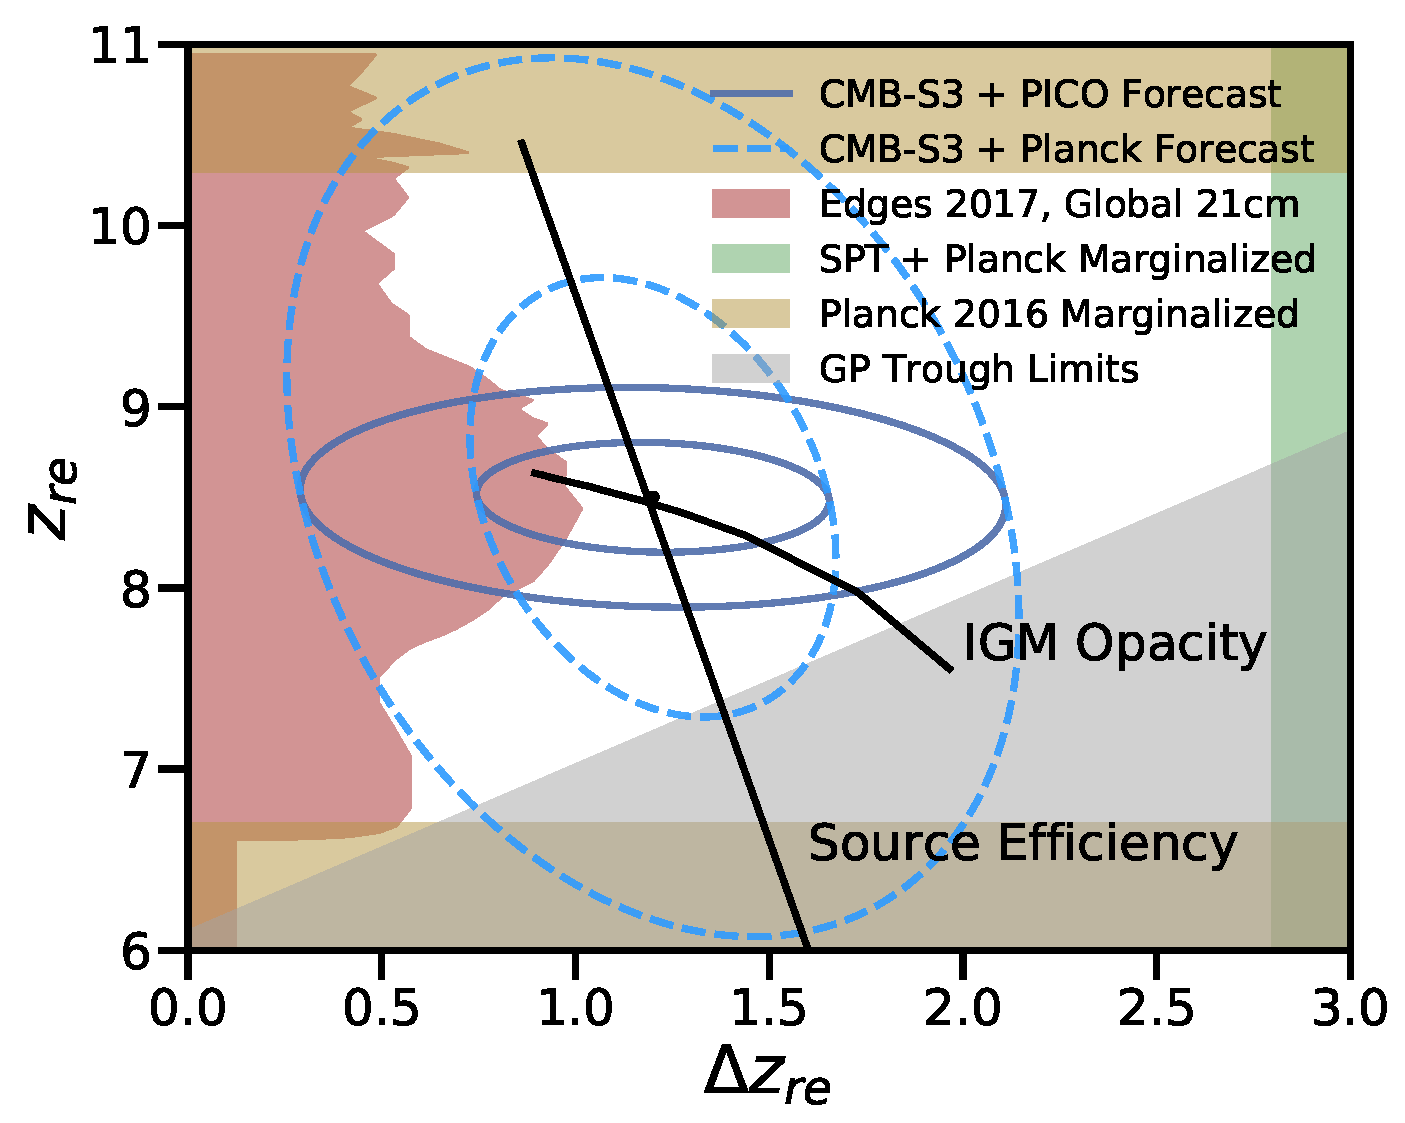
\includegraphics[width=3.0in]{images/Reionization_Contours_zbar_delz_PICO_NEW.pdf} } }
\hspace{0.in}
\parbox{3.5in}{
\caption{\label{fig:ReionizationPICO} Summary of constraints on the mean redshift and duration of reionization. The forecasts show 68\% and 95\% confidence-level contours for PICO combined with CMB-S3 experiments and Planck combined with CMB-S3 experiments (dark blue and dashed blue, respectively). The solid black lines illustrate how the IGM opacity and source efficiency model parameters map onto this parameter space. The forecasted PICO constraints are compared to: current exclusion limits for the mean redshift of reionization from Planck, shown by the yellow bands \citealp{planck2018:parameters}; recent exclusion limits from the global 21 cm signal measured by EDGES, shown with the red band \citealp{edges2017}; exclusion limits from measurements of the Gunn-Peterson trough from fully absorbed Lyman$\alpha$ in quasar spectra, shown by the grey band \citealp{Fan2006}; exclusion limit on the duration of reionization from Planck and SPT data, shown by the green band \citealp{planck_reio:2016}.} }
\vspace{-0.1in}
\end{figure}

In addition to these signals, reionization also leaves specific non-Gaussian signatures in the CMB.  In particular, patchy reionization 
induces non-trivial 4-point functions in both temperature~\citep{SmithFerraro2017} and polarization~\citep{DvorkinSmith2008}.  The 
temperature 4-point function can be used to separate reionization and late-time kSZ contributions.  Combinations of temperature and 
polarization data can be used to build quadratic estimators for reconstruction of the patchy $\tau$ field, analogous to CMB lensing 
reconstruction.  These estimators generally require high angular resolution, but also rely on foreground-cleaned CMB maps.  Thus, 
while PICO alone may not enable high S/N reconstructions, its high-frequency channels --- which have better than 2 arcmin 
resolution and observe at frequencies that have yet to be demonstrated from the ground --- will enable these estimators to be 
robustly applied to ground-based CMB data sets, a strong example of ground-space complementarity.
\comor{if pico is complementarity by {\it only} providing foreground maps at sufficiently high resolution, I think we should move 
this to the 'complementarity'. It is not a direct science goal or outcome.}

% JCH: I checked the Smith-Ferraro 4-pt estimator, and PICO does not have sufficient resolution to do this (see Fig. 3 of https://arxiv.org/pdf/1803.07036.pdf )

\comor{The Sections below need to be rearranged to match other Science Objective(s) from the STM, but to also relay the breadth of science reachable by PICO, even if those goals are not in the STM.}

{\bf Structure Formation via Gravitational Lensing}

Measurements of the CMB reveal structure imprinted not only at the early time of recombination, but also at nearly every significant ensuing epoch in cosmic history.  In particular the matter between us and the CMB last-scattering surface will deflect the path of CMB photons, a process known as gravitational lensing.  Although the lensing of the CMB is a weak signal, targeted statistical estimators enable its extraction.  Measurements of the lensing signal have rapidly progressed, from the first detections in 2007-8 \citep{2007PhRvD..76d3510S, 2008PhRvD..78d3520H} to the recent $40\sigma$ measurement by the {\it Planck} team \cite{2018arXiv180706210P}.  When applied to a rich dataset such as that expected from the PICO satellite, these estimators will provide a map of all the matter in the Universe in projection, with the most sensitivity at redshift $z \simeq 2$ and down to scales of approximately ten arcminutes.  

Forecasts show that the power spectrum of lensing in the PICO CMB map can be detected at approximately 580$\sigma$ or 650$\sigma$ for the requirement or CBE configurations, respectively.  Such high-S/N measurements are more than an order of magnitude improvement over the current state of the art, obtained by the {\it Planck} team.  The legacy value of the PICO CMB lensing map is immense, as has already been seen with {\it Planck}, particularly through the high-S/N cross-correlation science that will be enabled.  For example, tomographic cross-correlations of the PICO CMB lensing map with samples of galaxies and quasars will yield constraints on structure formation out to redshifts inaccessible to galaxy surveys or galaxy weak lensing maps on their own.  These measurements will yield constraints on dark energy, modified gravity, and neutrino mass (complementary to the neutrino mass inferred from the CMB lensing auto-power spectrum described earlier).  In addition, PICO CMB lensing cross-correlations will yield constraints on the properties of quasars and other high-redshift astrophysics, e.g., a precise determination of the quasar bias (and hence host halo mass) as a function of their properties, such as (non-)obscuration.  We provide further quantitative cross-correlation forecasts below.  Fig.~\ref{fig:lensingNoisePICO} shows per-mode noise curves for the reconstruction of CMB lensing from PICO, demonstrating the wide range of angular scales over which the matter density field will be mapped.  \textbf{Add brief discussion of foreground robustness demonstrated in Fig.~\ref{fig:lensingNoisePICO}}

\begin{figure}
\begin{center}
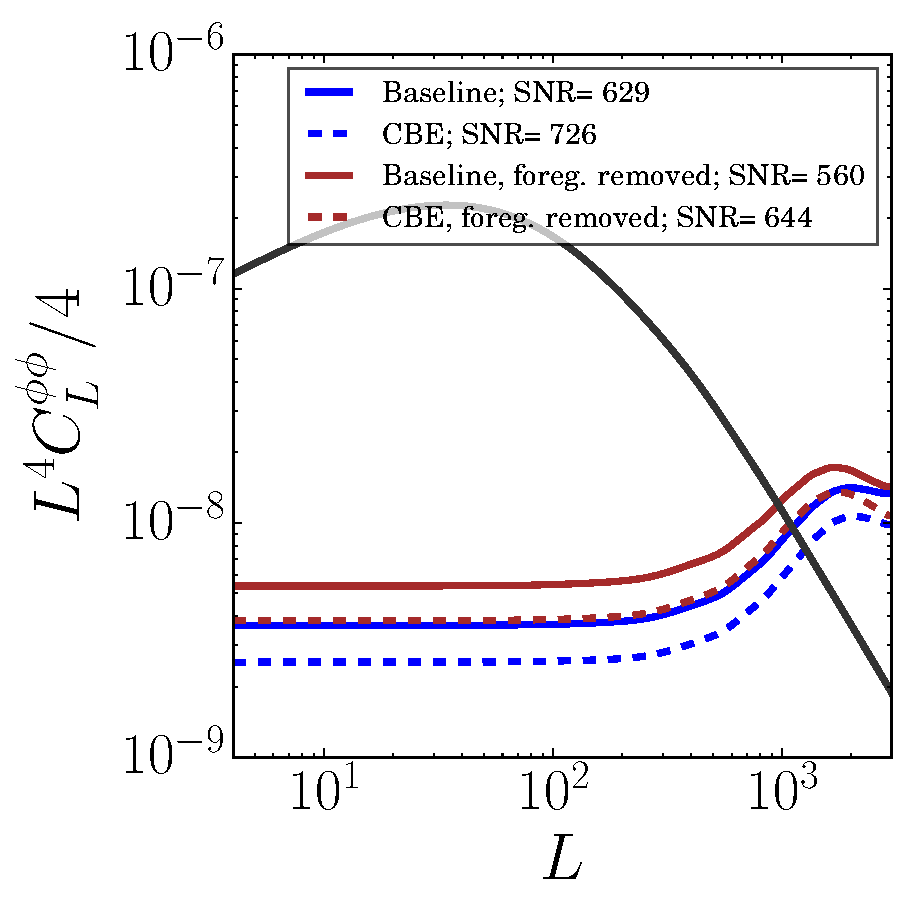
\includegraphics[width=0.6\textwidth]{images/lensingNoisePICO.pdf}
\end{center}
\caption{\label{fig:lensingNoisePICO} Lensing noise curves for various experimental configurations, showing the noise per mode of the reconstructed lensing field.  The signal curve, i.e., the CMB lensing power spectrum, is shown in grey; mapping of the matter density field is possible on scales where the noise curves fall below this signal.  Shown in solid are the performance of the $EB$ polarization estimator, including iterated delensing; this estimator performs best on large angular scales.  On smaller angular scales the temperature ($TT$) estimator shows the best performance. The associated signal to noise ratio for the lensing power spectrum is 570 for the 'requirement' configuration and 650 for the 'CBE' configuration. \textbf{Update with foreground-cleaned polarization noise curve(s) to demonstrate robustness}}
\end{figure}

Lensing breaks the highly symmetric configuration of primordial density fluctuations appearing as $E$ modes on the sky, turning some of these into $B$ modes.  If not accounted for, this effect yields a noise floor on the large-scale $B$ modes that can be measured from the early Universe.  However, maps of $E$ modes and of the lensing field, both of which will be obtained with PICO data, can be used together to create a template for these lensed $B$ modes.  This template can then be subtracted from the measured $B$ modes to obtain improved performance, in a process known as ``delensing'' \citep{2004PhRvD..69d3005S,2012JCAP...06..014S}.  Forecasts show that up to 80\% of the lens-induced $B$ mode power can be removed in the 'requirement' configuration, with this number becoming 85\% for the current best estimate.  

\textbf{To be added:}

\textbf{- CMB halo lensing forecast (Jim, Jean-Baptiste)}

\textbf{- Cross-correlation forecast (Marcel)}


{\bf Physics of Galaxy Formation via the Sunyaev-Zel'dovich (SZ) Effects}

Not all CMB photons propagate through the universe freely; about 6\% are Thomson-scattered by free electrons in the intergalactic medium (IGM) and intracluster medium (ICM). These scattering events leave a measurable imprint on CMB temperature fluctuations, and they contain a wealth of information from how structure grows to the thermodynamic history of baryons. A fraction of these photons are responsible for the Sunyaev--Zel'dovich effects~\citep{SZ1969,SZ1972}. The thermal SZ effect (tSZ) is the increase in energy of CMB photons due to scattering off hot electrons. This results in a spectral distortion
%, proportinal to the electron pressure,
 of the CMB blackbody that corresponds to a decrement in CMB temperature at frequencies below 217 GHz and an increment at frequencies above. The kSZ effect is the Doppler shift of CMB photons Thomson-scattering off free electrons that have a non-zero peculiar velocity with respect to the CMB rest frame. 
%This produces small shifts in the CMB temperature proportional to the radial velocity of the object and its optical depth.
The amplitudes of the tSZ and kSZ signals are proportional to the integrated electron pressure (tSZ) and momentum (kSZ) along the line of sight, respectively.  They thus contain information about the thermodynamic properties of the IGM and ICM.
%since their magnitudes are proportional to the integrated electron pressure (tSZ) and momentum (kSZ) along the line of sight.
The tSZ effect can be used to measure ensemble statistics of galaxy clusters, which contain cosmological information, as well as to provide uniform cluster samples for galaxy formation studies in dense enviroments.
%
%\item Cosmological parameters from the abundance of tSZ-detected clusters and statistics of component-separated tSZ maps.
%\item Thermodynamic properties of galaxies, groups, and clusters from combined tSZ and kSZ cross-correlation measurements.
%\item Measurements of peculiar velocities, which are powerful cosmological probes on large scales, through the kSZ effect.
%\item Patchy reionization which imprints the CMB through higher order moments of the kSZ effect.

{\bf Galaxy Clusters}

%Through the tSZ PICO will produce a large all sky catalog of 

Galaxy clusters found via the tSZ  effect provide a well-defined sample with a simple-to-model selection function. Sample of clusters such as these are easy to use for cosmological inferences and studies of galaxy evolution in dense environments. 
Points to still hit.
High z sample,
Numbers -- Nick and Jim should cross-check,
most massive cluster all over the whole sky,
Cosmology.

{\bf Compton-$y$ map and tSZ auto-power spectrum}

In addition to finding individual clusters, multifrequency CMB data also allow the reconstruction of full-sky maps of the thermal SZ signal (Compton-$y$ maps) via foreground removal algorithms similar to those used to obtain cleaned maps of the CMB.  With its extremely low noise and broad frequency coverage, PICO will yield a definitive Compton-$y$ map over the full sky, with high S/N down to angular scales of a few arcminutes.  We quantify this expectation by reconstructing the Compton-$y$ field using the needlet internal linear combination (NILC) algorithm~\cite{Delabrouille2009} applied to sky simulations generated with the \planck sky model, with maps at all PICO frequencies (with appropriate noise added).  The error bars on the reconstructed tSZ power spectrum are shown in Fig.~\ref{fig:PICO_tSZ_PS}, in comparison to current measurements.  The total $S/N = 1270$ for the PICO CBE configuration, with the PICO requirements configuration only $\approx 10$\% lower.  This is nearly two orders of magntiude larger than the current S/N from \planck.

Extremely strong constraints on models of astrophysical feedback will be obtained from the analysis of the PICO $y$-map, both from its auto-poewr spectrum and from cross-correlations with galaxy, group, cluster, and quasar samples.  Like the CMB lensing map described above, the legacy value of the PICO $y$-map will be immense.  As an example, we forecast the detection of cross-correlations between the PICO $y$-map and galaxy weak lensing maps constructed from LSST and WFIRST data.  Considering the LSST ``gold'' sample with a source density of 26 galaxies/arcmin${}^2$ covering 40\% of the sky, we forecast a detection of the tSZ -- weak lensing cross-correlation with S/N = 3000.  At this immense significance, the signal can be broken down into dozens of tomographic redshift bins, yielding a precise breakdown of the evolution of thermal pressure over cosmic time.  For PICO and WFIRST (assuming 45 galaxies/arcmin${}^2$ covering 5.3\% of the sky), we forecast S/N = 1100 for the tSZ -- weak lensing cross-correlation.  The WFIRST galaxy sample extends to higher redshift, and thus this high-S/N measurement will allow the evolution of the thermal gas pressure to be probed to $z \approx 2$ and beyond, the peak of the cosmic star formation history.  These transformative measurements will revolutionize our understanding of galaxy formation and evolution by distinguishing between models of feedback energy injection at high significance.  Additional cross-correlations of the PICO $y$-map with quasar samples, filament catalogs, and other large-scale structure tracers will further demonstrate its immense legacy value.

\begin{figure}
\begin{center}
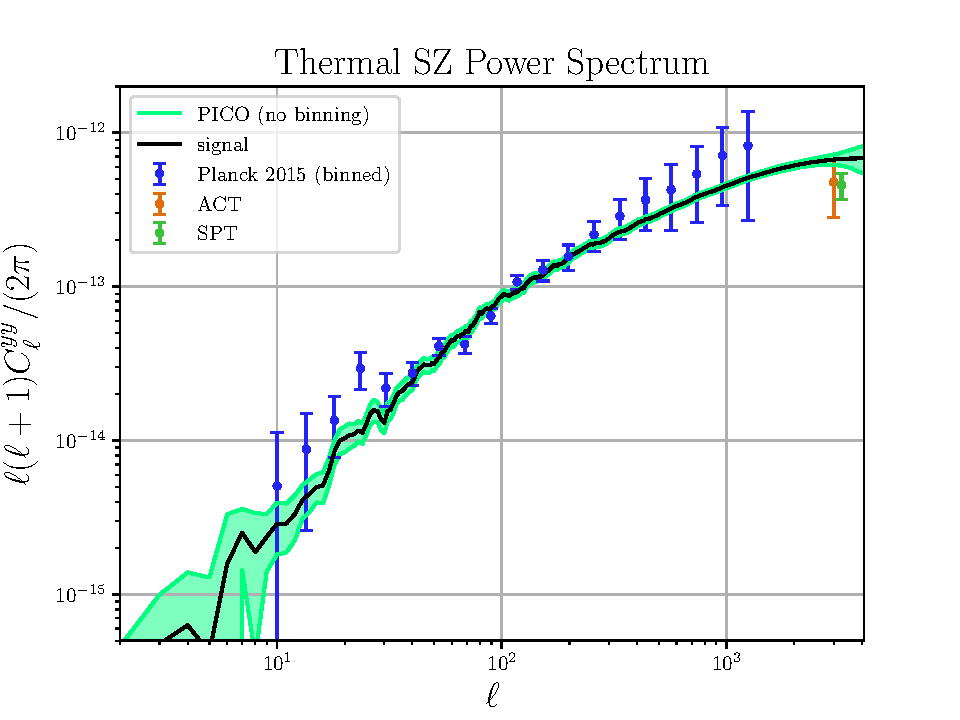
\includegraphics[width=0.8\textwidth]{images/PICO_tSZ_PS_plot.pdf}
\end{center}
\caption{\label{fig:PICO_tSZ_PS} Constraints on the tSZ power spectrum from PICO and current data.  The black curve shows the simulated tSZ power spectrum signal.  The light green shaded region shows the error bars for PICO at each multipole, i.e., with no binning, as determined from NILC analysis of full-sky simulations.  The blue points show the current constraints from Planck, which have been averaged into broad multipole bins.  The orange and dark green points show the constraints from ACT and SPT, respectively, at a single multipole of $\ell=3000$.  The overall PICO $S/N = 1270$, nearly two orders of magnitude larger than current measurements.}
\end{figure}


\end{document}

%\begin{figure}[!htb]
%\centering
%
\includegraphics[width=4cm]{images/example}
%\caption{example}
%\label{fig:im_3}
%\end{figure}


\subsection{Galactic Science}
\documentclass[PICOReport.tex]{subfiles}

\begin{document}

\planck\ enabled an immense step forward in Galactic astrophysics~\citep{Planck2018:XII}. With 7 full sky polarization maps at frequencies between 30 
and 353~GHz and a highest resolution of 5\arcmin, \planck\ provided entirely new and surprising data about the structure of the ISM; the data have a lasting legacy for the foreseeable future. PICO will provide an even greater leap forward, with 21 polarization maps, each much deeper than \planck's, and with the highest resolution being 5 times finer (Fig.~\ref{fig:allsky}). Such a data set can only be obtained from space. 
%\comblue{These data will complement a rich array of other polarization observations forthcoming in the next decade including stellar polarization surveys to be combined with Gaia astrometry, and synchrotron observations with the SKA (and its precursors) to measure Faraday rotation at radio wavelengths.} 
While the PICO data will likely provide many new insights and surprises, we focus here on two particularly important science objectives that are integral to NASA's science goal to explore how the Universe evolved and can only be addressed by the PICO dataset. These objectives relate to the structure and evolution of the Milky Way. \\
%
%Observations of Galactic polarization are a highlight and a lasting legacy of the {\em Planck} space mission. Spectacular images combining the intensity of dust with the texture derived from polarization data have received world-wide attention and have become part of the general scientific culture\comor{literature?} \citep{PlanckI2015}. Beyond their popular impact, the Planck polarization maps represented an immense step forward for Galactic astrophysics \citep{Planck2018:XII}. We expect an even greater leap forward from PICO based on the higher angular resolution dust polarization images obtained with the balloon experiment BLASTPol.  \comor{review sentence} PICO will provide all-sky maps of dust polarization at higher resolution than BLASTPol and with significantly higher sensitivity than {\em Planck} (Fig.~\ref{fig:allsky}.) \comor{reference to older figure?} Such a data set can only be obtained from a space mission. 
%Planck made hundreds of thousands of measurements of magnetic field orientation across the sky; with PICO we expect $\sim1.5\times 10^8$ independent measurements in the 799 GHz band alone.
%The data will complement a rich array of polarization observations including stellar polarization surveys to be combined with Gaia astrometry and synchrotron observations with the SKA (and its precursors) to measure Faraday rotation at radio wavelengths. Here, we focus on two crucially important Galactic science measurements that require PICO. \comor{align questions with headers?}
%
(1) {\em Test Composition Models of Interstellar Dust:} 
Less than one thousandth of a millimeter in size, dust grains are intermediate in the evolution from atoms and molecules to large solid bodies such as comets, asteroids, and planets. Encoded in the composition of dust are the pathways through which grains formed and grew. Dust grains also participate directly in interstellar chemistry, e.g., by catalyzing the formation of H$_2$ and organic molecules on their surfaces, in ways that depend upon their chemical makeup. Thus, the composition of dust grains is an essential aspect of the chemical evolution of interstellar matter from the formation of complex molecules in space to the growth of planets. Through vastly improved spectral characterization of Galactic polarization, the PICO data will discriminate among models of Galactic dust composition to elucidate the chemical evolution of the Galaxy. The data will inform methods to separate diffuse dust emission from cosmological signals of interest (SO6). \\
%\comor{can you please connect to 'galactic structure and evolution' (see example below)? also connect to foregrounds for B-mode if you think appropriate, or can leave this connection to later} \\
%
(2) {\em Determine how magnetic fields affect the processes of molecular cloud and star formation:}
Stars
%, the compact and most luminous constituent of galaxies,
are formed through interactions between gravitational and magnetic fields, turbulence, and gas over more than four orders of magnitude of spatial scales. However, the role magnetic fields play in the large scale structure of the diffuse \ac{ISM} and in the observed low star-formation efficiency has eluded answer because of dearth of data. 
By virtue of the strong dynamical coupling of dust and gas and the systematic alignment of dust grains with magnetic fields, PICO's dust polarization measurements will for the first time probe the large scale Galactic magnetic field with resolution to trace the role of magnetic fields through the entirety of the star formation process (SO7). 
%\comor{We should probably switch the order of these and the sections below to match with the STM; or switch the STM? DC- I would vote for switching the STM here.}

%By virtue of the strong dynamical coupling of dust and gas, and the systematic alignment of dust grains with magnetic fields, dust polarization probes magnetic fields in the cold and warm neutral phases of the diffuse \ac{ISM} (which contains the bulk of the \ac{ISM} gas mass and turbulent energy) down to the scale of molecular clouds (which are where stars form). \comor{long and confusing sentence} PICO will measure polarization across this broad range of scales to trace the role of magnetic fields through the entirety of the star formation process. 

%If the magnetic fields are sufficiently strong, they can prevent the gravitational collapse of gas across magnetic field lines and can slow down or limit the processes of star and planet formation.
%In the diffuse ISM the neutral phase of the interstellar medium contains the bulk of the gas mass 
%and of its turbulent kinetic energy.
%
%
\begin{figure}
    \centering
    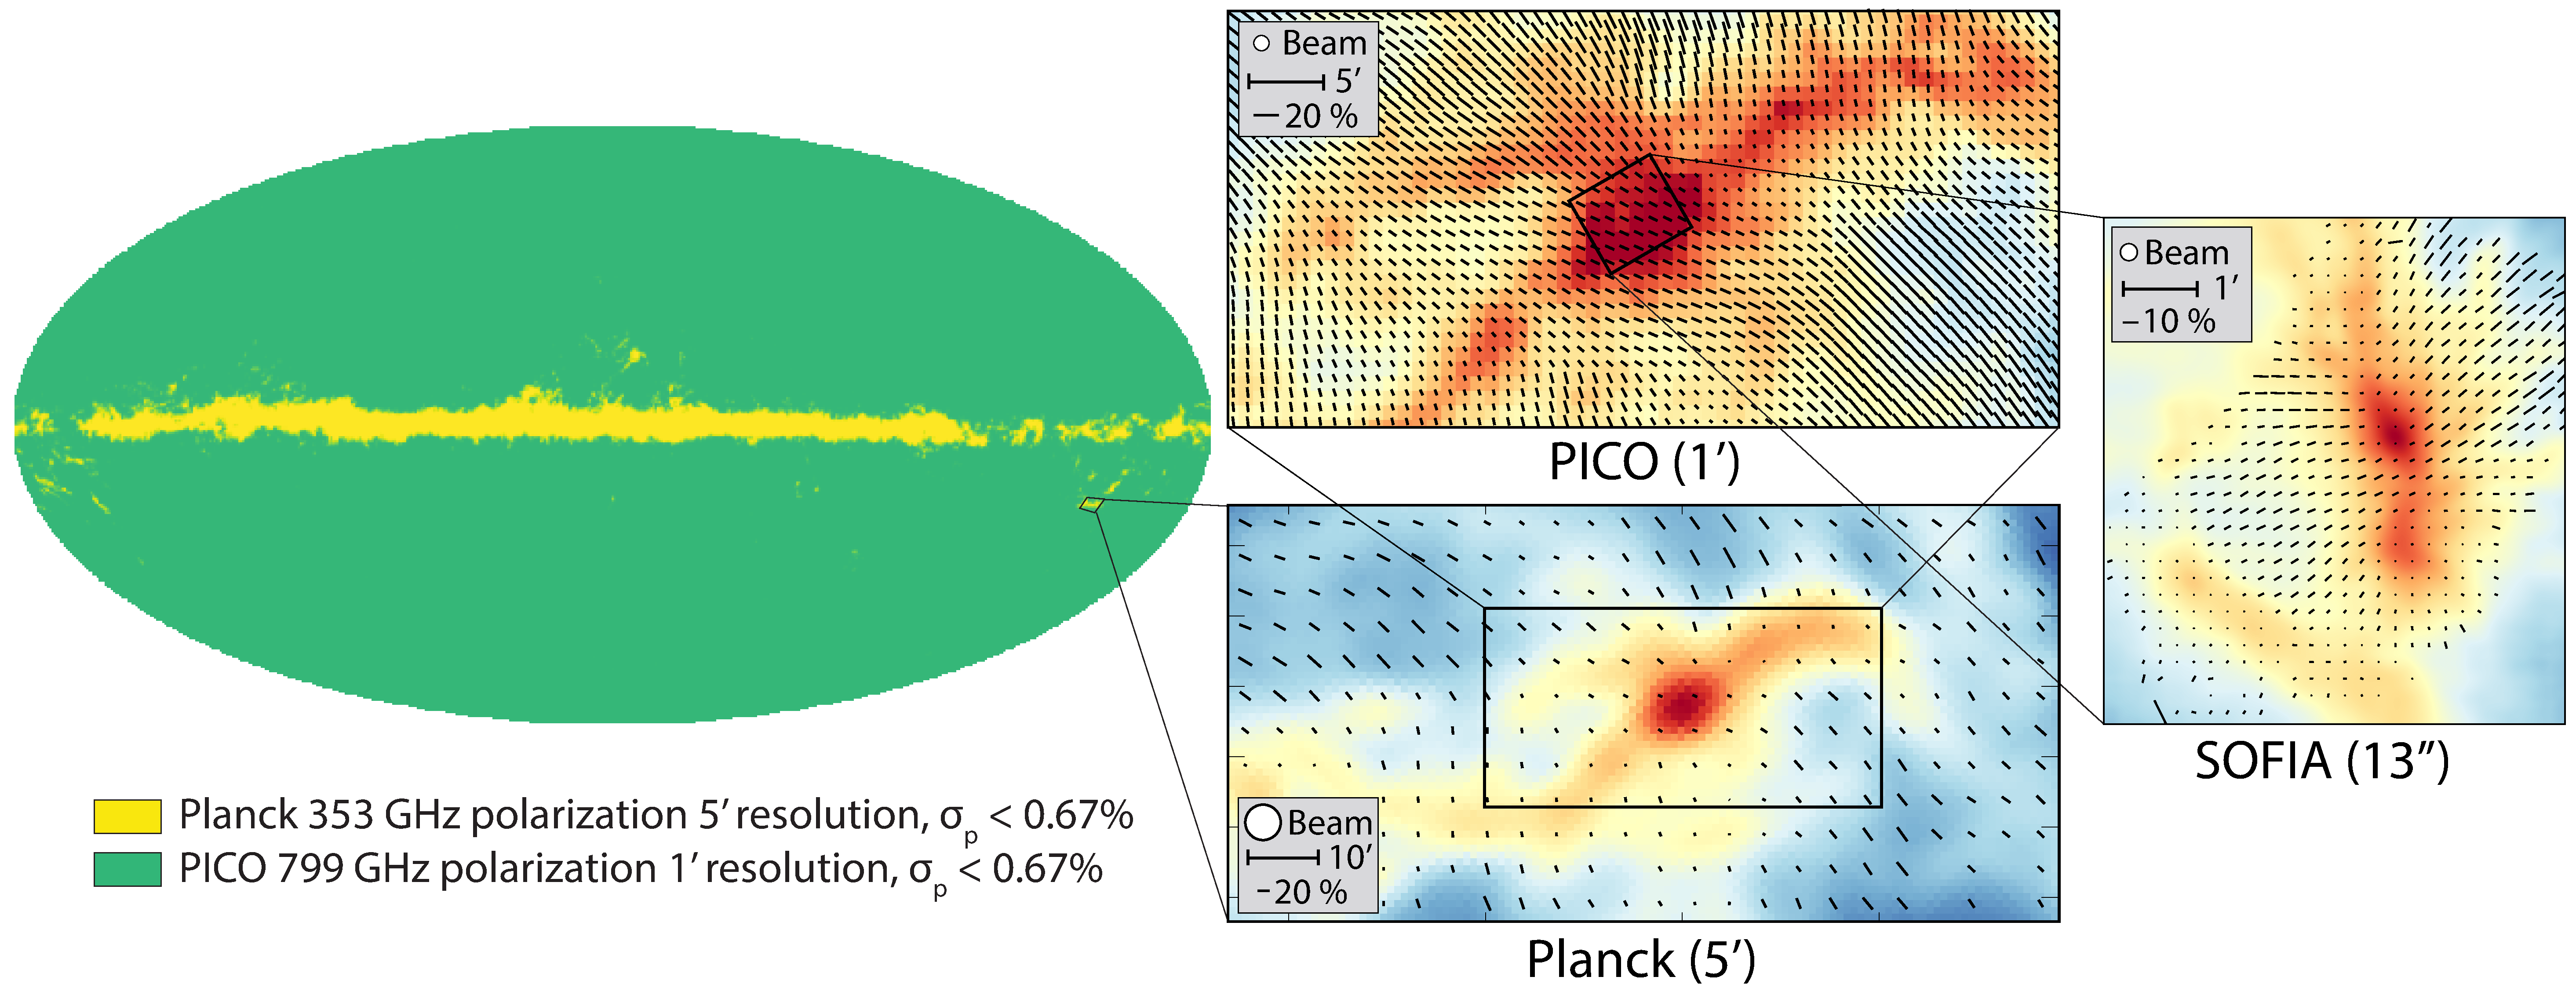
\includegraphics[width=6.5in]{galsci_fig_v4.pdf}
    \caption{\captiontext  \planck 's 353~GHz polarization map gave a resolution of 5\arcmin~and sensitivity to polarization intensity of $\sigma_{p} < 0.67\%$ over a small portion of the sky (left, yellow).  At 799 GHz, the PICO baseline mission will give a polarization map of the {\it entire sky} and with 5 times higher resolution (left, green). The \planck~map of the Orion region overlaid with vectors that are aligned with the inferred magnetic field (lower panel), and a simulated PICO observation (upper panel) illustrate the leap in information content (vector lengths are proportional to polarization fraction). With this map, and maps at many other frequencies that \planck~did not have, PICO will characterize Galactic magnetized turbulence at scales spanning the diffuse ISM down to dense star forming cores, which will be mapped with high-resolution polarimetry by instruments such as HAWC+/SOFIA \citep{Chuss2018} (right panel) and the Atacama Large Millimeter Array \citep[ALMA,][]{Bacciotti2018ApJ}.}
    \label{fig:allsky}
\end{figure}

\noindent{\bf (1) Test Composition Models of Interstellar Dust} \\
Strong extinction features at 9.7 and 18~$\mu$m indicate that much of interstellar dust is in the form of amorphous silicates while features at 2175\,\AA, 3.3~$\mu$m, and 3.4~$\mu$m attest to abundant hydrocarbons. It is unknown, however, whether the silicate and carbonaceous materials coexist on the same grains or whether grains of each composition grow through distinct, parallel pathways dictated by their surface chemistry. 
%If there are indeed multiple grain populations, this will induce additional challenges for modeling the emission from interstellar dust in both total intensity and polarization at levels relevant for B-mode science at all angular scales~\citep{Hensley2018}. 

%\comor{The last sentence implies that the issue of multiple grain populations is only important for CMB B-mode science. Is it? Is it not important on its own right, because it is important to know what dust is made of? This is the missing connection to the broader picture: why do we care about dust?}

Some data suggest that the populations are distinct. Spectropolarimetry of dust extinction reveals robust polarization in the 9.7\,$\mu$m silicate feature~\citep[e.g.,][]{Smith2000}, indicating that the silicate grains are aligned with the interstellar magnetic field. In contrast, searches for polarization in the 3.4\,$\mu$m carbonaceous feature have yielded only upper limits, even along sightlines where silicate polarization is observed~\citep{Chiar2006,Mason2007}. These data are consistent with silicate and carbonaceous materials existing on separate grains that have different alignment properties. 
%\comblue{However, the 3.4~$\mu$m feature arises only from aliphatic (chain-like) carbonaceous material, which may not trace all carbon-bearing grains. Additionally, available data are restricted to only a few highly-extincted sightlines that may not typify the entire diffuse \ac{ISM}.}

At odds with the spectropolarimetric evidence from dust extinction are current measurements of the polarization fraction of the far-infrared dust emission with \planck~\citep{Planck_Int_XXII} and BLASTPol~\citep{Ashton2018}. They show little to no frequency dependence, whereas substantial frequency dependence would be expected if two components with distinct polarization properties were contributing to the total emission. 
%\comblue{However, current uncertainties are relatively large and the BLASTPol data are from only high density sightlines that may not be representative of the diffuse \ac{ISM}. }

With excellent polarization sensitivity, even in diffuse regions, PICO will provide a definitive test of the two component paradigm \citep{Meisner2015}. 
%\comblue{To assess PICO's ability to discriminate models quantitatively, we employed the analytic two component dust model of Meisner et al.~\cite{Meisner2015}, which provided a better fit to IRAS and \planck\ data than one component models. We ran 1000 simulations with different combinations of polarization fractions of the two components. We used PICO baseline noise levels, frequency bands at and above 107~GHz, and binned the simulated data in 7.9$^\prime$ pixels, matching the beam of the PICO 107~GHz band.} 
In this case, the PICO baseline mission will determine the intrinsic polarization fractions of each of the two components to a precision of 3\%. With this level of precision the data will validate or reject state-of-the-art dust models~\citep[e.g.][Hensley \& Draine, in prep]{Guillet2018}, test for the presence of additional grain species with distinct polarization signatures, such as magnetic nanoparticles~\citep{Draine2013}, and will be used as a crucial input for the foreground separation necessary to extract cosmological B-mode science. %
%
%\comor{perhaps here talk about B-mode foregrounds and connect to AME?}
%\comor{give a sentence about AME: An additional emission of unknown origin has been detected in ... GHz. It is called AME ... The \ac{AME} is an important foreground in the 20-60~GHz region, but at this time the level of polarization of the AME remains controversial~\cite{Dickinson2018b}, and the spectral profile has only been well-characterized in very bright regions. } 

``Anomalous Microwave Emission (AME)'' is a component of Galactic emission peaking in the 20-30~GHz range that has been tentatively identified with small, rapidly-spinning dust grains.\citep{dickinson/etal:2018} As only upper limits have been placed on its polarization, its role as a foreground for B-mode science remains unclear. Given the present uncertainty on its physical origin and SED variability, even small levels of polarization could prove challenging. However, PICO will finely sample the AME SED with its bands at 21, 25, 30, 36, and 43 GHz. Combined with ground-based maps at lower frequencies \citep[e.g., C-BASS][at 5~GHz]{Dickinson2018a}, PICO will efficiently separate the AME from synchrotron and free-free emission and either detect or place stringent upper limits on its polarization.
%the PICO data set will utilize the distinct spectral dependence of synchrotron ($I_{\nu} \propto {\nu}^{-1}$), free-free ($I_{\nu} \propto {\nu}^{-0.1}$), and \ac{AME} to enable reliable component separation. 
Further, the enhanced frequency coverage will enable characterization of systematic changes in the AME SED with interstellar environment and thus elucidate its underlying physics.

\noindent{\bf (2) Determine how magnetic fields affect the processes of molecular cloud and star formation} \\
Stars form out of dense, gravitationally unstable regions within molecular gas clouds, which themselves form through the flow of diffuse, atomic-phase gas to denser regions. Magnetic fields play an important role throughout this process. 

On the largest scales, magnetized turbulence mediates the flow of the gaseous \ac{ISM} from the atomic to the denser, molecular phase. Recent observations suggest that the structure of the diffuse medium is highly anisotropic, and strongly coupled to the local magnetic field~\citep{Clark:2014, Clark:2015, Kalberla:2016, KalberlaKerp:2016}. 
As molecular gas clouds collapse to form stars, magnetic fields can slow the process of star formation by inhibiting movement of gas in the direction perpendicular to the field lines. Observations to date suggest that the outer envelopes of clouds can be supported against gravity by magnetic fields and turbulence, but in dense cores gravity tends to dominate, and so these dense structures can collapse to form stars \citep{Crutcher2010}.  The degree to which magnetic fields affect the formation of molecular clouds, as well as stars within these clouds, is poorly constrained, in large part due to the difficulty of making detailed maps of magnetic fields in the ISM.

%Stars form out of dense, gravitationally unstable regions within molecular gas clouds. The efficiency of this conversion from molecular gas to stars is very low, due to regulation from supersonic turbulent gas motions, magnetic fields, and feedback from young stars \citep{McKee2007}.  Magnetic fields may play an important role in slowing the process of star formation by inhibiting movement of gas in the direction perpendicular to the field lines.  Observations to date suggest that the outer envelopes of clouds can be supported against gravity by magnetic fields and turbulence, but in dense cores gravity tends to dominate, and so these dense structures can collapse to form stars \citep{Crutcher2010}.

%On larger scales, the formation of gravitationally unstable clouds is regulated by the flow of diffuse material into the molecular phase\comor{(?)}, a process that is mediated by magnetized turbulence in the low-density \ac{ISM}. Structure formation in the diffuse \ac{ISM} is poorly understood, but as a precursor to star formation it is crucial to understand what drives molecular cloud formation. Recent observations suggest that the structure of the diffuse medium is highly anisotropic, and strongly coupled to the local magnetic field~\citep{Clark:2014, Clark:2015, Kalberla:2016, KalberlaKerp:2016}. However, the degree to which magnetic fields affect the formation of molecular clouds, as well as stars within these clouds, is poorly constrained, in large part due to the difficulty of making detailed maps of magnetic fields in the interstellar medium.

\noindent$\bullet$ {\bf Formation of Magnetized Molecular Clouds from The Diffuse Interstellar Medium} \hspace{0.1in}
A comprehensive understanding of the magnetized diffuse \ac{ISM} is challenging because of its diverse composition, its sheer expanse, and the multi-scale nature of the physics that shapes it. To understand how matter and energy are exchanged between the diffuse and dense media, it is essential to measure the properties of the magnetic field over more than four orders of magnitude in column density. PICO is unique in its ability to provide the necessary data. \textit{Planck} achieved measurements of the diffuse sky at 60\arcmin\ resolution, resulting in $\sim$30,000 independent measurements of the magnetic field direction.  With 1.1\arcmin~resolution PICO will expand the number of independent polarization measurements to 86,000,000. The data will thus robustly characterize turbulent properties like the Alfv\'{e}n Mach number, $\mathcal{M}_A$, across a previously unexplored regime of parameter space. 

PICO's observations will complement recently completed high dynamic range neutral hydrogen surveys, such as \HI4PI \citep{HI4PI:2016} and GALFA-\hi \citep{Peek:2018}, as well as planned surveys of interstellar gas, most prominently with the Square Kilometer Array (SKA) and its pathfinders. One of the open questions in diffuse structure formation is how gas flows within and between phases of the \ac{ISM}. A planned all-sky absorption line survey with the forthcoming SKA-1 will increase the number of measurements of the \ac{ISM} gas temperature by several orders of magnitude~\citep{McClure-Griffiths2015}. Quantitative comparisons of the \ac{ISM} temperature distribution from SKA-1 and estimates of the magnetic field strength and coherence length scale from PICO will elucidate the role of magnetized turbulence in the flow of matter in the \ac{ISM} from diffuse regions to regions of denser molecular gas.

\noindent$\bullet$ {\bf Formation of Stars within Magnetized Molecular Clouds} \hspace{0.1in}
The role of magnetic field in star-formation is quantified by the ratio of energy stored in magnetic and gravitational fields, and the ratio of energy stored in magnetic field and that stored in turbulence. The first ratio is parameterized through a mass-to-flux ratio $\mu$, and the second
through $\mathcal{M}_A$. 

With full-sky coverage and a resolution of 1.1\arcmin, PICO will map all molecular clouds with better than 1\,pc resolution, out to a distance of 3.4\,kpc.  Extrapolating from the Bolocam Galactic Plane Survey \citep[BGPS,][]{EllsworthBowers2015}, PICO is expected to make highly detailed magnetic field maps of over 2,000 molecular clouds with thousands to hundreds of thousands of independent polarization measurements per cloud. These are the {\it only foreseeable} measurements that will give $\mu$ and $\mathcal{M}_A$ over a statistically significant sample of molecular clouds. \planck , for example, mapped only 10 nearby clouds to a similar level of detail~\citep{Planck:XXXV}. A large sample of clouds is crucial because (1) dust polarization observations are sensitive to only the magnetic field projected on the plane of the sky, and therefore polarization maps will look very different for molecular clouds observed at different viewing angles; and (2) the relative importance of the magnetic field will likely be a function of cloud age and mass. By observing thousands of molecular clouds PICO will determine $\mu$ and  $\mathcal{M}_A$ for different sub-classes of cloud age and mass. 

%To constrain $\mu$ and $\mathcal{M}_A$ we will apply a series of established polarization analysis techniques:
%(1) characterizing the relative orientation of cloud structures and the magnetic field \citep{Soler2013,Chen2016,Soler2017,Planck:XXXV}; (2) making probability distributions functions of polarization measurables \citep{Fissel2016, King2018}; (3) comparing the magnetic field and velocity gradient directions \citep{GonzalezCasanova2017,Yuen2017,Lazarian2018}; and (4) measuring the angular dispersion of the magnetic field  \citep{Davis1951,Chandrasekhar1953, Hildebrand2009,Houde2009}.
%By applying all four techniques to both PICO observations and synthetic polarization maps made from ``observing'' numerical simulations of star formation, we will quantitatively compare theory and observations. PICO's large number of frequency bands will be used to better model the temperature and polarization efficiency of the cloud dust  \citep{Andersson2015}, which can then be used to generate more realistic generation of synthetic observations from simulations for comparison with PICO observations \citep{Seifried2018}. We can then compare the observed magnetization levels derived from the PICO observations to the levels of turbulence derived from molecular gas surveys~\cite{EllsworthBowers2015, Miville-Deschenes2017}, and the efficiency of star formation, measured from near and far-IR observations of dense cores and protostars with {\em Herschel}, {\em Spitzer}, and {\em WISE}. \comor{Why italics? Tim, Qi - please check for uniformity}

%{\em PICO's ability to map thousands of clouds is not possible with any other current or proposed polarimeter}. {\em Planck}, for example, was only able to map 10 nearby clouds to a similar level of detail \citep{Planck:XXXV}. This large sample of clouds is crucial because dust polarization observations are sensitive to only the magnetic field projected on the plane of the sky, and therefore polarization maps will look very different for molecular clouds observed at different viewing angles.  {\em By observing thousands of molecular clouds PICO will determine the role of magnetic fields in star formation as a function of cloud age and mass.}

%
\noindent{\bf Galactic Legacy Science}\\
PICO will also produce legacy datasets that will revolutionize our understanding of how magnetic fields influence physical processes ranging from planet formation to galaxy evolution.  For 10 nearby clouds, which have distances of less than 500 pc, PICO will resolve magnetic fields on scales of 0.1~pc. This is the scale of dense cores and filaments for these clouds, and thus the observations will constrain how magnetic fields on these scales influence the formation of cloud cores.  By comparing the orientation of the core-scale magnetic fields with the orientation and sizes of proto-planetary disks, PICO will probe whether magnetic braking influences the growth of such disks~\citep{allen_2003,li_2014} and provide complementarity to higher angular resolution instruments such as ALMA \citep{Bacciotti2018ApJ} and SOFIA \citep{Harper2018}.
%\comor{isn't ALMA or other instruments better suited for this?}

Key processes in the diffuse ISM, including heat transport \citep{Lazarian:2006}, streaming of cosmic rays \citep{Lazarian:2016}, and magnetic reconnection \citep{Lazarian_Vishniac:1999} are dramatically dependent on the level of magnetization.
PICO addresses this with tens of millions of independent measurements of magnetic field orientation over the entire Galaxy that will enable the study the physics of how magnetic fields are generated through a combination of turbulence and large-scale gas motions \citep{Xu_2018}.
%\comor{that has already been said before, no?}. I think this is more focused on the physics of B field generation, not star formation. 
 %\comor{Not clear what this sentence says}

Finally, PICO observations will create detailed magnetic field maps of approximately 70 nearby galaxies, with more than 100 measurements of magnetic field directions per galaxy. These observations will determine how interaction between large-scale magnetic fields, turbulence, and feedback from previous generations of star formation affect galaxy evolution and star formation efficiency.
%\bibliographystyle{aasjournal}
%\bibliography{galsci.bib}

\end{document}

%\begin{figure}[!htb]
%\centering
%
\includegraphics[width=4cm]{images/example}
%\caption{example}
%\label{fig:im_3}
%\end{figure}


\subsection{Legacy Science}
\documentclass[../PICOReport.tex]{subfiles}

\begin{document}
blah

\begin{figure}[!htb]
\centering

\includegraphics[width=4cm]{../images/example}
 
\label{fig:im_example}
\caption{example}
\end{figure}


\end{document}

\subsection{Foregrounds}

\documentclass[PICOReport.tex]{subfiles}

\begin{document}

%Enumerate the various signals in polarization. Use the frequency band + signals figure. The challenge is to dig out the faintest of all signals, the one due to $r$. This sets the tone for the entire 'signal decomposition' or 'component separation'.  Removing the galactic signal to unmask $r \lesssim 0.001$ is a challenge for all future experiments searching for $r$ at that level, and is a strong advantage of a space platform. The physics of galactic signals suggests complexities in their combined emission properties; the level of this complexity is not known. } 

Diffuse Milky Way emissions dominate the sky's polarized intensity on the largest angular scales; see Figures~\ref{fig:clbb} and ~\ref{fig:pico-channels-and-fg}. Polarized radiation arises primarily from the synchrotron emission of energetic electrons spiralling in the magnetic field of our own Galaxy, and from thermal
emission from elongated interstellar dust grains. Although the levels of these foreground emissions decrease with decreasing angular scales, they can still be considerably brighter 
than the \ac{IGW} peak around $\ell=80$ when averaging over 60\% of the sky. 
In fact, even in the cleanest, smaller patches of the sky, far from the galactic plane and thus relatively low in galactic emissions, their levels are expected to be substantial relative to the \ac{IGW} for $r \lesssim 0.01$, and dominate it for $r \lesssim0.001$. Separating the cosmological and Galactic emissions signals, also called foreground separation, together with control of systematic uncertainties are {\it the} challenges facing any next decade experiment attempting to reach these levels of constraints on $r$.

\begin{figure}[ht]
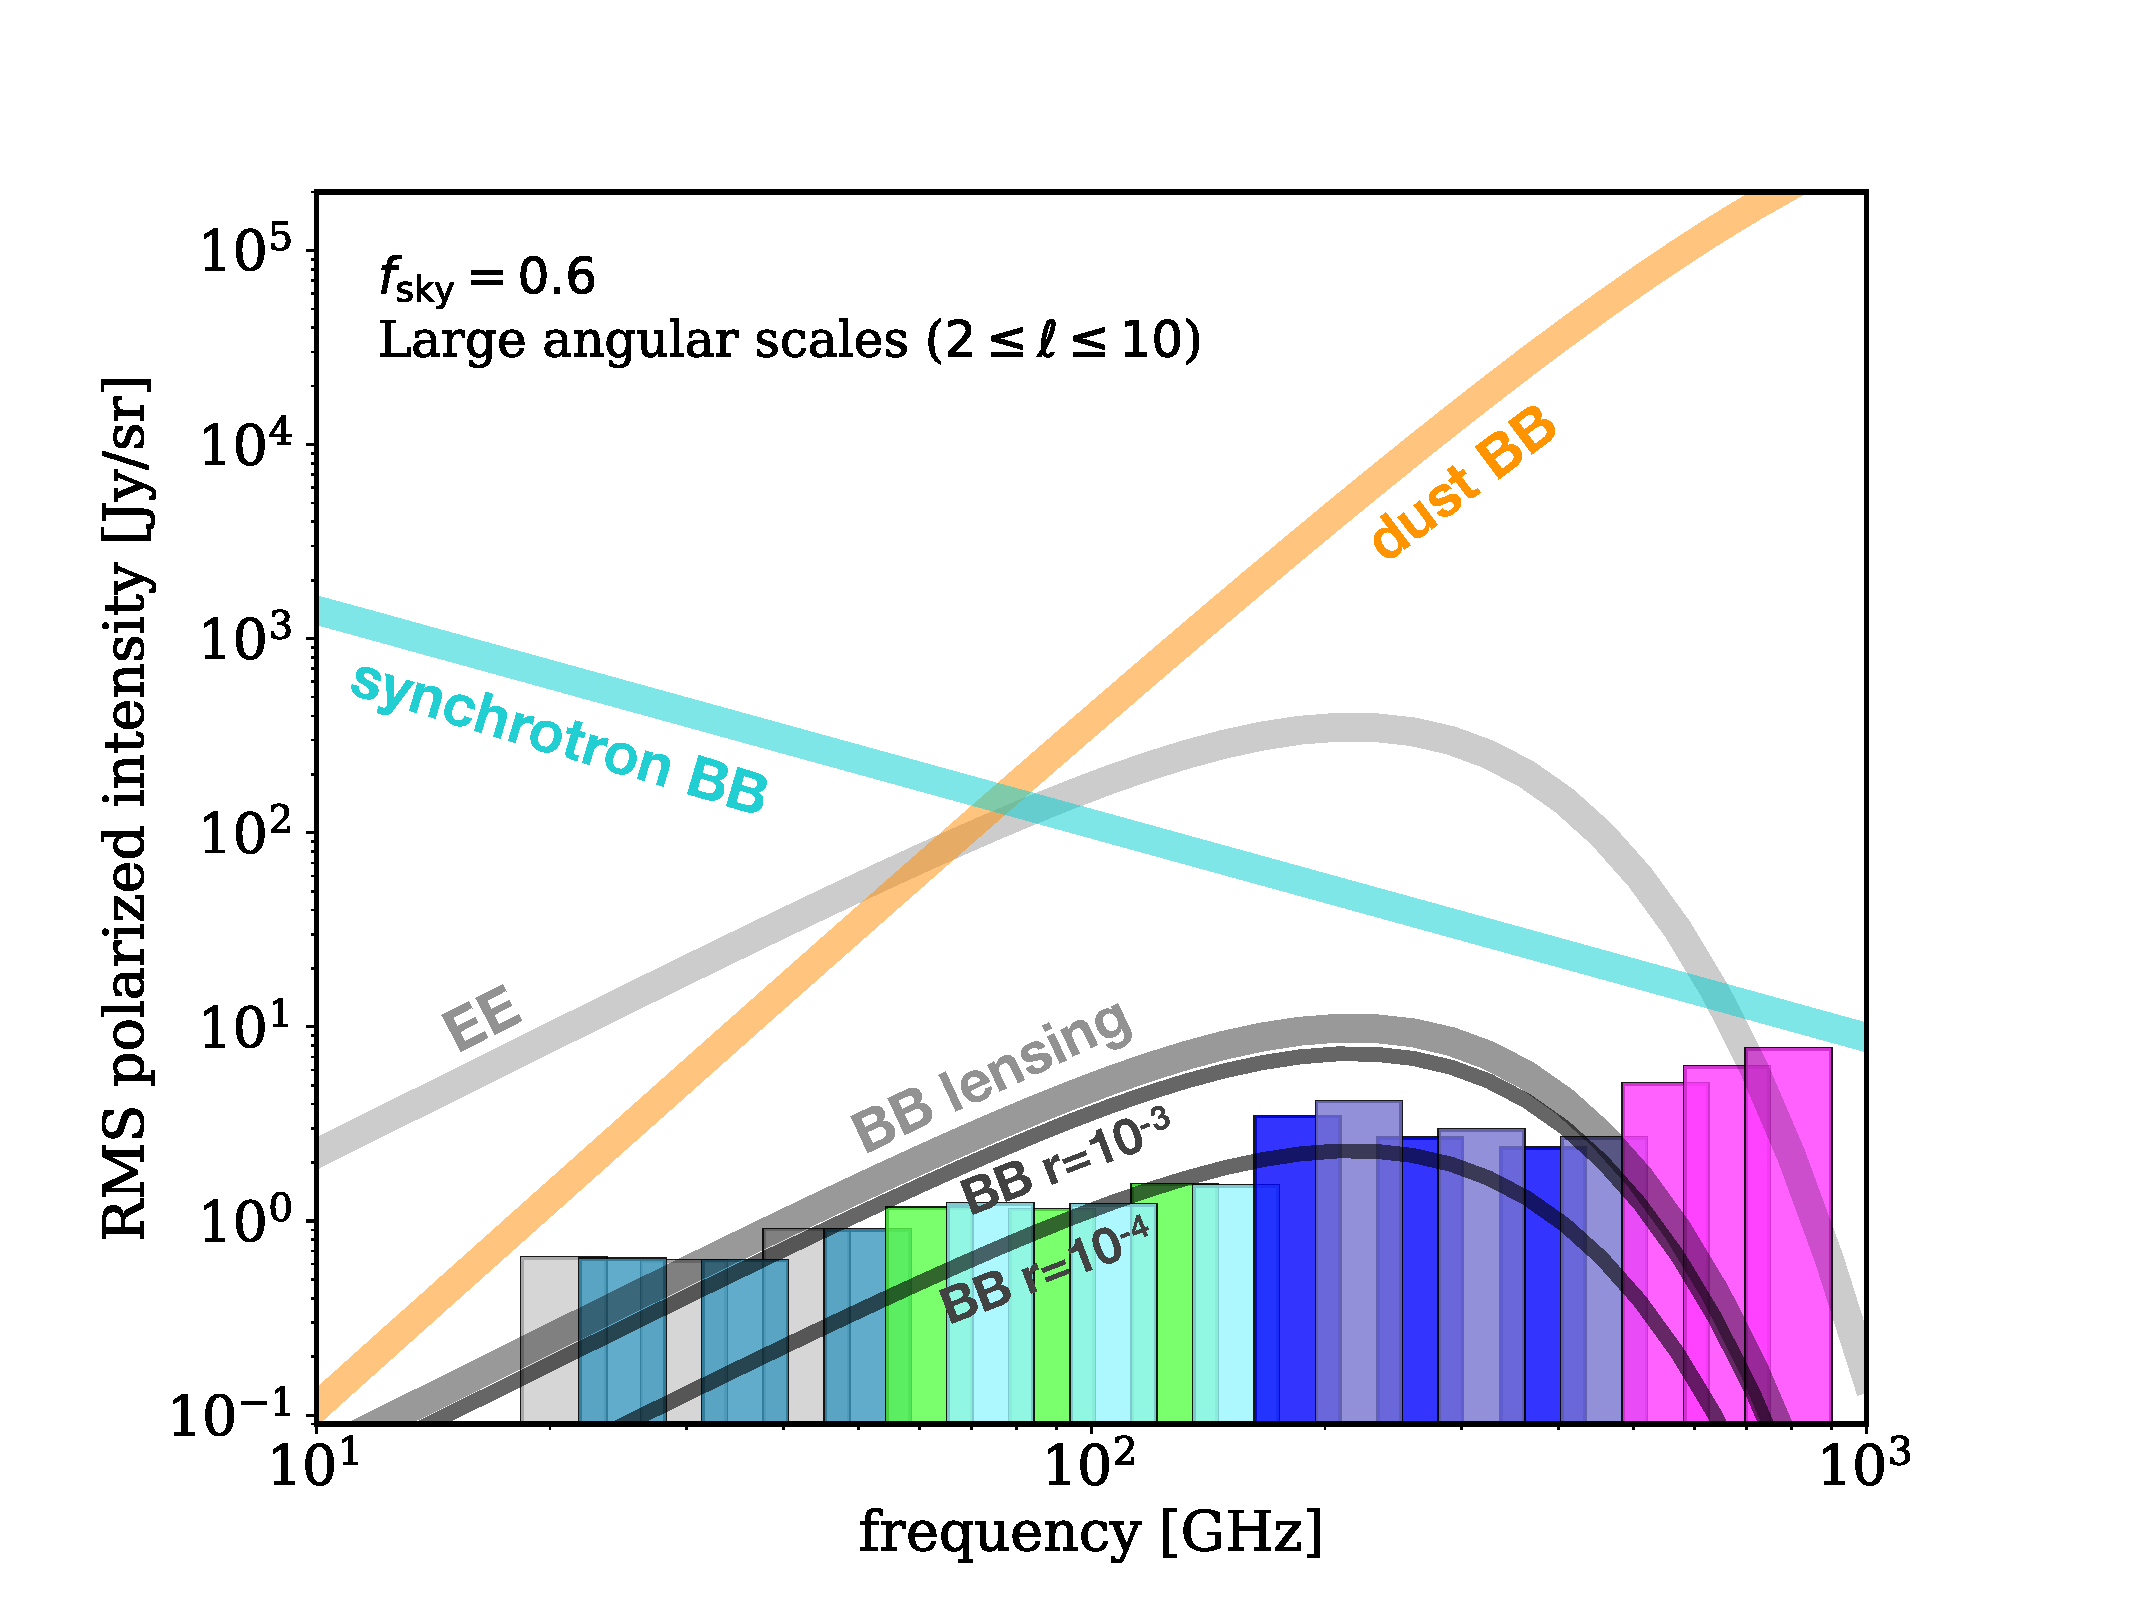
\includegraphics[width=0.49\textwidth]{images/sensitivity_vs_frequency_Jun29th_2018_large.pdf}
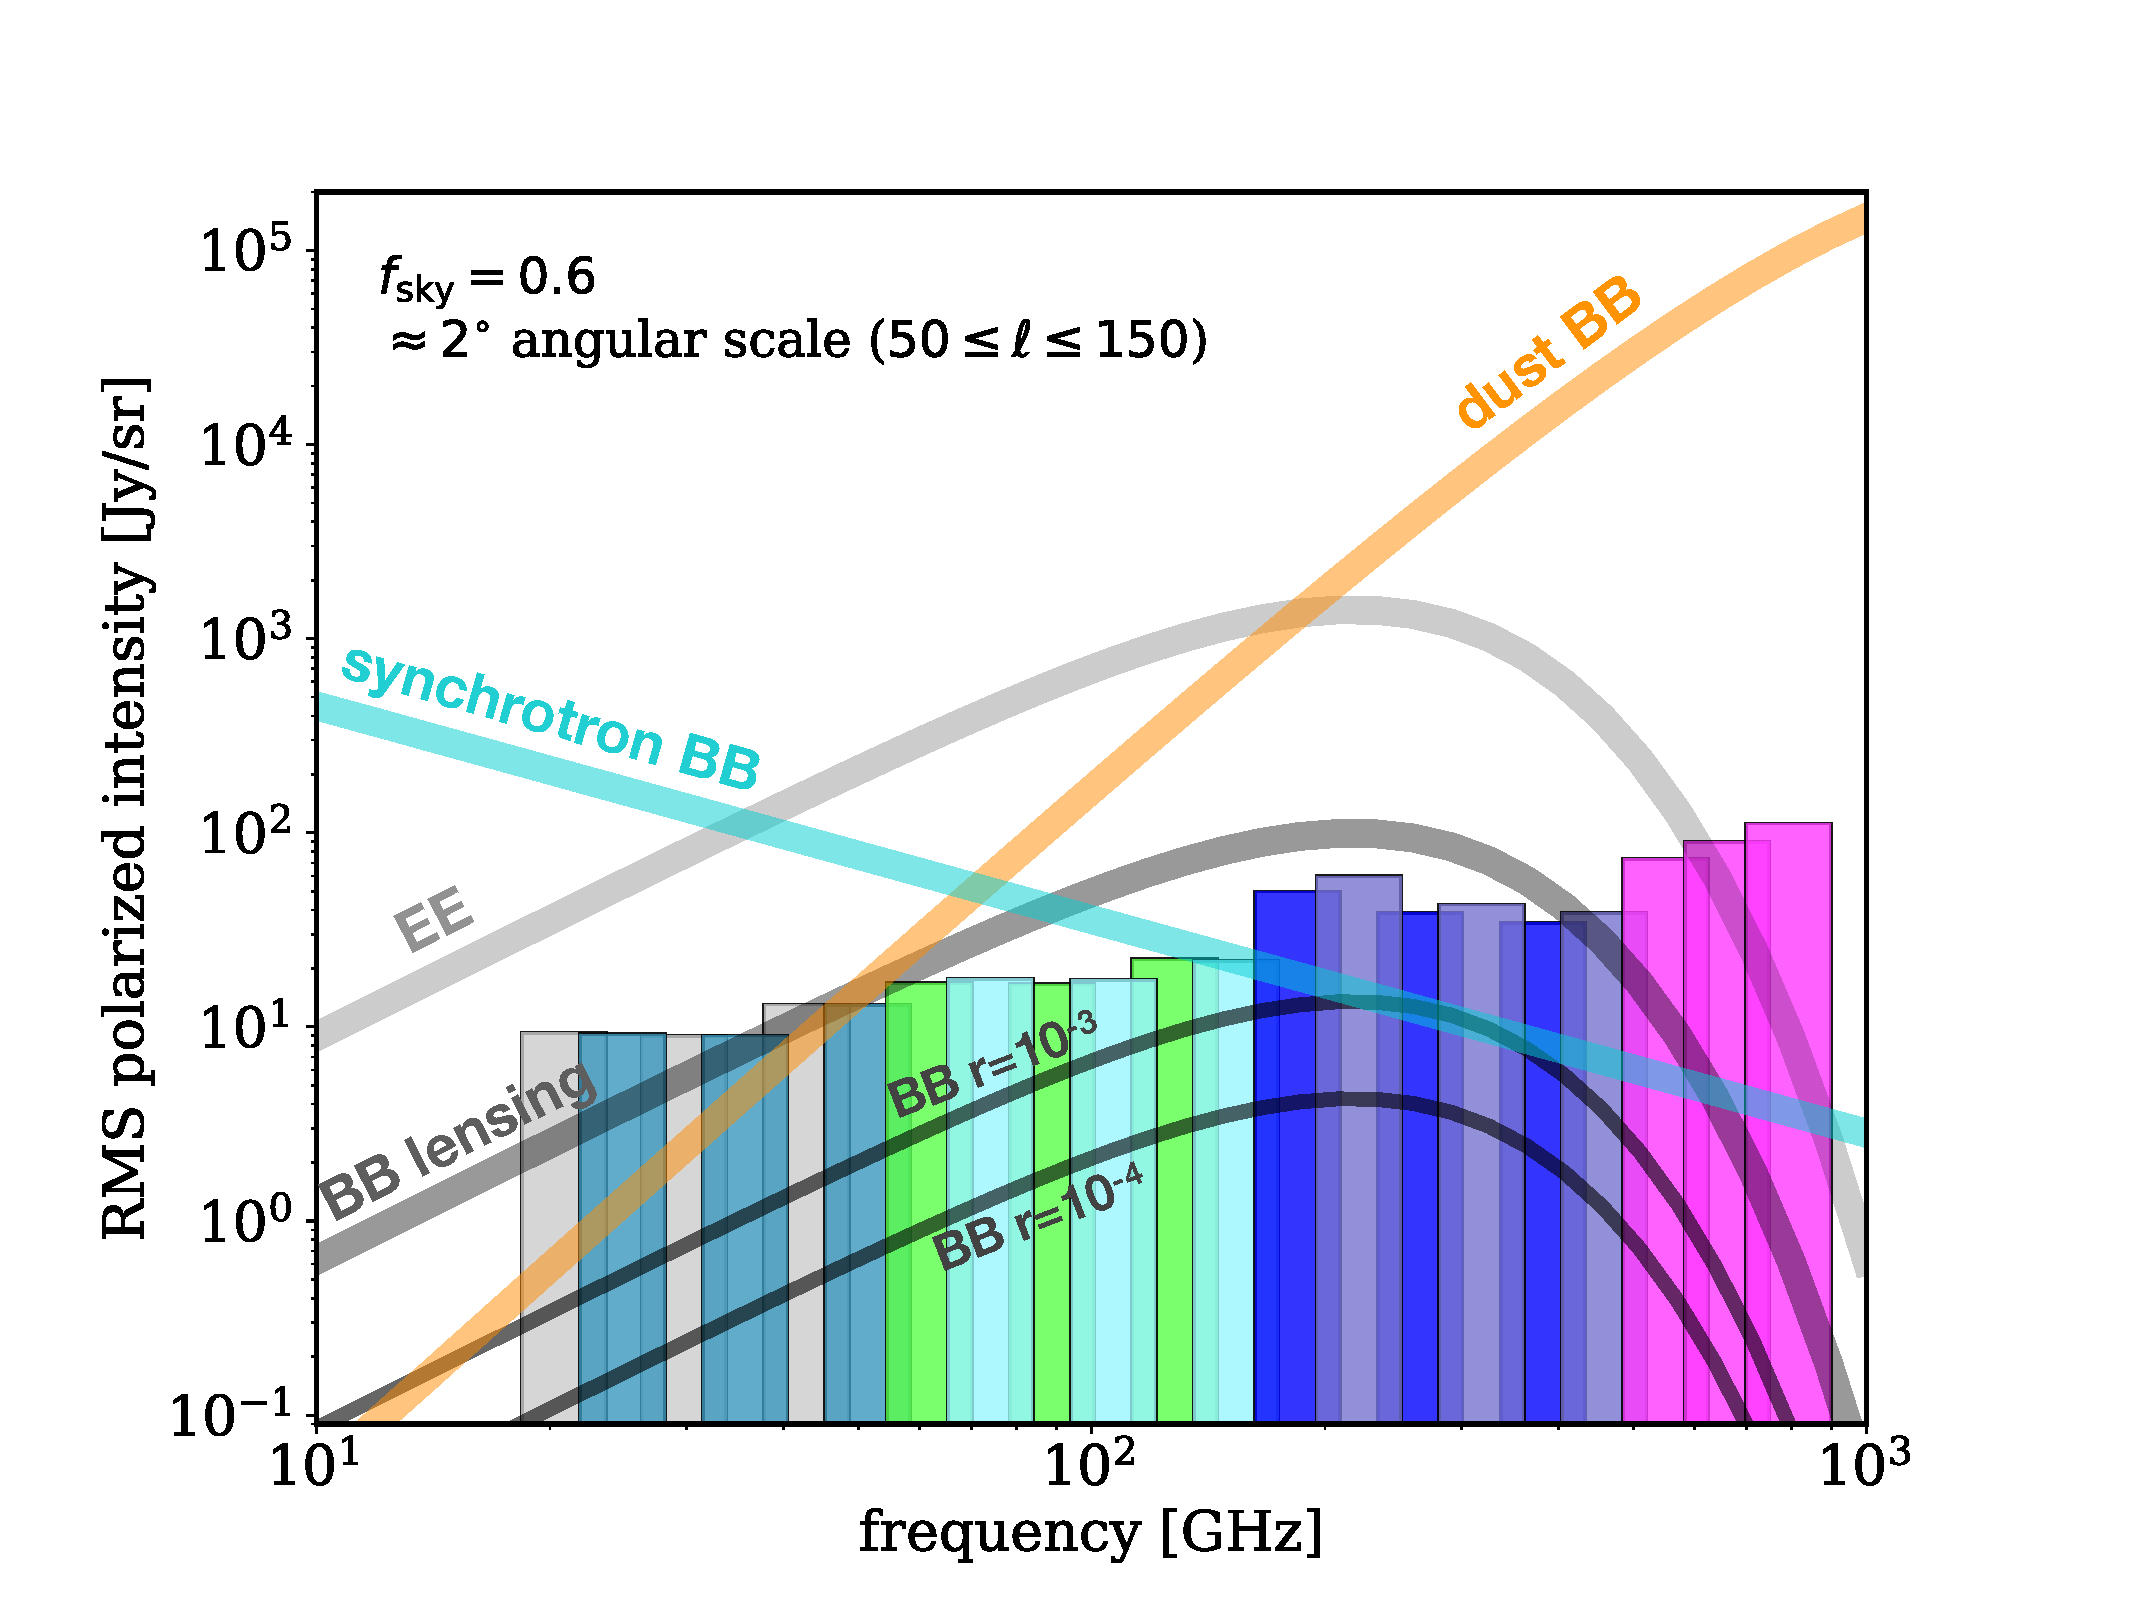
\includegraphics[width=0.49\textwidth]{images/sensitivity_vs_frequency_Jun29th_2018_2deg.pdf}
\vspace{-0.1in}
\caption{Polarization $BB$ spectra of Galactic synchrotron and dust, compared to CMB polarization $EE$ and $BB$ spectra of different origins for two values of $r$ and for two ranges of angular scales: large $\ell \leq 10$ corresponding to the reionization peak (left panel), and intermediate $50 \leq \ell \leq 150$ corresponding to the recombination peak (right panel). The location and sensitivity of the 21 PICO frequency channels is shown as vertical bands. (The color scheme is explained in Section~3.2.) }
\label{fig:pico-channels-and-fg}
\end{figure}

The foreground separation challenge would be easily surmountable if the Galactic emissions were %already 
precisely characterized, or were known to have simple, fittable spectral emission laws. But neither is true. To first order, the spectrum of Galactic synchrotron emission, arising from free electrons spiraling around Galactic magnetic fields, can be modeled as a power law $I_{\rm sync} \propto \nu^{\alpha},$ with $\alpha \simeq -1$ (in brightness units). The spectrum of Galactic dust emission, arising from emission by Galactic dust grains, can be modeled as $I_{\rm dust} \propto \nu^{\beta} B_\nu(T_{\rm dust}),$ where $\beta \simeq 1.6$, $T_{\rm dust} \simeq 19$\,K, and $B_\nu(T)$ is the Planck function; this is referred to as `modified black body emission'. If those models were exact, then in principle, an experiment that had 6 frequency bands could determine the three emission parameters as well as the three amplitudes corresponding to that of dust, synchrotron, and the CMB. However, recent observations have shown that neither emission law is universal, that spectral parameters vary with the region of sky \cite{?}, and thus that the analytic forms and parameter values given above are valid only as averages across the sky. Also, while both emission laws are well-motivated phenomenological descriptions, the fundamental physics of emissions from grains of different materials, sizes and temperatures, and of electrons spiraling around magnetic fields implies that these laws are not expected to be exact, nor universal. 

Additional polarized foregrounds may exist.  `Anomalous microwave emission' (AME) is observed at mm wavelengths, spatially correlated with thermal dust emission but with intensity peaked at frequencies near 30 GHz.  While not
known to be polarized, even a small (0.1\%) fractional polarization would be appreciable for $\sigma(r) \lesssim 0.001$.  Astrophysical emission from CO lines at mm wavelengths, and even small polarization of radio and infrared sources at shorter wavelengths could also complicate polarized signal separation~\citep{trombetti2018_fracpol, puglisi2018_polsource}.

PICO will dramatically improve sensitivity to inflationary B-modes. The improved sensitivity requires concurrent improvements in foreground separation.  Simple foreground models, suitable for the current generation of CMB measurements, will fail at the higher PICO sensitivity.  For example, the Planck modified blackbody model assumes that interstellar dust emits at a single temperature, which is clearly an approximation to the more complicated emission along lines of sight spanning hundreds of pc. Several publications have demonstrated that fitting complicated temperature profiles using a simple one- or two-temperature model will bias the fitted CMB signal at levels $\delta r \lesssim 10^{-3}$, large compared to the PICO goal~\citep{fantaye/etal:2011,armitage-caplan/etal:2012,kogut/fixsen:2016,remazeilles/etal:2016,stompor/etal:2016}.


%Faced with these uncertainties, but also with the opportunity provided by a platform that can host a broad range of frequencies -- ground-based experiments are limited to several atmospheric windows and to frequencies of less than 300~GHz -- PICO is designed with 21 frequency bands between 21 and 800 GHz; see Figure~\ref{fig:pico-channels-and-fg} and Table 3.2. This is the broadest frequency lever arm proposed by any imaging instrument to characterize and enable separation of Galactic emissions. 

Foreground uncertainties, and the level of fidelity required in their characterization, also compel a transition in the way we assess and forecast the performance of a future experiment. We can no longer impose specific models upon the data; rather, the data collected should provide information to constrain Galactic emissions with sufficient accuracy.  Two broad techniques are available.  Parametric models use the frequency dependence of the data in each line of sight to determine the effective frequency dependence of foreground emission.  Since the CMB spectrum is well determined, measurements with sufficiently broad frequency coverage can distinguish foreground emission from the CMB component by their different spectral dependences.  Non-parametric techniques, in contrast, rely on the fact that CMB emission is uncorrelated with the foregrounds and use both spatial and frequency correlations within a spatial/frequency data cube to separate CMB from foreground components.  Simulated data assess the efficacy of both techniques as a function of increasing complexity for the assumed foreground emission.

To investigate the capacity of PICO to address this foreground separation problem, we use the approach that has become the `gold standard' in the community. In this approach we simulate sky maps that are constrained by available data, but otherwise have a mixtures of foreground properties. We  `observe' these maps just like a realistic experiment will do, and then apply foreground separation techniques to separate the Galactic and CMB emissions. We also provide forecasts using other techniques that use analytic calculations to estimate the efficacy of foreground separation, or others in which the simulated sky map is assumed to have specific Galactic emission models, which are then being fitted. 

%Foreground uncertainties, and the level of fidelity required in their characterization, also compel a transition in the way we assess and forecast the performance of a future experiment. We can no longer impose specific models upon the data. Rather, the data collected should provide information to constrain Galactic emissions with sufficient accuracy. For PICO we use the approach that has become the `gold standard' in the community. In this approach we simulate sky maps that are constrained by available data, but otherwise have a mixtures of foreground properties, observe these maps just like a realistic experiment will do, and then apply foreground separation techniques to separate the Galactic and CMB emissions. We also provide forecasts using other techniques that use analytic calculations to estimate the efficacy of foreground separation, or others in which the simulated sky map is assumed to have specific Galactic emission models, which are then being fitted. 

%\comor{now need to connect to the next paragraphs} As we show below, the PICO broad frequency coverage, coupled with high sensitivity enables studying the sky using the PICO data themselves rather than assuming what the sky is, and fitting our models to these assumptions. 

%%%%%%%%%%%%%%%%%%%%%%%%%%%%%%%%%%%
\subsubsection{PICO Foreground Separation Methodology}
%%%%%%%%%%%%%%%%%%%%%%%%%%%%%%%%%%%

%\noindent{\bf Sky Maps} \hspace{0.1in} 
For assessing the efficacy of foreground separation with PICO we used 8 different full sky models. All models were broadly consistent with available data and uncertainties from WMAP and \planck . The range of models included one test case that had a very simple realization of foregrounds, and others with varying degree of complexity including spatially varying spectral parameters and along the line of sight, anomalous microwave emission \comor{up to 2\%} polarized, dust polarization that rotates slightly as a function of frequency because of projection effects, or dust spectral energy distribution that departs from a simple modified blackbody. All foreground maps are generated at native resolution of 6.8 arcmin pixels~\citep{gorski/etal:2005}. They are generated using PySM and/or PSM codes~\citep{thorne2018_pysm}.   Distinctly different realizations of the sky are allowed by current data, as demonstrated by Figure~\ref{fig:skymodels}. 
%\comor{ Karl, More details of the models are available at~\citet{foregroundappendix}.}

For each of the 8 models we added CMB signals in both intensity and polarization matching a $\Lambda$CDM universe. The $BB$-lensing signal matched the level of 85\% delensing forecasted for PICO. Each of these sky models had 100 different realization of the PICO CBE noise levels; 50 realizations had no \ac{IGW} signal and 50 others had a level of $r=0.003$. 
%\vspace{0.1in}
%\noindent{\bf Foreground Separation} \hspace{0.1in} 
The sky models were analyzed with a variety of techniques which were based on the two broad categories described above. 

%: correlation methods, which exploit the fact that foreground emission is strongly correlated from frequency to frequency, but uncorrelated with the CMB, and parametric methods, which model the sky emission using specific (parametric) emission laws, and use spectral fits in independent pixels or sky regions to infer the amplitude and spectral parameters of each of the components in the sky. Correlation methods include SEVEM, and variants of the \ac{ILC} algorithm, such as the needlet-space \ac{ILC} (NILC) and a version generalised to multidmensional components (GNILC). Parametric methods include the Commander algorithm.
Analytic forecasts were based on a Fisher information matrix approach~\citep{errard_feeney} and included foreground separation
%run using the CMB4cast Fisher matrix code (http://portal.nersc.gov/project/mp107/index.html, Errard & Feeney et 
%access to $TT$, $E, B and d information, with the deflection estimated using the iterative EB estimator. The code 
%Planck-2015-level synchrotron and dust foregrounds, forecasting the experiment's ability to clean these foregrounds 
using a parametric maximum-likelihood approach, assuming the foreground spectral indices are constant on patches of size ~15 degrees across. 
%This is all probably a little out-of-date, being based on the Planck 2015 results and cosmology, but it doesn't seem to give a significantly different answer to Raphael's code (and I can rerun with a different tau if you'd like).

%\comor{say something about the fisher methods, Raphael and Stephen}

%\vspace{0.1in}
%\noindent{\bf Acknowledged Limitations} \hspace{0.1in} The level of effort supported 

%%%%%%%%%%%%%%%%%%%%%%%%%%%%%%%%%%%
\subsubsection{Results and Discussion}
%%%%%%%%%%%%%%%%%%%%%%%%%%%%%%%%%%%

There is evidence that at levels of $r \simeq 0.001$ the combination of PICO's sensitivity and broad frequency coverage are efficacious in foreground removal. Figure~\ref{fig:nilc} shows a result from the gold standard process described above for one of the sky models and with an input \ac{IGW} of $r=0.003$. Residual foregrounds are below the cosmological signal over the important low $\ell$ range, where foregrounds are strongest. The residual spectra would likely be lower when analysis is carried out on only 50 or 40\% of the sky, rather than the 60\% used here. 

\begin{figure}
\hspace{-0.1in}
\parbox{3.0in}{\centerline {
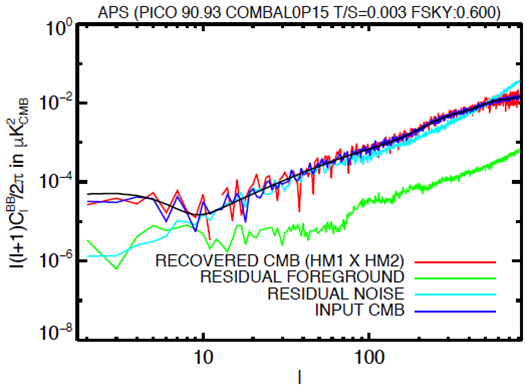
\includegraphics[width=3.0in]{images/soumen_NILC_foregrounds_93.png}}}
\hspace{0.25in}
\parbox{3.0in}{
\caption{The power spectrum of residual $BB$ foregrounds (green) has lower level than both the input CMB (blue) and the recovered CMB (red) which match well each other and the underlying cosmological model (black) after foreground separation with the NILC algorithm. This exercise assumed use of 60\% of the sky.   
\label{fig:nilc}}}
\vspace{-0.1in}
\end{figure}

Our results validate the need for a broad frequency coverage with a strong lever arm on Galactic emissions outside of the primary CMB bands. Figure~\ref{fig:psm_mr} shows that removing several of PICO's frequency bands, particularly those that monitor dust and synchrotron at high and low frequencies, respectively, significantly biases the extracted $BB$ power spectrum, particularly at the lowest $\ell$ values. 


There is other evidence that PICO could reach its stated target of $\sigma(r) = 0.0001$. Map-based simulations that were carried out for the forthcoming CMB-S4 experiment have shown that it can reach levels of $\sigma(r) = 0.0005$ in small, 3\%-size, clean patches of the sky. The analysis only used frequencies up to 300~GHz. In principle, even smaller patches of 1-2\% size are sufficient, and preferable, for attaining as low $\sigma(r)$ as possible. The PICO noise level per sky pixel is similar to that of CMB-S4, but PICO will have {\it full} sky coverage and thus access to {\it all} the clean patches available. Data from \planck\ indicate that there are $\sim10$ %\comor{check!} 
patches as clean, or cleaner than those used for the CMB-S4 analysis, indicating that PICO's $\sigma{r}$ could be $\sim3$ times more stringent. This scaling is very conservative because it only assumes CMB-S4's much narrower breadth of frequency coverage and its 7 bands; % \comor{check}; 
it neglects PICOs much stronger rejection of foregrounds with 21 bands and up to 800~GHz.  We note that if there {\it is} a detection of the \ac{IGW} signal with $r=0.001$, PICO will make it with high significance in multiple independent patches of the sky. 

Results from the Fisher-based analytic calculations give $\sigma(r) = 9 \cdot 10^{-5}$, and indicate a very small foreground residual with an $r_{eff} = 9 \cdot 10^{-7}.$

While our results are encouraging, as they suggest that PICO's frequency coverage and sensitivity will be adequate for this level of $r$, more work should be invested to gain complete confidence. This work includes running numerous realizations of different sky models, and analyzing them with various techniques; optimizing sky masks; and using combination of techniques to handle large, intermediate, and small angular scale foregrounds differently. 
\begin{figure}
%\hspace{-0.1in}
%\parbox{4.5in}
{\centerline {
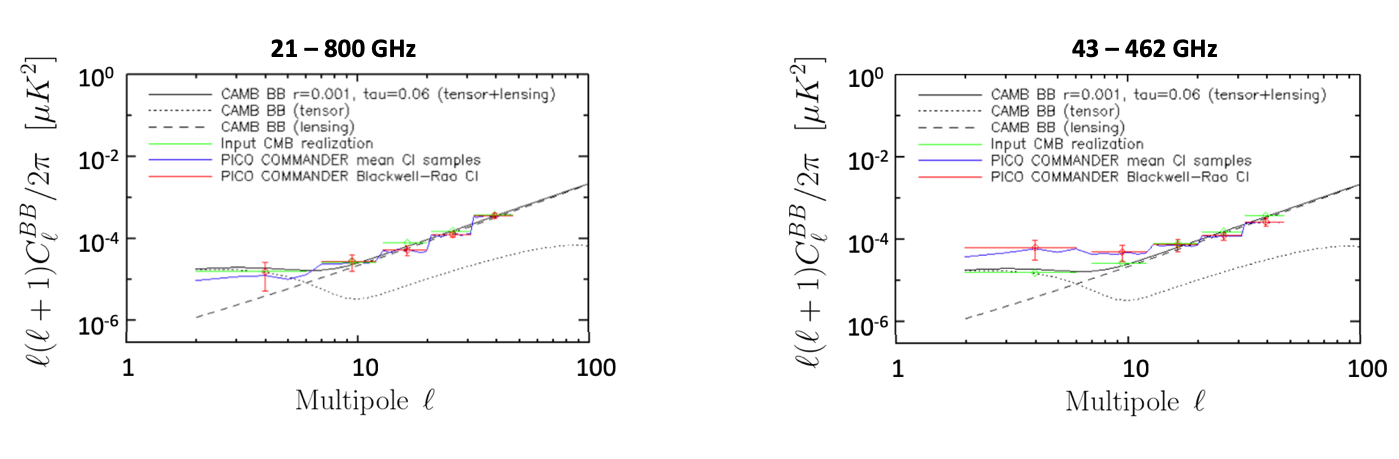
\includegraphics[width=4.5in]{images/commander_foregrounds_BB.png} }}
%\hspace{0.in}
%\parbox{2.0in}{
\caption{Foreground removal with all of PICO's 21 frequency bands (left panel) recovers the input CMB (green) without any bias (red) using the Commander algorithm on the \planck\ sky model (with 4~deg pixels, \comor{and 60\%} sky fraction). Running the same algorithm on the same sky without several of the lowest and highest bands (right panel) produces an output spectrum (red) that is biased relative to the input (green) at low $\ell$ multipoles. The bias would be interpreted as higher value of $r$ relative to the model input (solid black) with $r=0.001$ (dots) and lensing (dash). 
\label{fig:commander}}
\vspace{-0.0in}
\end{figure}


%\begin{figure}
%\hspace{-0.1in}
%\parbox{4.5in}{\centerline {
%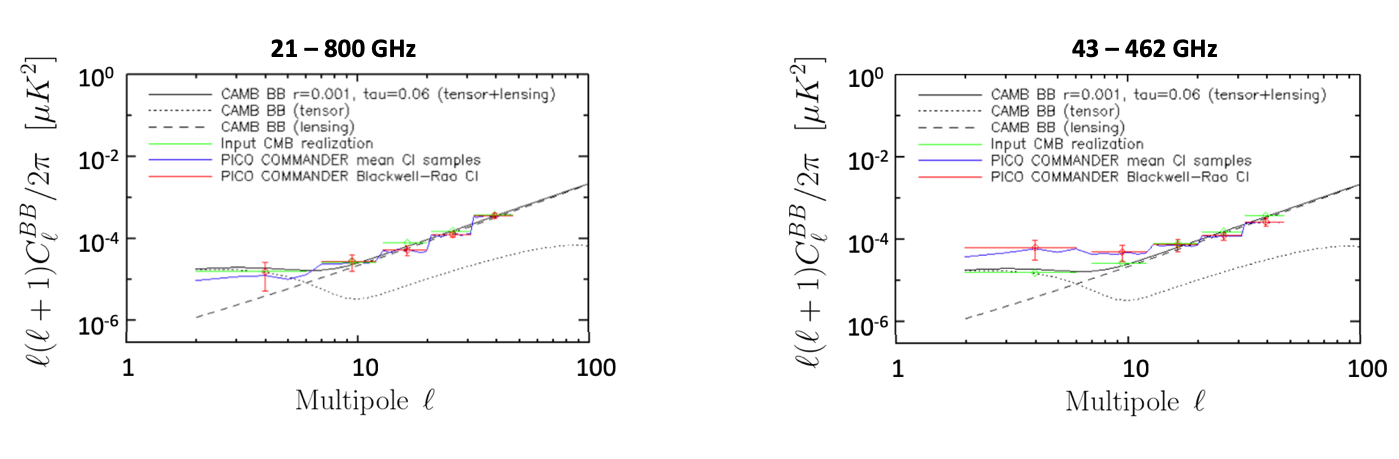
\includegraphics[width=4.5in]{images/commander_foregrounds_BB.png}}}
%\hspace{0.in}
%\parbox{2.0in}{
%\caption{Foreground removal with all of PICO's 21 frequency bands (left panel) recovers the input CMB (green) without any bias (red) using the Commander algorithm on the \planck\ sky model (with 4~deg pixels, \comor{and 60\%} sky fraction). Running the same algorithm on the same sky without the lowest and highest bands (right panel) produces an output spectrum (red) that is biased relative to the input (green) at low $\ell$ multipoles. The bias would be interpreted as higher value of $r$ relative to the model input (solid) with $r=0.001$ (dots) and lensing (dash). 
%\label{fig:commander}}}
%\vspace{-0.1in}
%\end{figure}


\end{document}

%\begin{figure}[!htb]
%\centering
%
\includegraphics[width=4cm]{images/example}
%\caption{example}
%\label{fig:im_3}
%\end{figure}

%The most important lesson arising from our exercise is that more work is required to ascertain that levels of $r \lesssim 0.001$ can be determined robustly on the largest angular scales, that is from the reionization peak.  Figure~\ref{fig:nilc} shows results from the NILC analysis. For several of the sky models the power spectra of the residual level of foregrounds -- that is the level of foregrounds remaining in the map after foreground separation -- is below the cosmological \ac{IGW} level with $r =0.003$. For a minority of the models, the residual is higher at $\ell \lesssim 20$. Results from GNILC, shown in Figure~\ref{fig:gnilc}, are similar. In all cases, the analyses are carried out using 60\% of the sky, the results shown are from one realization, and that no further optimization of the basic foreground separation technique has yet been applied. 

%More work is also required to understand the necessary span of frequencies required. Figure~\ref{fig:psm_mr} shows that removing several of PICO's frequency bands, in this case the three highest, significantly biases the extracted $BB$ power spectrum, particularly at the lowest $\ell$ values. This result should not be interpreted as conclusively demonstrating that a frequency span up to 800 GHz has been proven to be essential. At this point of time, different input sky models, coupled to different foreground separation techniques may yield different results. Rather, the conclusion is that further improvement in our modeling and analysis is required. 



%The baseline design of PICO has 21 channels observing the sky in the 20\,GHz to 800\,GHz frequency range (Fig.~\ref{fig:pico-channels-and-fg}). By analysing how the total emission varies across frequency bands, one can infer the detailed emission properties of the various emission components, form linear combinations of the observations that maximise the contribution of a component of interest while minimising contamination by the others and by instrumental noise, and understand the properties of the foregrounds to evaluate potential residuals in the CMB B-mode map. Various such techniques have been successfully used in previous CMB observations such as those of the Planck mission. Building on this existing expertise, we have carried out map based simulations within a ``data challenge'' framework to assess the capacity of PICO to measure the main signal of interest (CMB primordial B-modes). In this process one group prepares sets of simulated maps for different models of foreground emission of varying complexity from optimistic to pessimistic, which are placed in a shared area. These are then re-analyzed by multiple individuals and groups employing various different component separation algorithms.



\subsection{Systematic Errors}
\documentclass[PICOReport.tex]{subfiles}

%\newcolumntype{L}[1]{>{\raggedright\let\newline\\\arraybackslash\hspace{0pt}}m{#1}}
%\newcolumntype{K}[1]{>{\raggedright\centering\arraybackslash}m{#1}}

\begin{document}

Some of the PICO science goals attempt to detect extremely faint signals. The most ambitious one is to reach the  
signals characterizing an inflationary gravity wave with $r\lesssim0.001$, with a B-mode polarization peak signal $\lesssim10$nK in amplitude at $\ell=80$.
It has long been recognized that exquisite control of systematic uncertainties will be required for any experiment attempting 
to reach these levels, and it is widely accepted that the stability provided aboard a space platform makes it best suited to
control systematic uncertainties compared to other platforms. This is one of the most compelling reasons to observe the 
CMB from space.  As WMAP and \planck~ demonstrated, an L2 orbit offers excellent stability as well 
as the flexibility in the choice of scan strategy.  
PICO takes advantage of an L2 orbit, using a rotating spacecraft (at 1 rpm) whose spin axes precesses with a 10 hour period, thus scanning the sky in a way that is crosslinked on many time scales and at many angles, without interference from the Sun, Earth, or Moon, thus reducing the effects of low frequency excess noise without additional modulation. 
The redundancy of observations allows the checking of consistency of results and an improved ability to calibrate and to correct systematic errors in post-processing analysis.

A rich literature investigates the types of systematic errors due to the environment, the instrumentation, observation strategies, and data analysis that confound the polarization measurement by creating a bias or an increased variance\cite{hu03,shimon2008,yadav2010}. 
Every measurement to date has  reached a systematic error limit, and have advanced many sophisticated techniques to mitigate systematics, finding both new technological solutions and new analysis techniques.
As an example, the BICEP's systematics limited it to r=0.1\cite{Takahashi2010} while through additional effort within the program, BICEP2 achieved a systematics limit of r=6$\times$10$^{-3}$\cite{BICEP2_III}).
In the near term, the ground based and suborbital CMB community will continue to develop new techniques in handling systematics, particularly in developing the CMB-S4 project.

All prior on-orbit measurements of CMB polarization were limited by systematic errors until an in-depth study of the systematics was performed and the post-processing data analysis suppressed them\cite{Bennett13,planck2016_xlvi,Planck2018_I}. 
Particularly we note Fig. 3 of \cite{Planck2018_I} which quantifies Planck's systematic error limits on the polarization power spectral measurements.
Recently studied space missions, such as EPIC-IM, LiteBird and  \core, have placed
systematic error mitigation at the forefront of the case for their
mission and have developed tools and strategies for estimating and mitigating these\cite{hazumi2012,wallis2017,Natoli2018}.

Systematics are coupled with the
spacecraft scan strategy, and the details of the 
data analysis pipeline.
Thus, end-to-end simulation of the experiment is an essential tool,
including realistic instabilities and non-idealities of the spacecraft,
telescope, instrument and folding in data post-processing techniques
used to mitigate the effects.    

\subsubsection{List of Systematics}
The systematic errors faced by PICO can be categorized into three broad categories: 
1) Intensity-to-polarization leakage, 2) stability, and 3) straylight, and are listed in Table \ref{tbl:SystematicsList2col}. 
These were prioritized for further study using a risk factor incorporating the working group's assessment of how mission-limiting the effect is, how well these effects are understood by the community and whether mitigation techniques exist.  

The three highest risk systematic errors were studied further and are discussed in subsections below.  The PICO team used 
 simulation and analysis tools developed for Planck\cite{plank2015_xii_focalplane} and \core, adapting them for PICO.

%We note that many of the systematics could be mitigated further through the use of polarization modulation such as a half-wave plate or a variable phase delay modulator.  
%For the purposes of the cost constraints of PICO, we investigated mitigation techniques that do not require a modulator.  

\begin{table}[h!]
\hspace{-0.1in}
\parbox{3.4in}{
\centering
\scriptsize
 \begin{tabular}{p{3.3cm} p{0.5cm} p{1.4cm} p{1.7cm}}
 \hline
\textbf{Name} & \textbf{Risk}&\textbf{Effect} \\
 \hline
\textbf{Leakage}& &\\
Polarization Angle Calibration\dotfill& 
5&
$E{\to}B$ &
See Sect.~\ref{sec:angle}.
\\
 Bandpass Mismatch\dotfill&
 4& 
$T{\to}$P, $E{\to}B$  
   \\
Beam mismatch\dotfill& 
4&
$T{\to}$P, $E{\to}B$
& See Sect.~\ref{sec:angle}
\\
Time Response Accuracy and Stability\dotfill&
4&
$T{\to}$P, $E{\to}B$
\\
Readout Cross-talk\dotfill& 
4&
spurious P
\\
Chromatic beam shape\dotfill&
4&
spurious P
\\

Gain mismatch\dotfill&
3&
$T{\to}$P   
\\


Cross-polarization\dotfill&
3&
$E{\to}B$
\\
\hline 
\textbf{Stability} & & \\
Gain Stability\dotfill& 
5&
$T{\to}$P, $E{\to} B$
& 
See Sect.~\ref{sec:gain}
\\
Pointing jitter\dotfill&
3&
$T{\to}$P, $E{\to}B$
\\

\hline
\textbf{Straylight}& & \\
Far Sidelobes\dotfill& 
5&
spurious P
&
See Sect.~\ref{sec:fsl}.\\
 \hline
\textbf{Other} \\
Residual correlated noise (cosmic ray hits)\dotfill&
3 &
increased variance
\\
\hline
 \end{tabular}
}
\hspace{-0.0in}
\parbox{3.1in}{
\caption{\label{tbl:SystematicsList2col} Systematic errors expected in \pico's measurement of CMB polarization. Each source of systematic errors was given a rating of the risk that a given systematic error will dominate the B-mode measurement.  A risk level of 5 indicates that a systematic effect is highly significant because it is design-driving, has limited past experiments, and/or isn't well understood.  Risk level of 4 indicates a systematic that is either known to be large but is understood reasonably well or a smaller effect that requires precise modeling.  Risk level of 3 indicates that we expect the effect to be small, but it isn't necessarily well understood enough that modeling it should be done in detail in a mission Phase A. This study investigated the systematics with risk levels of 5 via simulations.}}
\hspace{-0.0in}
\end{table}

%\begin{table}[h!]
%\centering
%\scriptsize
% \begin{tabular}{p{3.3cm} p{0.5cm} p{1.5cm} p{4.5cm} p{2.8cm}}
% \hline
%\textbf{Name} & \textbf{Risk}&\textbf{Effect} & \textbf{State-of-the-art} & \textbf{Additional Mitigation Needed} \\
% \hline
%\textbf{Leakage}& &\\
%Polarization Angle Calibration\dotfill& 
%5&
%E$\to$B
%& 
%Knowledge of astrophysical calibrators to 0.3$^\circ$\citep{Aumont+2018}; ground measurement to 0.9$^\circ$ reconstruction to 0.2$^\circ$ using $TB$ and $EB$ demonstrated by \planck\citet{Planck_Lowell}
%& 
%See Sect.~\ref{sec:angle}.
%\\
% Bandpass Mismatch\dotfill&
% 4& 
%T$\to$P, E$\to$B  & Precise bandpass measurement\cite{Pajot_2010};
%SRoll algorithm\cite{Planck_Lowell}; filtering technique\cite{CORE_systematics}. &
%SOA meets req't
%   \\
%Beam mismatch\dotfill& 
%4&
%T$\to$P, E$\to$B
%& See Sect.~\ref{sec:angle} & none\\
%Time Response Accuracy and Stability\dotfill&
%4&
%T$\to$P, E$\to$B&
%On-orbit reconstruction to 0.1\% across a wide signal band\cite{planck2013_vii}, residuals corrected as part of beam and map-making algorithm\cite{Planck_Lowell}.
%& SOA meets req't
%\\
%Readout Cross-talk\dotfill& 
%4&
%spurious P
%&
%\planck\ high-impedence bolometers: 10$^{-3}$ crosstalk did not impact CMB polarization\cite{Planck_Lowell}.  Cross-talk of low-impedence bolometers is 0.3\%\cite{BICEP2_II}.
%&
%SOA meets req't
%\\
%Chromatic beam shape\dotfill&
%4&
%spurious P
%&
%\planck\ simulations and parameterization as part of the likelihood.
%&
%%Should be further investigated in Phase A of a mission using physical optics simulations.
%Mission-specific simulations needed.  
%\\
%
%Gain mismatch\dotfill&
%3&
%T$\to$P &
%mission-average relative calibration demonstrated to 10$^{-4}$ to 10$^{-5}$ level \cite{Planck_Lowell}
%&
%SOA meets req't  
%\\
%
%
%Cross-polarization\dotfill&
%3&
%E$\to$B
%&
%Degenerate with polarization gain calibration.
%&
%SOA meets req't
%\\
%\hline 
%\textbf{Stability} & & \\
%Gain Stability\dotfill& 
%5&
%T$\to$P, E$\to$B
%& 
%Reconstruction of time variability of gain to 0.2\% in \planck\cite{Planck_Lowell}.
%&
%See Sect.~\ref{sec:gain}
%\\
%Pointing jitter\dotfill&
%3&
%T$\to$P, E$\to$B
%&
%Pointing reconstruction in \planck\ to 0.8 and 1.9 arcsec in-scan and cross-scan \cite{planck2016_l}
%&
%SOA meets req't
%\\
%
%\hline
%\textbf{Straylight}& & \\
%Far Sidelobes\dotfill& 
%5&
%spurious P
%& 
%\planck\ validated straylight model in anechoic chamber to -80~dBi\cite{Tauber2010}.
%&
%See Sect.~\ref{sec:fsl}.\\
% \hline
%\textbf{Other} \\
%Residual correlated cosmic ray hits\dotfill&
%3 &
%increased variance
%&
%\planck/HFI's 5\% percent noise correlation did not impact results\cite{Planck_Lowell}. 
%&
%SOA detector design to reduce cosmic ray cross-section; SOA analysis techniques meet req't
%\\
%\hline
% \end{tabular}
%\caption{\label{tbl:SystematicsList} Systematic errors expected in \pico's measurement of CMB polarization.}
% \end{table}

\subsubsection{Absolute polarization angle calibration}
\label{sec:angle}

CMB polarization can be rotated due to 1. a birefringent primordial Universe, or a Faraday rotation
due a primordial magnetic field \citep{Pogosian+2018}, 2. birefringent
foregrounds, or interaction with the Galactic magnetic field,
3. systematic effects in the instrument, and in particular an error on
the direction of polarization measured by each detector.  
While the first two sources create a rotation that may depend on scale,
position and/or frequency, the latter depends mainly on
the detector. 

A rotation {\prang} of the direction of polarization mixes the $Q$ and $U$ Stokes parameters via
$Q\pm iU \longrightarrow e^{\mp i 2 \prang} (Q\pm iU)$
and thus mixes the the power spectra and their correlations as illustrated in Fig.~\ref{fig:rot_bb_tb_eb}.
% via (assuming the rotation to be independent on scale and location)
%\begin{subequations}
%\begin{align}
%C^{TT}_\ell &\longrightarrow & C^{TT}_\ell                                             &= & C^{TT}_\ell \\
%C^{TE}_\ell &\longrightarrow & \cos 2\prang\  C^{TE}_\ell                                &\sim & \left(1 - 2\prang^2\right)\ C^{TE}_\ell \\
%C^{EE}_\ell &\longrightarrow & \cos^2 2\prang\  C^{EE}_\ell + \sin^2 2\prang\  C^{BB}_\ell &\sim & C^{EE}_\ell - 4\prang^2\ \left(C^{EE}_\ell - C^{BB}_\ell\right) \\
%C^{BB}_\ell &\longrightarrow & \sin^2 2\prang\  C^{EE}_\ell + \cos^2 2\prang\  C^{BB}_\ell &\sim & C^{BB}_\ell + 4\prang^2\ \left(C^{EE}_\ell - C^{BB}_\ell\right)\\
%C^{TB}_\ell &\longrightarrow & \sin 2\prang\  C^{TE}_\ell                                &\sim & 2\prang\  C^{TE}_\ell \\
%C^{EB}_\ell &\longrightarrow & \sin 2\prang \cos 2\prang \left(C^{EE}_\ell -  C^{BB}_\ell\right)  &\sim & 2\prang\ \left(C^{EE}_\ell -  C^{BB}_\ell\right)
%\end{align}
%\end{subequations}


%------------------------------------------------------------------------------------------
\begin{figure}[htb]
\includegraphics[width=0.6\textwidth]{images/PICO_rotate_eb4_v2.\suffix} 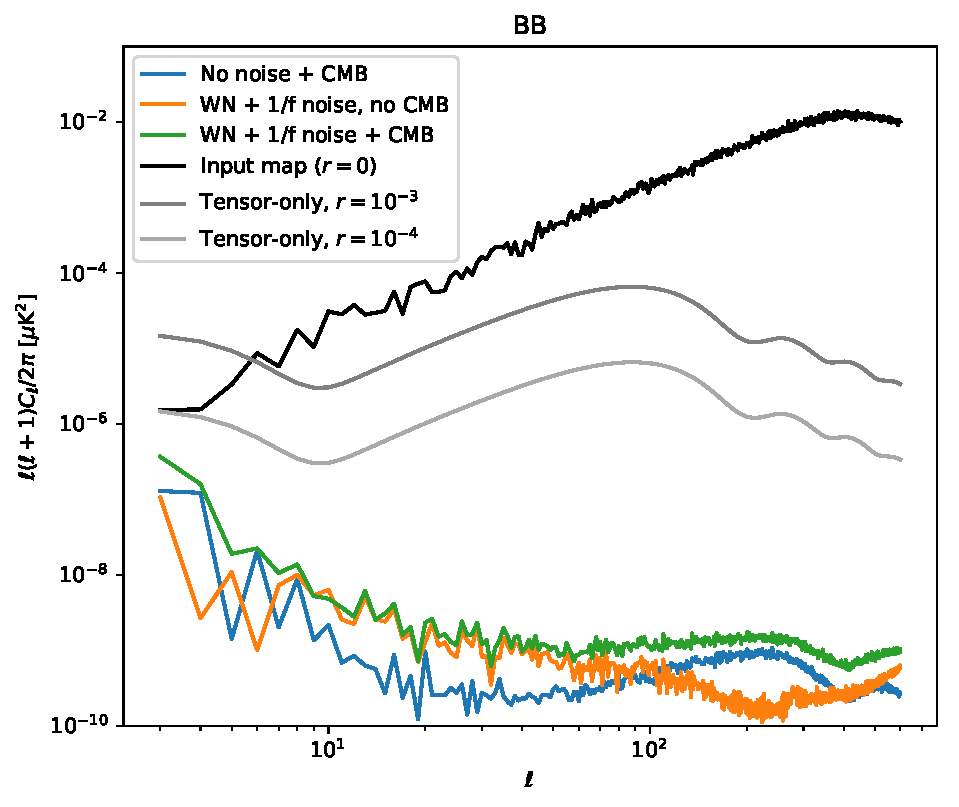
\includegraphics[width=0.4\textwidth]{images/calibration_spectrum_BB.pdf}
\caption{\label{fig:rot_bb_tb_eb} Left and center: Spurious power due to a rotation of the angle of polarization, assuming the Planck 2018 $\Lambda$-CDM model \citep{Planck2018_VI} with $\tau=0.054$ and expected \pico\ noise performance, assuming removal of 85\% of the lensing power.  Right: residual power after removal of temporal gain drifts using the dipole.}
\end{figure}
%------------------------------------------------------------------------------------------
%
%------------------------------------------------------------------------------------------
%\begin{figure}[htb]
%\includegraphics[width=0.40\textwidth]{images/PICO_sens2_v0_F5p0_f0p5_n0p62_k4_a1p0_2_4000.\suffix}
%\includegraphics[width=0.40\textwidth]{images/PICO_sens2_v0_F15p0_f0p5_n0p62_k4_a1p0_2_4000.\suffix}
%\caption{\label{fig:rot_sens_0} Upper panels: signal to noise ratio of the polarization angle {\prang} measurement
%by $EB$ (blue lines), $TB$ (green lines) and $BB$ (red lines), assuming either no delensing (solid lines) 
%or perfect delensing (dashes); the shaded area is $|\prang|/\sigma_\prang < 3$.
%Lower panels: degradation on measurement of $r$, for $r=10^{-2},\ 10^{-3},\ 10^{-4}$ (magenta, orange and cyan lines, respectively),
%either with no delensing (solid lines) or perfect delensing (dashes).
%The underlying cosmology is Planck 2018 $\Lambda$-CDM model (with $\tau = 0.054$), and assuming a polarized noise of rms = $0.62 \mu K.\arcmin$ and power spectrum $(1 + (\ell_{\rm knee}/\ell)^n)$ with $\ell_{\rm knee}=4$ and $n=1$, with the analysis done on the multipole range $[2,4000]$ over a sky fraction $\fsky=0.5$. The beam FWHM$=5\arcmin$ on the \emph{lhs} and $15\arcmin$
%on the \emph{rhs} panels. \EFH{Probably remove this figure and summarize in text.}}
%\end{figure}
%
% \begin{figure*}[htb]
% \includegraphics[width=0.5\textwidth]{fig_efh/PICO_sens2_v0_F15.0_f0.5_n0.62_k4_a1.0_2_4000.\suffix}
% \caption{\label{fig:rot_sens_1} Same as Fig.~\ref{fig:rot_sens_0}, with a FWHM=$15\arcmin$.}
% \end{figure*}
%
%\begin{figure}[htb]
%\includegraphics[width=0.40\textwidth]{images/PICO_sens2_v0_F5p0_f0p5_n0p62_k4_a1p0_20_4000.\suffix}
%\includegraphics[width=0.40\textwidth]{images/PICO_sens2_v0_F5p0_f0p5_n1p86_k4_a1p0_2_4000.\suffix}
%\caption{\label{fig:rot_sens_2} Same as Fig.~\ref{fig:rot_sens_0}, left panels, reducing the multipole range $[20,4000]$ (\emph{lhs}) or with a noise rms multiplied by 3 (\emph{rhs}).\EFH{Probably remove this figure and summarize in text.}}
%\end{figure}
% %
% \begin{figure*}[htb]
% \caption{\label{fig:rot_sens_3} Same as Fig.~\ref{fig:rot_sens_0}, with a noise rms multiplied by 3.}
% \end{figure*}
% %------------------------------------------------------------------------------------------

The most recent constraints on cosmological birefringence \citep{Planck2016_XLIX} were limited by uncertainties on the detector orientations.  In Planck, the detectors were characterized pre-launch to $\pm 0.9\degree$ (rel.) $\pm 0.3\degree$ (abs.) \citep{Rosset+2010}. For \pico, the relative rotation of the detectors will be measured to a few $0.1\arcmin$ using the CMB, but the overall rotation is unlikely to be known pre-launch to better than Planck.  Known polarized sources, such as the Crab Nebula, are not characterized well enough independently to serve as calibrators; \citet{Aumont+2018} show that the current uncertainty of $0.33\degree = 20\arcmin$ on the Crab polarization orientation, limits a $B$ mode measurement to $r \sim 0.01$, far from \pico's target.

%Figures \ref{fig:rot_sens_0} and \ref{fig:rot_sens_2} show how the measurement of $r$ by \pico\ is degraded because of an overall rotation of polarization, and how $TB$ and $EB$ can be used to monitor this rotation, assuming that the only source of polarization rotation is instrumental.
%These results are obtained assuming the spectra to have a Gaussian likelihood, with a variance $\propto 1/\fsky$, and ignoring the foreground contributions.

In the absence of other systematics and foregrounds, a polarization rotation error $\alpha$ of $10\arcmin$ degrades 
the error bar of $r$ by 30\%, while $EB$, $TB$ and $BB$ spectra can measure a rotation $\alpha$ at 3$\sigma$ when $\alpha \sim 0.07, 0.2$  and $0.9\arcmin$ respectively
 on perfectly delensed maps, and $0.25, 0.9$ and $4.5\arcmin$ on raw maps.

In principle, the technique of using the $TB$ and $EB$ spectra can detect and measure a global polarization rotation error at levels ($~0.1 \arcmin$) below those affecting $r$ measurements in $BB$ ($> 1 \arcmin$).  However, a future mission should simulate additional aspects, such as delensing, the interaction with foregrounds, and $1/f$ noise in simulating and assessing the impact of an angle calibration error.

\subsubsection{Gain Stability}
\label{sec:gain}

%------------------------------------------------------------------------------------------

%\begin{figure}[htb]
%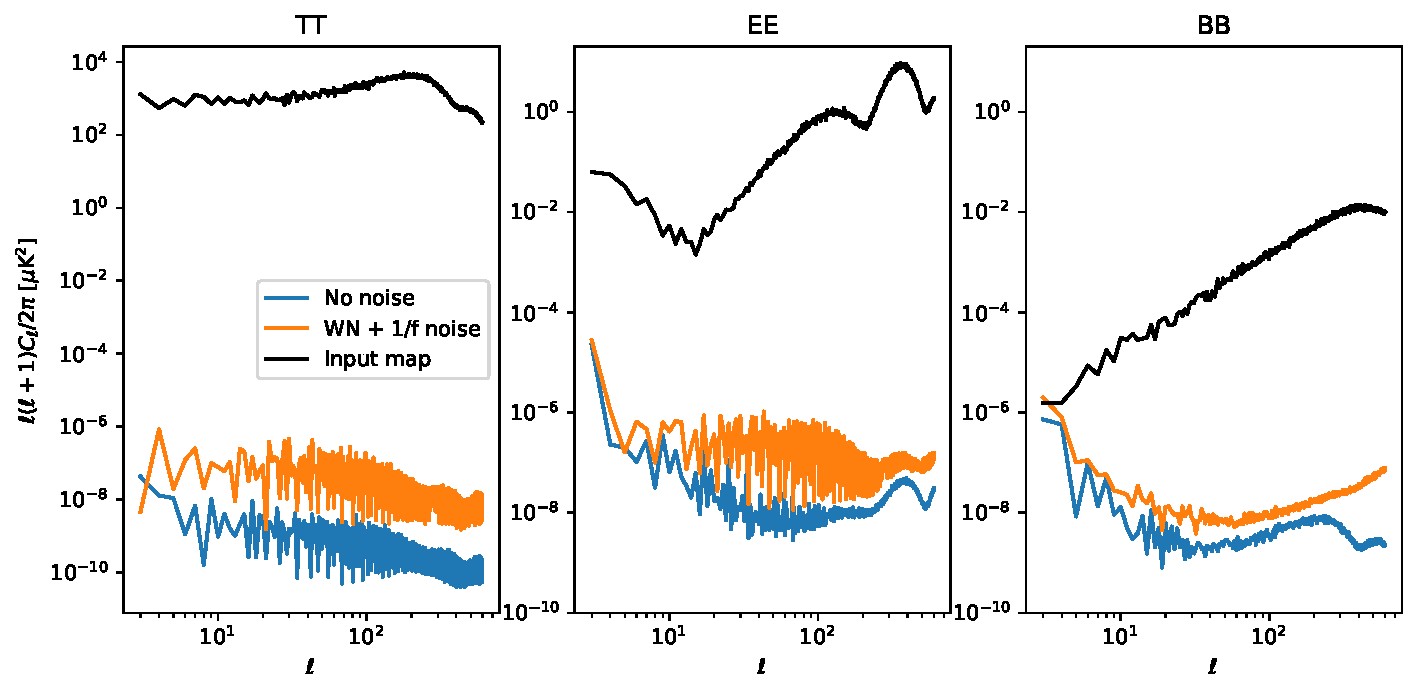
\includegraphics[width=0.7\textwidth]{images/calibration_spectra.pdf}
%\caption{\label{fig:calibration_spectra} Residual power due to calibration.}
%\end{figure}
%------------------------------------------------------------------------------------------

Photometric calibration is the process of converting the raw output of the receivers into astrophysical units via the characterization of the \emph{gain factor} $G(t)$ which we allow to vary with time.  In space, $G(t)$ can be measured with the dipole.   For the PICO concept study, we evaluated the impact of noise in the estimation of $G(t)$ using the tools developed for the Planck/LFI instrument and the CORE mission proposal. The quality of the estimate depends on the noise level of the receivers, but also on the details of the scanning strategy. 
To analyze the impact of calibration uncertainties on PICO, we performed  the following analysis:1. We simulated the observation of the sky, assuming four receivers, the nominal scanning strategy, and $1/f$ noise. The simulated sky contained CMB anisotropies, plus the CMB dipole. 2. We ran the calibration code to fit the dipole against the raw data simulated during step~1. 3. We again simulated the observation of the sky, this time using the values of $G$ computed during step~2, which contain errors due to the presence of noise and the CMB signal.

The presence of large-scale Galactic emission features can bias the estimation of calibration factors. Ideally, a full data analysis pipeline would pair the calibration step with the component separation step, following a schema similar to Planck/LFI's legacy data processing\cite{Planck2018_II}: the calibration code is followed by a component separation analysis, and these two steps are iterated until the solution converges.

Results of the simulation (neglecting foregrounds) are shown as power spectrum residuals in Fig.~\ref{fig:rot_bb_tb_eb}. 
We estimate the gain fluctuations to better than 10$^{-4}$ solving for the gain every 40 hours (4 precession periods).
The scanning strategy employed by PICO allows for a much better calibration than Planck, thanks to the much faster precession.

\subsubsection{Far Sidelobe Pickup}
\label{sec:fsl}
%The main beam (within a few degrees of the axis of beam response) in a CMB mission can be measured to high precision using the planets .  
Measurement of each detector's response to signals off axis, which tends to be weak (--80dB less than the peak response) but spread over a very large solid angle, is difficult to do pre-launch, and may not even be done accurately after launch.  Nonetheless, this far sidelobe can couple bright Galactic signal from many tens of degrees off-axis and confuse it with polarized signal from the CMB off the Galactic plane.    To evaluate this systematic error, GRASP software\footnote{https://www.ticra.com} was used to compute the \pico\ telescope's response over the full sky.  The computed full-sky beams showed features peaking at about -80\,dB of the on-axis beam.   This full-sky beam was convolved with a polarized Galactic signal and a one-year \pico\ mission scan using the simulation pipeline and preliminarily shows that the far sidelobe pickup must be calculated accurately down to the 90 dB level in order to be removed from the measured B-mode signal to a level that does not appreciably increase the variance on the B-mode power measurement.


\subsubsection{Key Findings}
Properly modeling, engineering for, and controlling the effects of systematic errors in a
next-generation CMB probe is critical.  As of today, we conclude that there is a clear path to demonstrate that state-of-the-art technology and data processing can take advantage of the L2 environment and control systematic errors to a level that enables the science goals of PICO. In particular we note:
\begin{itemize}
\item The raw sensitivity of the instrument should include enough margin
that data subsets can independently achieve the science goals.
This allows testing of the results in the data analysis and additional
data cuts, if needed.
\item In a PICO mission, a physical optics model of the telescope should be developed, enabling full-sky beam calculations, which should be validated as much as possible on the ground.  This will be needed to characterize and remove far sidelobe pickup seen during the mission. 
\item NASA's support of ground-based and suborbital CMB missions will mitigate risk to a future space mission as PICO by continuing to develop analysis techniques and technology for mitigation of systematic errors.

\item In a PICO mission's phase A, a complete end-to-end system-level
simulation software facility would be developed to assist the team in setting 
requirements and conducting trades between subsystem requirements while
realistically accounting for post-processing mitigation.  Any future
CMB mission is likely to have similar orbit  
and scan characteristics to those of PICO, thus there is an opportunity for NASA and
the CMB community to invest in further development of this capability now.
\end{itemize}

\end{document}

%\begin{figure}[!htb]
%\centering
%
\includegraphics[width=4cm]{images/example}
%\caption{example}
%\label{fig:im_3}
%\end{figure}


\section{Instrument Implementation (10 pgs)}
\documentclass[../PICOReport.tex]{subfiles}

\begin{document}
blah

\begin{figure}[!htb]
\centering

\includegraphics[width=4cm]{../images/example}
 
\label{fig:im_example}
\caption{example}
\end{figure}


\end{document}

\section{Mission Implementation (5 pgs)}
\documentclass[PICOReport.tex]{subfiles}

\begin{document}

To be included: mission architecture, spacecraft and subsystems, orbit, attitude control and determination (Trangsrud)


\end{document}

%\begin{figure}[!htb]
%\centering
%
\includegraphics[width=4cm]{images/example}
%\caption{example}
%\label{fig:im_3}
%\end{figure}


\section{Technology Development (4 pgs)}
\documentclass[../PICOReport.tex]{subfiles}

\begin{document}
blah

\begin{figure}[!htb]
\centering

\includegraphics[width=4cm]{../images/example}
 
\label{fig:im_example}
\caption{example}
\end{figure}


\end{document}

\section{Cost (6 pgs)}
\documentclass[../PICOReport.tex]{subfiles}

\begin{document}
blah

\begin{figure}[!htb]
\centering

\includegraphics[width=4cm]{../images/example}
 
\label{fig:im_example}
\caption{example}
\end{figure}


\end{document}

\newpage

\bibliography{mybib}


\begin{acronym}
    %A
    \acro{ACS}{attitude control system}
    \acro{ADC}{analog-to-digital converters}
    \acro{ADS}{attitude determination software}
    \acro{AHWP}{achromatic half-wave plate}
    \acro{AMC}{Advanced Motion Controls}
    \acro{ARC}{anti-reflection coatings}
    \acro{ATA}{advanced technology attachment}
    %B
    \acro{BAO}{barion acoustic oscillations}
    \acro{BRC}{bolometer readout crates}
    \acro{BLAST}{Balloon-borne Large-Aperture Submillimeter Telescope}
    %C
    \acro{CANbus}{controller area network bus}
    \acro{CIB}{cosmic infrared background}
    \acro{CMB}{cosmic microwave background}
    \acro{CMM}{coordinate measurement machine}
    \acro{CSBF}{Columbia Scientific Balloon Facility}
    \acro{CCD}{charge coupled device}
    %D
    \acro{DAC}{digital-to-analog converters}
    \acro{DASI}{Degree~Angular~Scale~Interferometer}
    \acro{dGPS}{differential global positioning system}
    \acro{DfMUX}{digital~frequency~domain~multiplexer}
    \acro{DLFOV}{diffraction limited field of view}
    \acro{DSP}{digital signal processing}
    %E
    \acro{EBEX}{E~and~B~Experiment}
    \acro{EBEX2013}{EBEX2013}
    \acro{ELIS}{EBEX low inductance striplines}
    \acro{ETC}{EBEX test cryostat}
    %F
    \acro{FDM}{frequency domain multiplexing}
    \acro{FPGA}{field programmable gate array}
    \acro{FCP}{flight control program}
    \acro{FOV}{field of view}
    \acro{FWHM}{full width half maximum}
    %G
    \acro{GPS}{global positioning system}
    %H
    \acro{HDPE}{high density polyethylene}
    \acro{HIM}{high index materials}
    \acro{HWP}{half-wave plate} 
    %I
    \acro{IA}{integrated attitude}
    \acro{IGW}{inflationary gravity wave} 
    \acro{ILC}{independent linear combination}
    \acro{IP}{instrumental polarization} 
    %J
    \acro{JSON}{JavaScript Object Notation}
    %L
    \acro{LDB}{long duration balloon}
    \acro{LED}{light emitting diode}
    \acro{LCS}{liquid cooling system}
    \acro{LC}{inductor and capacitor}
    \acro{LZH}{Lazer Zentrum Hannover}
%M
    \acro{MCP}{multi-color pixel}
    \acro{MSM}{millimeter and sub-millimeter}    
    \acro{MLR}{multilayer reflective}
    \acro{MAXIMA}{Millimeter~Anisotropy~eXperiment~IMaging~Array}
    %N
    \acro{NASA}{National Aeronautics and Space Administration}
    \acro{NDF}{neutral density filter}
    %P
    \acro{PCB}{printed circuit board}
    \acro{PE}{polyethylene}
%    \acro{PTFE}{polytetrafluoroethylene}
    \acro{PME}{polarization modulation efficiency}
    \acro{PSF}{point spread function}
    \acro{PV}{pressure vessel}
    \acro{PWM}{pulse width modulation}
    %R
    \acro{RMS}{root mean square}
%S
    \acro{SLR}{single layer reflective}
    \acro{SMB}{superconducting magnetic bearing}
    \acro{SNR}{Signal to noise ratio}
    \acro{SQUID}{superconducting quantum interference device}
    \acro{SQL}{structured query language}
    \acro{STARS}{star tracking attitude reconstruction software}
    \acro{SWS}{sub-wavelength structures}
%T
    \acro{TES}{transition edge sensor}
    \acro{TDRSS}{tracking and data relay satellites}
   \acro{TM}{transformation matrix}
% U
    \acro{UHMWPE}{ultra high molecular weight polyethylene}   
    \acro{UMN}{University of Minnesota}
    
\end{acronym}


\end{document}


